\documentclass{article}
\usepackage{graphicx} % Required for inserting images
\usepackage{authblk} % Required for author affiliations
\usepackage{indentfirst} % Indent first paragraph of sections
\usepackage{amssymb} % For mathematical symbols
\usepackage{amsthm} % For theorem environments
\usepackage{amsmath} % For advanced math typesetting
\usepackage{hyperref}
\usepackage{enumitem}
\usepackage{pgfplots} % For plots
\usepackage{tikz} % For drawing shapes
\usepackage{circuitikz}
\usepackage{float} % For [H] float option
\usepackage{booktabs} % Better rules for tables (provides \toprule, \midrule, \bottomrule)
\usepackage{subcaption}

\pgfplotsset{compat=1.18} % Set compatibility level
\newtheorem{theorem}{Theorem}
\newtheorem{law}{Law}
\newtheorem{principle}{Principle}
\newtheorem{definition}{Definition}
\newtheorem{problem}{Problem}
\newtheorem{solution}{Solution}
\newtheorem*{example}{Example}
\newtheorem{remark}{Remark}
\newtheorem{proposition}{Proposition}
\newtheorem{algorithm}{Algorithm}
\reversemarginpar
\hypersetup{
    colorlinks=true,
}
\begin{document}

% ===========================================================
%  Title page
% ===========================================================
\title{CHEM 396: Simulation of Amorphous Silicon using MLIPs}
\author{W.R.YCH.}
%prof Yelena (Lena) Simine
\date{August \(3^{rd}\), 2026}
\setcounter{Maxaffil}{0}
\renewcommand\Affilfont{\itshape\small}
\maketitle

% ===========================================================
%  Abstract
% ===========================================================
\noindent\rule{\textwidth}{0.4pt}
\thispagestyle{empty}
\begin{abstract}
    Models of amorphous silicon are generated by melt-quench molecular dynamics driven by Moment Tensor Potentials (MTPs) in LAMMPS on the Narval cluster. A custom LAMMPS build carrying the MTP pair styles was compiled and validated in both CPU and Kokkos GPU forms, the latter running a Lennard-Jones reference case roughly $16\times$ faster on an A100. Five silicon MTPs were then benchmarked: two melt-stable potentials at descriptor levels 22 and 26, and three pruned variants of increasing cost. A 216-atom diamond lattice was heated to 2500~K, held there for 1~ns, and cooled to 300~K at 1~K/ps, all under NPT at zero pressure.

    All five potentials completed a nanosecond in the liquid without instability, contrary to the expectation that the pruned variants would fail in a melt, and all five reproduce the reference liquid structure closely: mean coordination numbers agree to $1.0\%$ and tetrahedral order parameters to $3.1\%$, with no systematic trend against pruning level. The cost ordering follows the descriptor level cleanly, \texttt{pruned\_1} running $11.7\times$ faster than level 22 at fixed system size. That structural agreement does not survive the quench, where the amorphous densities split by $1.9\%$ in the direction predicted by an earlier fixed-volume pressure test. Structural characterisation of the quenched configurations is in progress and is the outstanding item of the project.
\end{abstract}
\noindent\rule{\textwidth}{0.4pt}
\clearpage

% ===========================================================
%  Table of Contents
% ===========================================================
\thispagestyle{empty}
\pagenumbering{gobble} 
{
  \hypersetup{linkcolor=black}
  \tableofcontents
}
\clearpage

% ===========================================================
\pagenumbering{arabic}
\setcounter{page}{1}

% ===========================================================
%  1. INTRODUCTION
% ===========================================================
\section{Introduction}
% Logistics: intermediate report July 27th (30%), oral presentation TBD (20%),
% final report TBD (50%). Project runs June 15th to Aug 31st, 2026.

Amorphous silicon (a-Si) lacks the long-range order of a crystal which its crystalline counterpart possesses. Most atoms are still bonded to four neighbours in roughly tetrahedral arrangements, but the bond lengths and angles vary rather than being fixed, a structure described by the continuous random network model. a-Si is used in solar cells, thin-film transistors, and battery anodes, and its properties depend strongly on coordination defects, where atoms have too few or too many bonds.

Simulating a-Si requires a model of the forces between atoms, which involves a tradeoff. Density functional theory (DFT) is accurate but computationally expensive, while empirical potentials\footnote{Empirical potentials are mathematical models that describe the interaction between atoms based on experimental data.} are fast but less flexible. Machine-learning potentials offer a middle ground by learning the energy from DFT data. This project uses one such method, the Moment Tensor Potential (MTP)~\cite{shapeev2016}.

The aim of this project is to generate models of a-Si through melt-quench molecular dynamics\footnote{You heat simulated silicon until it's liquid, then cool it fast so it freezes into a disordered solid.} simulations driven by an MTP, and to analyze the resulting structures using the Morphological Autoregressive Protocol (MAP).

% ===========================================================
%  2. BACKGROUND
% ===========================================================
\section{Background}

\subsection{Amorphous Silicon}

\subsubsection{Silicon}
\begin{definition}[Silicon]
    Silicon is a chemical element with atomic number 14, symbol Si. It is a metalloid with properties between metals and nonmetals, and is the second most abundant element in the Earth's crust after oxygen.
\end{definition}
\begin{definition}[Crystalline Silicon]
    Crystalline silicon (c-Si) is a solid form of silicon where atoms are arranged in a regular, repeating lattice structure, specifically the diamond cubic structure.
\end{definition}
Each silicon atom in the crystalline arrangement is $sp^3$ hybridized and covalently bonded to four neighbours in a tetrahedral geometry, with fixed bond lengths of ~2.35 Angstrom and angles of $109.5^\circ$.

The bulk modulus\footnote{The material's resistance to uniform compression or how much its volume decreases when subjected to hydrostatic pressure.} of c-Si is approximately $98 \text{ GPa}$ at room temperature and atmospheric pressure. This structure gives c-Si its characteristic properties, such as high thermal conductivity and semiconducting behaviour.

The density of c-Si is about $2.33 \text{ g/cm}^3$ at room temperature.

\begin{definition}[Amorphous Silicon]
    Amorphous silicon (a-Si) is a form of silicon that lacks long-range crystalline order, exhibiting a disordered atomic structure.
\end{definition}
The silicon atoms in the amorphous form are predominantly $sp^3$ hybridized, with the large majority of atoms remaining fourfold-coordinated and the rest forming coordination defects (\ref{C.D}).

Bond lengths stay close to the crystalline value at about 2.35 Angstrom, and bond angles centre on $109.5^\circ$ but broaden with a root-mean-square spread of roughly $10^\circ$.

The bulk modulus of a-Si is lower than that of c-Si, clustering around 70 to 80 GPa at room temperature and atmospheric pressure.

The density of a-Si is about $2.28 \text{ g/cm}^3$, a little less than that of c-Si.

\begin{figure}[H]
    \centering
    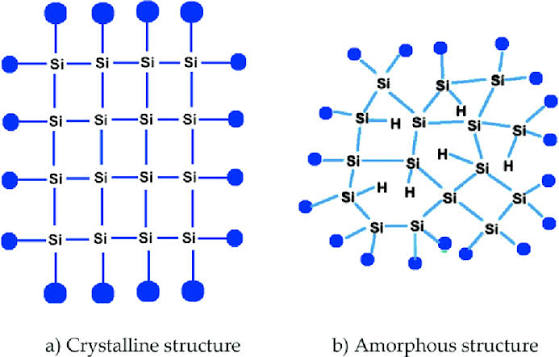
\includegraphics[width=0.8\textwidth]{c-Si-vs-a-Si.jpg}
    \caption{Schematic comparison of c-Si and a-Si.}
    \label{fig:crystalline_vs_amorphous}
\end{figure}

\subsubsection{The Continuous Random Network Model}

\begin{definition}[Continuous Random Network]
    The continuous random network (CRN) model describes amorphous materials as a network of atoms with no repeating long-range structure, while still preserving the preferred local bonding arrangement of each atom (i.e., silicon atoms are typically 4-fold\footnote{bonded to four neighbors} coordinated).
\end{definition}

Originally proposed for silica glasses ($SiO_2$), the model posits a non-crystalline, 3D network in which every silicon atom is perfectly fourfold-coordinated via covalent bonds.

The disorder enters not through coordination defects but through geometry: because the network is non-periodic, bond lengths and bond angles vary around their crystalline values rather than taking the fixed values set by a lattice. Fig.~\ref{fig:CRN} sketches this picture for a tetrahedral network.

\begin{figure}[H]
    \centering
    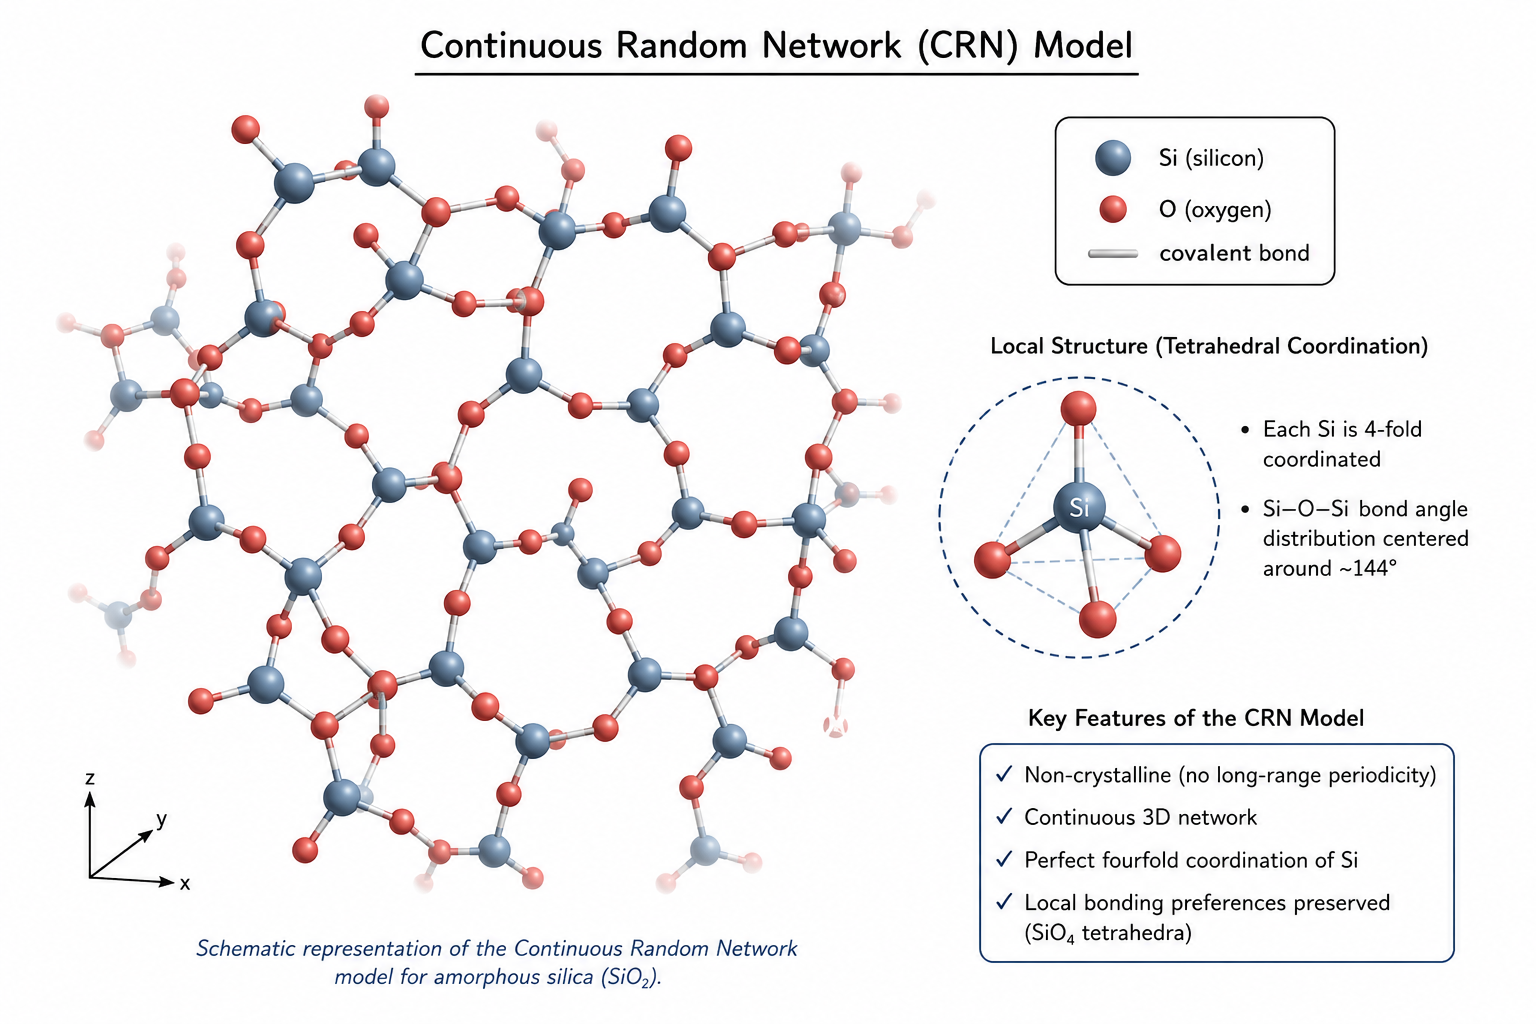
\includegraphics[width=1\textwidth]{Continuous Random Network.png}
    \caption{The continuous random network model of amorphous silica.}
    \label{fig:CRN}
\end{figure}

The geometric freedom in such a network is limited. For an amorphous solid to form a stable, fully connected network in the first place, its local bonding must satisfy a small set of structural constraints, first set out by Zachariasen~\cite{zachariasen1932}.

\begin{theorem}[Zachariasen's Rules for Glass Formation]
    \leavevmode
    \begin{itemize}
        \item No oxygen atom may be linked to more than two cations.
        \item The cation coordination number is small\footnote{For example, 3 for Boron and 4 for Silicon}.
        \item Oxygen polyhedra\footnote{A three-dimensional solid with flat faces and straight edges.} must share corners, not edges or faces.
        \item For 3D networks, at least three corners must be shared by polyhedra.
    \end{itemize}
\end{theorem}

Zachariasen's rules describe what a valid glass network must look like, but they tell us which structures are admissible without prescribing how to build one. To actually generate an atomic model that satisfies these constraints, we need an explicit procedure, which is precisely what the Wooten-Winer-Weaire algorithm provides~\cite{www1985}.

\begin{theorem}[Wooten-Winer-Weaire Algorithm]
    The Wooten-Winer-Weaire (WWW) algorithm is a foundational Monte Carlo method used to generate realistic, CRN models of amorphous tetrahedral semiconductors.
\end{theorem}

At the core of the algorithm is a local operation called a bond transposition. In this step, two nearby bonds are broken and the atoms are reconnected in a different way. This changes the local structure of the network while keeping each atom bonded to four neighbors. The new structure is then accepted or rejected using a Monte Carlo method based on how the strain energy changes. Fig.~\ref{fig:WWW_algorithm} illustrates this process.

\begin{figure}[H]
    \centering
    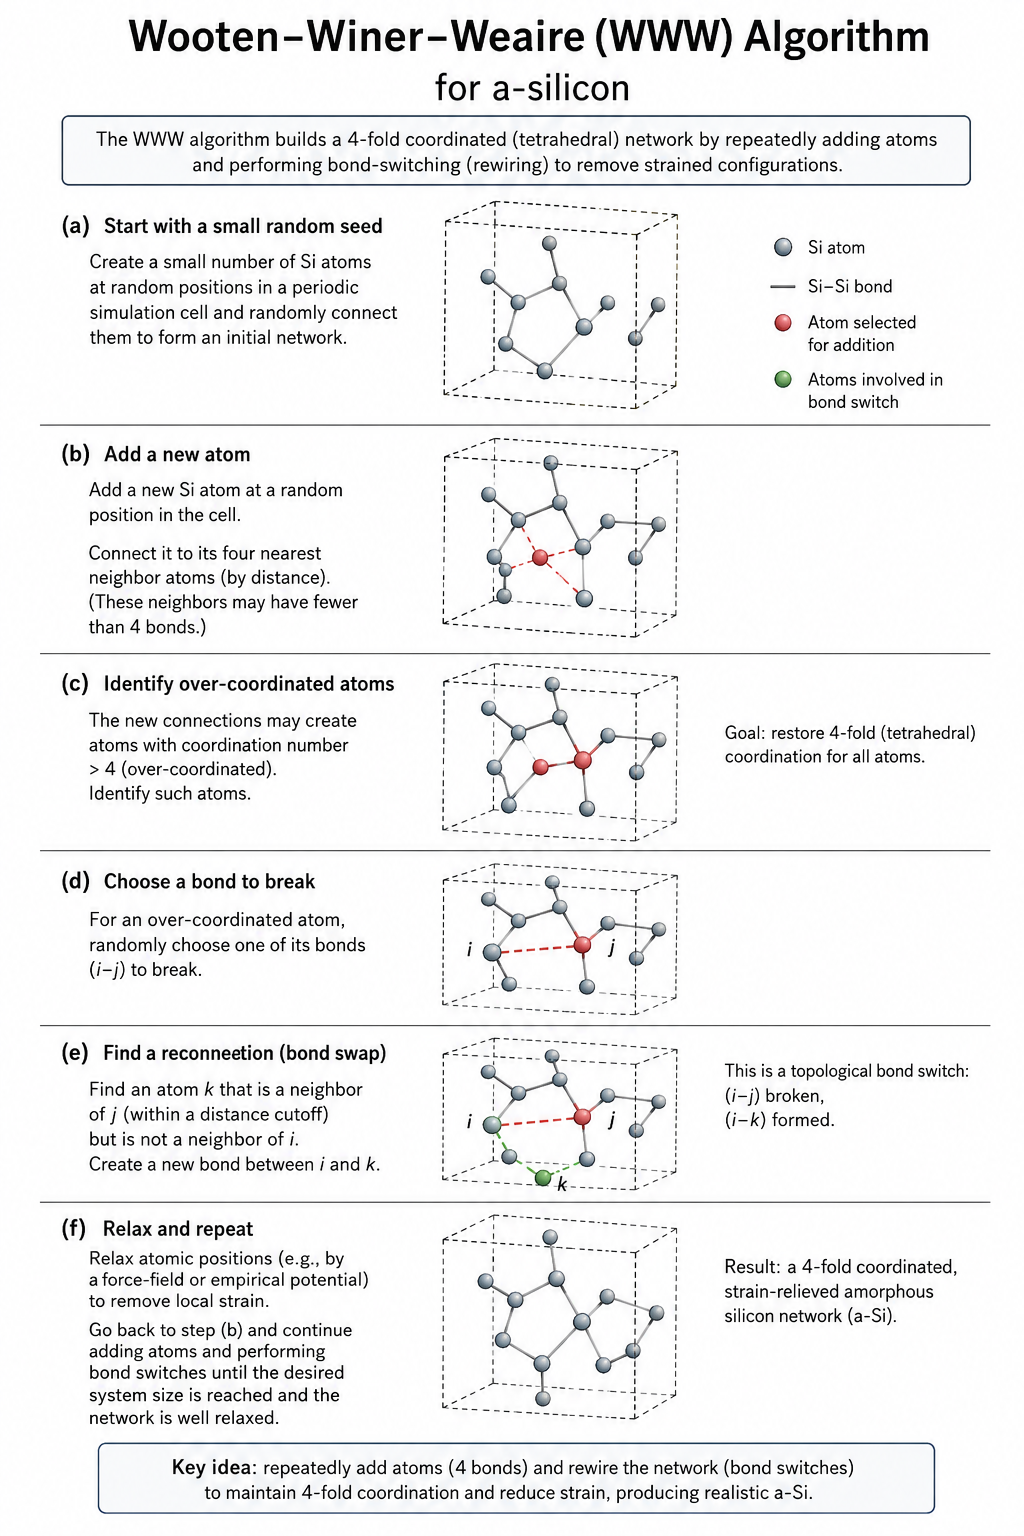
\includegraphics[width=0.8\textwidth]{Wooten-Winer-Weaire.png}
    \caption{Schematic of the Wooten-Winer-Weaire (WWW) algorithm for generating continuous random network models of a-Si.}
    \label{fig:WWW_algorithm}
\end{figure}

In an ideal CRN, every atom remains fourfold coordinated, but long-range periodic order is lost. Bond lengths stay tightly clustered near the crystalline value, while bond angles are spread around the tetrahedral angle of $109.47^\circ$ (typically with a root-mean-square spread on the order of $10^\circ$). The dihedral angles\footnote{Dihedral angles are the angles between two planes, in this case the planes formed by the atoms in the molecular structure.} become essentially random. This is the key difference from perfectly periodic c-Si, where both bond lengths and angles take sharp fixed values.

\subsubsection{Coordination Defects}
\begin{definition}[Coordination Defect]
    \label{C.D}
    A coordination defect in a-Si is an atom that deviates from the ideal fourfold coordination, such as a dangling bond (threefold) or a floating bond (fivefold).    
\end{definition}
\begin{definition}[Dangling Bond]
    A dangling bond is an unsatisfied chemical bond on an atom that is fixed in place. It occurs when an atom is missing one of its expected neighbors, leaving an unpaired electron. This makes the site chemically very reactive and can also create local magnetic moments and signals in electron spin resonance (ESR).
\end{definition}
\begin{definition}[Floating Bond]
    A floating bond is a conceptual defect in covalent networks where an atom is over-coordinated. Floating bonds delocalize their excess charge, allowing the network to remain locally flexible without introducing strong magnetic moments. It possesses an extra paired or mobile electron within the lattice which can contribute to electrical conductivity and influence the material's electronic properties.
\end{definition}

Crucially, the concentration of coordination defects is not intrinsic to a-Si but depends strongly on sample preparation. Experimentally, as-implanted a-Si is highly defective and strained, but these defects anneal out under thermal relaxation as the network relaxes toward a lower-energy state. The same sensitivity appears in simulation: melt-quench MD traps coordination defects, increasingly so at faster quench\footnote{Quench is rapid cooling.} rates, whereas WWW bond-switching relaxes toward near-perfect fourfold coordination. Reverse Monte Carlo (RMC), the activation-relaxation technique (ARTn), and force-enhanced atomic refinement (FEAR) each strike a different balance between matching experimental data and minimizing defect density.

\subsubsection{Ring Defects and Medium-Range Order}
\begin{definition}[Ring in a Network]
    A ring is a closed loop of bonds connecting atoms, like following bonds from atom to atom until you return to the starting point.
\end{definition}
\begin{definition}[Ring Defect]
    Ring defects describe how these loops vary in size in a-Si. In c-Si, every loop contains exactly six atoms (a six-membered ring). In a-Si, most rings are still six-membered, but many are not. The most important are five- and seven-membered rings, which correspond to loops that are either too small or too stretched compared to the crystal structure. These distortions create local strain, change bond angles, and can introduce electronic gap states.
\end{definition}

\begin{definition}[Medium-Range Order]
    %A ring defect is a specific structural feature that refers to one identifiable loop in the atomic network. Medium-range order (MRO) is a broader description of how structured the material is over distances beyond nearest neighbors, capturing patterns and correlations over a few atomic spacings.
    Medium-range order (MRO) refers to structure that persists beyond nearest neighbors, over a few atomic spacings, without extending to the long-range periodicity of a crystal. In a-Si it appears in ring statistics, where certain ring sizes (especially 5-, 6-, and 7-membered) occur preferentially, and in recurring local motifs or clusters that influence the material's properties.
\end{definition}

In realistic a-Si models the ring distribution peaks around five-, six-, and seven-membered rings. Three-membered rings are essentially absent, and four-membered rings are rare because both are heavily strained\footnote{The bonds are forced into shapes they don't want to be in, so they store energy and are unstable, like a bent spring that wants to snap back.}.

One practical caveat is that there is no single agreed-upon rule for what counts as a ``ring'' in a disordered network. Several definitions exist (King or shortest-path, Guttman, and primitive rings), and each can count the loops in the same structure differently. As a result, the reported ring distribution always depends on which counting method was used, and the two must be interpreted together.


\subsubsection{Applications}
a-Si is used predominantly as a semiconductor for large-area and flexible electronics. Because it can be deposited on inexpensive, flexible substrates at low temperatures. Its major commercial and industrial applications include:

\begin{itemize}
    \item \textbf{Active-matrix displays.} a-Si is the foundational material for the thin-film transistor (TFT) arrays in liquid-crystal displays (LCDs), controlling individual pixels in laptops and televisions.
    \item \textbf{Photovoltaics and solar power.} It is used in lightweight, flexible, and semi-transparent thin-film solar panels. Although less efficient than c-Si, a-Si panels perform well in low-light conditions.
    \item \textbf{Medical X-ray imaging.} In large-area digital X-ray flat-panel detectors, a-Si arrays convert X-rays into high-resolution digital images.
    \item \textbf{Sensors and scanners.} a-Si is deployed in document scanners, electronic whiteboards, and optical colour sensors because it can cover large surface areas.
    \item \textbf{Gravitational wave detectors} Like LIGO\footnote{Laser Interferometer Gravitational-Wave Observatory.} use a-Si coatings on mirrors to reduce thermal noise and improve sensitivity.
    \item \textbf{Quantum computers} Use a-Si in superconducting qubits and Josephson junctions\footnote{Josephson junctions are weak links between two superconductors that allow for the flow of Cooper pairs.}, where its low defect density and tunable properties help maintain coherence.
\end{itemize}

\subsubsection{The Paracrystallinity Debate}
A long-standing debate concerns whether a-Si is genuinely a pure continuous random network, or whether real samples contain small ordered regions mixed into the disordered matrix. The two competing pictures are:

\begin{itemize}
    \item \textbf{Continuous random network (CRN):} a-Si has no long-range repeating pattern, and nearly every atom is fourfold-coordinated in a disordered network shaped only by its local tetrahedral geometry.
    \item \textbf{Paracrystalline model:} a-Si contains small, crystal-like regions of local order (``paracrystallites'') surrounded by disordered material, so the structure is not fully random at the medium range.
\end{itemize}

Support for the paracrystalline picture comes from fluctuation electron microscopy (FEM), a technique that can pick up medium-range order which ordinary diffraction tends to average away. Treacy and Borisenko (2012)~\cite{treacy2012} read their FEM signals as evidence for tiny paracrystalline regions. This reading was questioned by others, and the issue stayed unresolved because the measurement is indirect rather than a direct image of the structure. More recently, the debate has reopened from the simulation side, Rosset, Drabold and Deringer (2025)~\cite{rosset2025} find paracrystalline order appearing in large machine-learning MD models of a-Si, suggesting that the pure CRN may not fully describe real samples.

\begin{figure}[H]
    \centering
    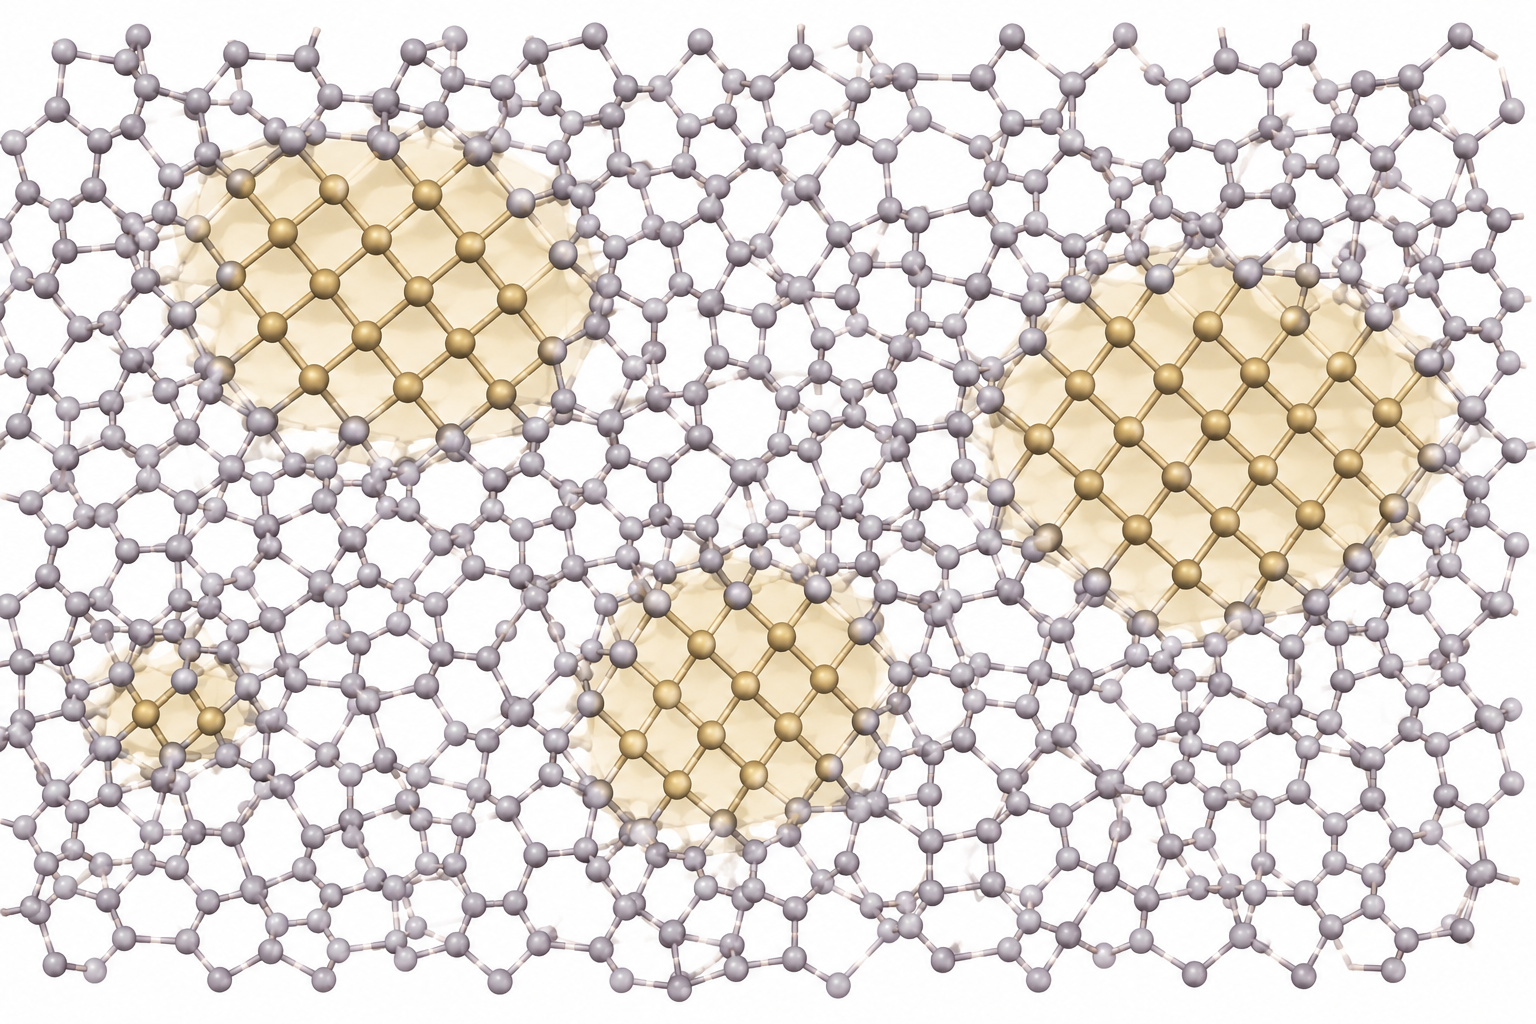
\includegraphics[width=0.8\textwidth]{paracrystallinity.png}
    \caption{Schematic illustration of the paracrystalline model of a-Si. Small crystal-like regions (paracrystallites) with short- to medium-range order are embedded within an otherwise disordered continuous random network. The highlighted ordered domains are illustrative and are not drawn to scale.}
    \label{fig:paracrystallinity}
\end{figure}


\subsection{Structural and Dynamical Characterization}
\label{sec:metrics}

A simulation produces nothing but a list of atomic positions at each timestep. Deciding whether that list represents a crystal, a liquid, or an amorphous solid requires reducing it to a small number of quantities that distinguish the three phases. Four are used in this project: the radial distribution function, the coordination number, the mean square displacement, and the tetrahedral order parameter. The first two describe structure, the third describes dynamics, and the fourth measures local geometry directly.

\subsubsection{Radial Distribution Function}
\label{RDF}
\begin{definition}[Radial Distribution Function]
    The radial distribution function (RDF), written $g(r)$\footnote{Incidentally, $g(r)$ doubles as a bridge to two other things: the distance at which its oscillations die out is the correlation length $L_c$ that MAP relies on, and its Fourier transform is the static structure factor $S(q)$ that X-ray and neutron diffraction experiments measure directly.}, gives the probability of finding an atom at a distance $r$ from a reference atom, normalized by the probability expected for a uniform system of the same average density.
\end{definition}
A value $g(r) = 1$ means the local density at that separation equals the bulk average, the material has lost all local structure (completely random distribution), $g(r) > 1$ means atoms preferentially sit at that distance, and $g(r) = 0$ means that separation never occurs, since atoms are too close and their electron clouds overlap.

Formally, for a system of $N$ atoms at number density $\rho = N/V$,
\begin{equation}
    g(r) = \frac{1}{4\pi r^{2}\, \rho N} \left\langle \sum_{i=1}^{N} \sum_{j \neq i} \delta\!\left(r - r_{ij}\right) \right\rangle,
    \label{eq:rdf}
\end{equation}
where $r_{ij}$ is the separation between atoms $i$ and $j$, the angle brackets denote a time average over the trajectory, and the factor $4\pi r^{2}$ is the surface area of the spherical shell at radius $r$. Dividing by this shell area is what converts a raw count of neighbours into a density, since a shell far from the reference atom is larger and would otherwise contain more atoms purely for geometric reasons.

The shape of $g(r)$ is the primary structural fingerprint of a phase:
\begin{itemize}
    \item \textbf{Crystalline silicon.} Sharp, well-separated peaks at the discrete neighbour shells of the diamond lattice (2.35, 3.84, 4.50~\AA), dropping to zero between them and persisting undamped to arbitrarily large $r$. That persistence is what long-range order means.
    \item \textbf{Liquid silicon.} A single broad first peak near 2.45~\AA, a weak smeared second peak near 3.8~\AA, and nothing beyond: the oscillations damp to $g(r) \to 1$ within a few angstroms.
    \item \textbf{Amorphous silicon.} Intermediate. The first peak stays sharp at 2.35~\AA{} and a distinct second peak survives at 3.84~\AA, since the tetrahedral angle of $109.47^\circ$ is preserved locally, but the third is weak or absent and $g(r) \to 1$ beyond roughly 7 to 8~\AA. Keeping the second peak while losing the third is what separates an amorphous network from a liquid.
\end{itemize}

\subsubsection{Coordination Number}
\label{CN}
\begin{definition}[Coordination Number]
    The coordination number is the average number of nearest neighbours per atom, obtained by integrating the radial distribution function over the first neighbour shell.
\end{definition}

The running coordination number follows from $g(r)$ by integration,
\begin{equation}
    n(r) = 4\pi \rho \int_{0}^{r} g(r')\, r'^{2}\, \mathrm{d}r',
    \label{eq:coord}
\end{equation}
and the coordination number proper is $n(r_{\text{cut}})$ evaluated at the first minimum of $g(r)$, which is the natural boundary between the first and second neighbour shells. For silicon this cutoff is conventionally taken as 2.85~\AA, the value used by Zongo et al.~\cite{zongo2025} in their OVITO coordination analysis.

In c-Si the coordination number is exactly 4 by construction. In a-Si it remains close to 4, and the deviation from it is the coordination-defect concentration discussed in Section~\ref{C.D}: threefold atoms are dangling bonds, fivefold atoms are floating bonds. In liquid silicon it rises to roughly 6, because melting destroys the directional covalent bonding and the liquid adopts a denser, more metallic packing. This same change is what makes liquid silicon denser than the crystal ($2.57$ against $2.33$~g/cm$^3$), an anomaly shared with water and one that provides an independent thermodynamic check on melting: under NPT the volume should contract, not expand, when the crystal melts.

\subsubsection{Mean Square Displacement}
\label{MSD}
\begin{definition}[Mean Square Displacement]
    The mean square displacement (MSD) measures how far atoms have travelled from their initial positions, averaged over all atoms:
    \begin{equation}
        \text{MSD}(t) = \frac{1}{N}\sum_{i=1}^{N} \left\langle \left| \mathbf{r}_i(t) - \mathbf{r}_i(0) \right|^{2} \right\rangle.
        \label{eq:msd}
    \end{equation}
\end{definition}

Unlike $g(r)$ and the coordination number, which are static and computed from a single configuration, the MSD is a dynamical quantity and requires a trajectory. It separates solids from liquids unambiguously:
\begin{itemize}
    \item \textbf{Solid.} Atoms vibrate about fixed lattice sites, so the MSD rises briefly and then plateaus at a small value of order $0.1$~\AA$^2$, set by the thermal vibration amplitude. The plateau grows with temperature but never becomes unbounded.
    \item \textbf{Liquid.} Atoms diffuse without restriction, so after a short ballistic transient the MSD grows linearly and without bound. The slope gives the self-diffusion coefficient through the Einstein relation,
    \begin{equation}
        D = \lim_{t \to \infty} \frac{\text{MSD}(t)}{6t},
        \label{eq:einstein}
    \end{equation}
    where the factor 6 is $2d$ for $d = 3$ dimensions.
\end{itemize}

A linear, unbounded MSD is the single most direct confirmation that a crystal has melted, since it demonstrates the atoms are genuinely diffusing rather than vibrating in place.

\subsubsection{Tetrahedral Order Parameter}
\label{TOP}
\begin{definition}[Tetrahedral Order Parameter]
    The tetrahedral order parameter $q$ measures how closely an atom's four
    nearest neighbours approach ideal tetrahedral geometry~\cite{chau1998,errington2001}:
    \begin{equation}
        q = 1 - \frac{3}{8}\sum_{j=1}^{3}\sum_{k=j+1}^{4}
            \left( \cos\theta_{jk} + \frac{1}{3} \right)^{2},
        \label{eq:tetra}
    \end{equation}
    where $\theta_{jk}$ is the angle subtended at the central atom by neighbours $j$ and $k$. The double sum runs over all six distinct neighbour pairs.
\end{definition}

Both constants follow from the geometry. In a perfect tetrahedron every pair of bonds subtends the same angle $\theta = 109.47^\circ$, for which $\cos\theta = -1/3$; each bracket therefore vanishes and $q = 1$ exactly. The prefactor $3/8$ is fixed by requiring the opposite limit to give zero. For randomly oriented neighbours $\langle\cos\theta\rangle = 0$ and $\langle\cos^{2}\theta\rangle = 1/3$, so
\begin{equation}
    \left\langle \left(\cos\theta + \tfrac{1}{3}\right)^{2} \right\rangle = \left\langle \cos^{2}\theta \right\rangle + \tfrac{2}{3}\left\langle \cos\theta \right\rangle + \tfrac{1}{9} = \tfrac{1}{3} + 0 + \tfrac{1}{9} = \tfrac{4}{9},
\end{equation}
and summing over the six pairs gives $6 \times \tfrac{4}{9} = \tfrac{8}{3}$. Multiplying by $3/8$ returns unity, so $\langle q \rangle = 0$. The parameter therefore runs from $1$ for ideal tetrahedral order to $0$ for a structureless arrangement, with no reference table required. This normalization matches that used by Zhao et al.~\cite{zhao2017}, who applied $q$ to \textit{ab initio} molecular dynamics of liquid silicon.

Crystalline silicon sits at $q = 1$ by construction. Amorphous silicon falls slightly below it, since the network preserves fourfold coordination while broadening the bond-angle distribution. Liquid silicon falls further still as the coordination number rises toward six and the tetrahedral geometry is lost entirely.

\subsubsection{Summary of Phase Signatures}

Each metric alone is ambiguous. The radial distribution function of a-Si resembles that of a liquid at short range, the coordination number of a liquid can drift toward four on cooling, and a solid at high temperature can show a large mean square displacement plateau. Melting and amorphisation are therefore identified by the agreement of all four indicators rather than by any one of them.

\begin{table}[H]
\centering
\small
\begin{tabular}{p{0.16\textwidth}|p{0.22\textwidth}|p{0.22\textwidth}|p{0.24\textwidth}}
\toprule
Metric & Crystalline (c-Si) & Liquid Si ($2500$~K) & Amorphous (a-Si) \\
\midrule
$g(r)$, Sec.~\ref{RDF}
    & Sharp peaks persisting undamped to large $r$
    & Broad first peak, weak second, flat beyond
    & Sharp first and second peaks, third weak or absent \\
\hline
Coordination number, Sec.~\ref{CN}
    & $4$ exactly
    & $\approx 6$
    & $\approx 4$, defects below a few \% \\
\hline
MSD, Sec.~\ref{MSD}
    & Plateaus, order $0.1$~\AA$^2$
    & Linear and unbounded
    & Plateaus \\
\hline
Tetrahedral order $q$, Sec.~\ref{TOP}
    & $1$ by construction
    & Falls toward $0$
    & Slightly below $1$, broadened by bond-angle spread \\
\bottomrule
\end{tabular}
\caption{Signatures distinguishing the three phases of silicon. Melting is confirmed by the agreement of all four rather than by any one alone. The density is not an independent structural metric but follows from the coordination number, and provides a thermodynamic cross-check available directly from the NPT output: melting must contract the box rather than expand it.}
\label{tab:phase_signatures}
\end{table}

Two practical constraints govern how these quantities are computed in this project. First, all four are meaningful only when averaged over a trajectory at a single equilibrated state; averaging across a heating or cooling ramp mixes configurations from different phases into one curve that describes neither. The structural analysis is therefore performed on the isothermal hold runs rather than on the melt or quench ramps. Second, $g(r)$ under periodic boundary conditions is only defined out to half the box length, which for the 216-atom cell used here limits the accessible range to roughly $8$~\AA.

\subsection{Interatomic Potentials}

\subsubsection{Interatomic Potentials in Molecular Dynamics}
\begin{definition}[Molecular Dynamics]
    Molecular dynamics (MD) is a computational method for simulating the physical movements of atoms and molecules.
\end{definition}
\begin{definition}[Force Field]
    A force field is the complete set of functions and fitted parameters used to compute the energy and forces of a system. In practice the terms ``force field'' and ``interatomic potential'' are used interchangeably, though ``force field'' is more common in chemistry and biomolecular simulation, and ``potential'' in materials physics.
\end{definition}

Potentials differ in where their parameters come from, which is the usual way of classifying them:
\begin{itemize}
    \item \textbf{Ab initio} (``from first principles''): the energy is computed directly from quantum mechanics with no parameters fitted to data. DFT is the standard example. Accurate but expensive.
    \item \textbf{Empirical and semi-empirical:} a fixed mathematical form is chosen on physical grounds, and its parameters are then fitted to reproduce known data, either experimental measurements or ab initio calculations. The Lennard-Jones and Stillinger-Weber potentials are of this kind. ``Semi-empirical'' signals that the functional form carries real physics while the numbers inside it are fitted. Cheap, but limited by the rigidity of the chosen form.
    \item \textbf{Machine-learned:} no fixed functional form at all. The relationship between structure and energy is learned from a large set of ab initio reference calculations. MTPs belong here.
\end{itemize}
MD simulations evolve a system of atoms in time by integrating Newton's equations of motion. To do this we need the forces on each atom at every timestep, which means we need a model of the potential energy as a function of atomic positions. This model is the interatomic potential.

\begin{definition}[Interatomic Potential]
    \label{IP}
    An interatomic potential is a mathematical function that describes the potential energy of a system of atoms as a function of their positions. It is used to calculate forces and energies in MD simulations.
\end{definition}

\subsubsection{Lennard-Jones Potential}
\begin{definition}[Lennard-Jones Potential]
    The Lennard-Jones (LJ) potential is a total interaction energy combining an attractive and a repulsive term. The attraction comes from London dispersion forces (instantaneous induced-dipole--induced-dipole interactions), and the repulsion arises from Pauli exclusion when the electron clouds of two atoms overlap at short range.
\end{definition}
The LJ potential is the simplest widely used empirical pair potential:
\begin{equation}
    V_{LJ}(r) = 4\epsilon \left[ \left( \frac{\sigma}{r} \right)^{12} - \left( \frac{\sigma}{r} \right)^{6} \right]
\end{equation}
It has only two free parameters. The distance $\sigma$ is the separation $r$ at which the potential energy crosses zero, that is, where attraction and repulsion exactly cancel. Physically, $\sigma$ acts as the effective diameter of an atom. Two atoms strongly repel once they come closer than about $\sigma$. The lowest-energy separation (the bottom of the well, where the atoms sit at rest) is slightly larger, at $r = 2^{1/6}\sigma$.

The energy $\epsilon$ is the depth of the potential well, how much energy you would have to supply to pull two bonded atoms apart to infinity, which sets how strongly two neighbouring atoms are bound.

Changing $\sigma$ and $\epsilon$ only rescales the curve along the $r$ and $V$ axes respectively; the overall shape stays the same regardless of how they are tuned.
\begin{definition}[Lennard-Jones Substance]
    \label{LJ Substance}
    A Lennard-Jones substance is a material modelled with the Lennard-Jones potential, whose interaction is fixed by only two parameters, $\sigma$ and $\epsilon$. Since these merely rescale the size and depth of the same fixed curve, they set how large and how strongly bound the atoms are, but never change the qualitative nature of the bonding. This restricts the LJ model to systems whose bonding is genuinely simple and isotropic\footnote{The same in all directions, with no preferred bonding angles.}, such as the noble gases.
\end{definition}
Noble gas atoms actually behave the simple way LJ describes: they're basically little spheres that don't care about direction, they just weakly stick and repel when squished. LJ's two knobs are enough to capture them fully. Silicon doesn't work that way, its atoms demand specific bond angles ($109.5^\circ$), and LJ has no knob for angles, so it physically cannot represent silicon no matter how you set $\sigma$ and $\epsilon$.

In general, the higher the desired accuracy of a potential, the more complex the model becomes. More complex models need more free fitting parameters and more expensive force and energy evaluations at runtime. Choosing a potential is a trade-off between physical accuracy and computational cost.

\subsubsection{Other Interatomic Potentials}
Several families of potentials exist beyond LJ, each suited to different bonding environments:
\begin{itemize}
    \item \textbf{Morse potential.} A pair potential for diatomic molecules. More flexible than LJ since it has three parameters and a more realistic anharmonic shape.
    \item \textbf{Stillinger-Weber (SW)}~\cite{sw1985}. Includes explicit three-body terms, well-suited for covalently bonded materials like silicon.
    \item \textbf{Bond order potentials.} Make bond strength depend on the number and type of neighbours. Examples include the Tersoff~\cite{tersoff1988} and Brenner potentials, widely used for carbon-based materials.
    \item \textbf{Embedded Atom Method (EAM)}~\cite{daw1984}. Designed for metals and metal alloys. See the subsection below.
    \item \textbf{Screened Coulomb potentials.} For ionic systems where charge interactions are screened by other charges in the medium. Examples include the Yukawa and Debye-Hückel potentials.
    \item \textbf{Non-parametric / machine learning potentials.} No fixed functional form. The potential is instead learned from data. Examples include Moment Tensor Potentials and neural network potentials. These can capture complex interactions and are increasingly used for materials with non-trivial bonding\footnote{Non-trivial bonding refers to bonding that is not simply pairwise, but involves more complex interactions.} such as a-Si.
\end{itemize}

\subsubsection{Embedded Atom Method}
EAM models energies and forces in metallic systems. The total energy of atom $i$ is:
\begin{equation}
    E_i = F_\alpha\!\left(\sum_{j \neq i} \rho_\beta(r_{ij})\right) + \frac{1}{2}\sum_{j \neq i} \phi_{\alpha\beta}(r_{ij})
\end{equation}
The first term is the embedding function $F_\alpha$ evaluated at the local electron density contributed by all neighbours, and the second is a pair potential $\phi_{\alpha\beta}$ between atoms $i$ and $j$. The embedding term is what makes EAM many-body: an atom's energy depends on the cumulative electron density around it, not just on pairwise distances.
\begin{definition}[Embedding Function]
    $F_\alpha(\rho_i)$ gives the energy cost of embedding an atom in a region of local electron density $\rho_i$.
\end{definition}
\begin{definition}[Local Electron Density]
    The sum $\rho_i = \sum_{j \neq i} \rho_\beta(r_{ij})$ of electron density contributions from all neighbouring atoms at the position of atom $i$.
\end{definition}
\begin{definition}[Pair Potential]
    $\phi_{\alpha\beta}(r_{ij})$ describes the direct interaction energy between atoms $i$ and $j$ as a function of their separation.
\end{definition}

\subsection{Density Functional Theory}
\begin{definition}[Density Functional Theory]
    Density functional theory (DFT) is a quantum-mechanical method for computing the ground-state energy and electronic structure of a system of interacting electrons by treating the electron density, rather than the many-body wavefunction.\footnote{Instead of tracking each electron individually, DFT uses a 3D function $n(\mathbf{r})$ that tells how electrons are distributed in space.}
\end{definition}

The many-electron Schr\"odinger equation is unsolvable for all but the smallest systems, because its wavefunction depends on the positions of every electron at once, so its complexity explodes as electrons are added. DFT sidesteps this by working with the electron density $n(\mathbf{r})$, which describes only how electrons are distributed in space, a function of just 3 coordinates instead of $3N$ for $N$ electrons.

What makes this valid is a result by Hohenberg and Kohn~\cite{hohenberg1964}: the ground-state energy of a system is fully determined by its electron density alone, and the true density is the one that minimizes that energy. In other words, you never actually need the full wavefunction; the density carries all the information, and finding the right density is just an energy-minimization problem.

In practice the density is obtained through the Kohn-Sham scheme~\cite{kohn1965}, which replaces the hard problem of many interacting electrons with an easier one: a set of non-interacting electrons moving in an effective field chosen to reproduce the same density. This swap is not free, however all the complicated physics of how electrons truly interact gets pushed into a single leftover term, the exchange-correlation functional.

\begin{definition}[Exchange-Correlation Functional]
    The exchange-correlation functional $E_{xc}[n]$ collects all the many-body electron interactions (exchange and correlation) not captured by the simpler kinetic and electrostatic terms.\footnote{This is the only part of DFT that is not known exactly and is responsible for most of the error in practical calculations.}
\end{definition}

Since $E_{xc}$ has to be approximated, the accuracy of a DFT calculation depends on how good that approximation is. Two common ones are the local density approximation (LDA), which estimates $E_{xc}$ from the electron density at each point, and the generalized gradient approximation (GGA)~\cite{pbe1996}, which also looks at how quickly the density is changing from point to point.

The problem with DFT is its cost. The amount of computing time grows roughly as the cube of the number of electrons, so doubling the system size makes it about eight times more expensive. This quickly becomes impractical for the long simulations and large atom counts needed to model a-Si. The workaround is to run DFT only on a limited set of atomic arrangements to get accurate reference energies and forces, then train a potential like the MTP to reproduce those results at a tiny fraction of the cost.

% ===========================================================
%  MLIPs
% ===========================================================
\subsection{Machine Learning Interatomic Potentials}
\begin{definition}[Machine Learning Interatomic Potentials]
    Machine learning interatomic potentials (MLIPs) are computational models that use machine learning techniques to predict the potential energy and forces of atomic systems based on training data from high-fidelity calculations.
\end{definition}

% ===========================================================
%  MTP
% ===========================================================
\subsection{Moment Tensor Potential}
\begin{definition}[Moment Tensor Potential]
    Moment Tensor Potentials (MTPs)~\cite{shapeev2016} is a specific type of MLIP that approximate DFT. Their accuracy can be dialed up in a controlled way, the model is built from a set of mathematical building blocks, and adding more of them makes it more accurate (though slower).
\end{definition}

\subsubsection{Why MTP?}
Empirical potentials (like EAM) are fast but locked into a fixed formula, so their accuracy can only go so far. General machine-learning potentials are flexible but computationally expensive. MTP sits in between:
\begin{itemize}
    \item \textbf{Systematically improvable:} its accuracy can be increased in a controlled way by adding more building-block functions.
    \item \textbf{Physically consistent:} it gives the same energy no matter how the atoms are labelled, rotated, or mirrored, as real physics should.
    \item \textbf{Linear scaling:} the cost grows only in proportion to the number of atoms, because each atom only interacts with those within a fixed local range.
    \item \textbf{Multi-element:} it can handle more than one atom type, with the interactions adjusted per chemical species.
\end{itemize}

\subsubsection{Kokkos-accelerated Moment Tensor Potential}

Until recently, the MTP had no GPU version even though it is widely used and already supports active learning. This limited how fast it could run on modern HPC\footnote{High-Performance Computing (HPC) systems are large computer setups made of many connected machines, using fast CPUs and GPUs to perform very large calculations.}. This matters because modern supercomputers are ``mixed systems'', meaning they combine normal CPUs with GPUs from companies like NVIDIA, AMD, or Intel, and each type of hardware usually needs different programming methods to use efficiently. Meng et al. (2026)~\cite{meng2026} solve this by extending the MTP inside the LAMMPS Kokkos package. 
\begin{definition}[Kokkos]
    Kokkos is a tool that lets one version of the code run on different hardware (CPUs and different GPUs) without rewriting it for each device.
\end{definition}
This is the version used in this project through the Kokkos plugin.

The package provides nine different versions of the method. These come from combining three types of usage with three types of hardware. The three usage types are: 
\begin{itemize}
    \item Normal use (computing energies, forces, and stresses for molecular dynamics).
    \item Configuration-based active learning.
    \item Neighborhood-based active learning.
\end{itemize}
The two active learning modes also check a score called the extrapolation grade every so often to detect when the model is unsure and needs new training data.

The three hardware versions are:
\begin{itemize}
    \item CPU version (improved compared to the older MLIP-3 code).
    \item GPU version for large systems (about 50,000 atoms or more per GPU).
    \item GPU version for smaller systems (about 2000 atoms or more per GPU), called `small'.
\end{itemize}
 
Performance is governed by the MTP ``level,'' which exponentially scales the number of basis functions and hence the cost.

The authors benchmarked weak and strong scaling on Narval, whose CPU nodes each carry two AMD EPYC 7532 processors (32 cores each) and whose GPU nodes each carry four NVIDIA A100 SXM4 (40 GB) cards. The optimized CPU variant reaches up to a $2\times$ speedup over MLIP-3, while the GPU variants deliver much larger gains and scale efficiently to million-atom systems.

To stay within GPU memory, the GPU implementations use a chunksize parameter that splits atom processing into reusable chunks, allowing larger systems at similar throughput.

The authors stress that throughput\footnote{the rate at which a system successfully produces, processes, or delivers data over a specific period of time} depends heavily on the hardware, the material, and the simulation conditions. They therefore recommend short single-GPU trial runs of both GPU variants, since the crossover at which the thread-parallel variant overtakes the block-parallel one shifts with atom count, MTP level, and hardware.


% ===========================================================
%  ARTn
% ===========================================================
\subsection{Activation Relaxation Technique Nouveau}
\begin{definition}[Activation Relaxation Technique Nouveau]
    Activation Relaxation Technique nouveau (ARTn)~\cite{barkema1996} is a saddle-point search algorithm used to map the potential energy surface (PES)\footnote{Picture a landscape where height = how much energy a given atom arrangement has. Low valleys = stable arrangements, hilltops = unstable ones. To get from one stable arrangement to another, the atoms must pass through a higher-energy "in-between" state, that's the hill.} and identify transitions between local minima. It explicitly climbs out of a minimum, finds a nearby saddle, and relaxes into a new minimum, allowing for efficient exploration of the energy landscape.
\end{definition}
Unlike straight MD, which has to wait for thermal fluctuations to drive a barrier crossing, ARTn explicitly climbs out of a minimum, finds a nearby saddle, and relaxes into a new minimum. It does this in three phases.

\subsubsection{Activation}
Starting at a local energy minimum, the system is pushed in a random direction. After each push the lowest eigenvalue of the Hessian is checked (using the Lanczos algorithm, which only needs force differences and never builds the full Hessian). As long as this eigenvalue stays positive, the system is still inside the basin of the minimum, so it keeps pushing. Once the eigenvalue flips negative, a direction of negative curvature has been found, pointing toward a nearby saddle.

\subsubsection{Relaxation}
The system is then moved along the negative-curvature direction while the energy is simultaneously minimized in all perpendicular directions. This converges on a first-order saddle point.

\subsubsection{Falling}
The system is nudged just past the saddle along the unstable direction and relaxed normally, settling into a new local minimum on the other side of the barrier.

\subsubsection{Event Acceptance}
\begin{definition}[Activated Event]
    An activated event is a single transition in which the system leaves one local energy minimum, crosses a saddle point, and settles into another. ``Activated'' refers to the energy input needed to get over the barrier.
\end{definition}

Each completed ARTn cycle (activation, relaxation, falling) proposes one such event, which is then accepted or rejected using the Metropolis criterion:
\begin{equation}
    P_{\text{acc}} = \min\!\left[1, \exp\!\left(-\frac{E_{\text{final}} - E_{\text{initial}}}{T}\right)\right],
\end{equation}
where $E_{\text{initial}}$ and $E_{\text{final}}$ are the energies of the starting and ending minima, and $T$ is an artificial temperature parameter (set to $0.25$~eV in Zongo et al.~\cite{zongo2025}). Any event that lowers the energy is always accepted, since the exponent is then positive and the expression exceeds one. Events that raise the energy are accepted with a probability that falls off exponentially with how much they raise it, which is what allows the search to escape shallow traps rather than becoming stuck in the first minimum it finds. The parameter $T$ controls how permissive this is: a larger value accepts more uphill moves.

This is also what is meant by ARTn ``capturing rare events''. In ordinary molecular dynamics, a barrier crossing only happens when a thermal fluctuation is large enough to push the system over, so high barriers are crossed very infrequently and may not be observed at all within an accessible simulation time. ARTn does not wait for such a fluctuation; it constructs a barrier crossing deliberately at every step, and so samples transitions that MD would effectively never reach.

\subsubsection{ARTn-MTP Models of Amorphous Silicon}

Zongo et al. (2025)~\cite{zongo2025} is the central benchmark study for this project. It combines ARTn with the unified Si/O/SiO\textsubscript{2} MTP of Zongo et al. (2024)~\cite{zongo2024} to build seven a-Si models, ranging from 216 to 4096 atoms, and compares them against melt-quench MD using the same potential, as well as against experimental data and other high-quality models from the literature. One important point is that the MTP training set contained no a-Si configurations, so these simulations also test how well the potential transfers to the amorphous phase.

Most models were built by randomly filling a simulation box at a fixed density (2.20 or 2.28 g/cm$^3$) and relaxing it with ARTn. Here ARTn acts as an energy minimizer that escapes local traps by climbing through saddle points, using an artificial temperature parameter (0.25 eV) that controls which structural changes it accepts. The starting configurations were very defective (around 70\% of atoms had the wrong number of bonds in several models), but the final ARTn-MTP structures brought defect levels below 2\%, apart from the 1000-R and 4096-R-MD models at roughly 3\%. The 216-R2 model reached 100\% fourfold coordination, which the authors note is rarely seen outside a handful of Keating-potential WWW models.

Structural quality was checked with standard structural-analysis tools (OVITO~\cite{ovito}, the R.I.N.G.S code~\cite{rings}, and ISAACS), along with LAMMPS pseudosimulations\footnote{Pseudosimulation is a computational technique that mimics the behavior of a real system using simplified models.} for the radial and angular distributions\footnote{OVITO was used for coordination analysis with a 2.85 Angstrom bond cutoff, R.I.N.G.S for ring statistics using the King criterion, and ISAACS for the structure factor.}. The results match experiment and the 100{,}000-atom 100k-GAP18 reference model~\cite{deringer2018} closely: bond angles centre on the tetrahedral value of $109.5^\circ$ with a spread near $10^\circ$, and ring statistics peak at 5-, 6-, and 7-membered rings, with no 3-membered rings and very few 4-membered rings.

The mechanical and energetic properties agree just as well. The bulk modulus averages about 75 GPa across all models, well below the 98.3 GPa of c-Si, matching the softer nature of a-Si. The excess energy (how far above c-Si's energy each model sits) averages 0.167 eV/atom for the ARTn-MTP models versus 0.191 eV/atom for the MD-generated ones, both inside the experimental window of 0.135 to 0.205 eV/atom.

Crystallinity was measured with the ``identify diamond structure'' modifier in OVITO, which flags atoms sitting in cubic or hexagonal diamond environments. Four models (216-R1, 512-R1, 512-R2, and 1000-R) showed zero crystallinity, and all four were generated from a random start with no MD prerun. From the full dataset the authors draw three trends: crystallinity depends little on system size; starting from a random state gives less crystallinity than starting from a melt-and-quench state\footnote{A melt-and-quench state is a simulation technique where a material is first heated to a liquid state and then rapidly cooled to form an amorphous structure.}; and fewer coordination defects tend to go with higher crystallinity.

The main conclusion is that ARTn-MTP produces a-Si with both low crystallinity and low coordination defects, while MD melt-quench tends to trap crystalline grains. This makes ARTn-MTP the better route to near-ideal CRN structures.

\subsection{Morphological Autoregressive Protocol}

\subsubsection{The MAP Framework}

\begin{definition}[Morphological Autoregressive Protocol]
    The Morphological Autoregressive Protocol (MAP), introduced by Madanchi et al. (2024)~\cite{madanchi2024}, is a generative machine-learning method that builds large models of disordered matter (such as glasses or amorphous solids) while keeping the computational cost proportional to the system size, rather than exploding as it grows.
\end{definition}

Conventional simulations of amorphous systems run into an ``exponential wall'': as you add more atoms, the number of possible arrangements (and the amount of sampling needed to explore them) blows up exponentially. MAP gets around this for any material whose structure only ``remembers'' its surroundings over a short distance.

The core idea is to chop the structure onto a grid and build it up one point at a time, like generating a sequence word by word (this is what ``autoregressive'' means). For each grid point, the model learns the probability that it is occupied by a particular atom type, based only on the points already placed nearby. In a disordered material, the influence of one atom on another fades out past a finite correlation length $L_c$, so you only ever need to look at the local neighbourhood rather than the whole system:
\begin{equation}
    P(X_i = \theta \mid \{X_{j<i}\}) = \mathcal{N}\!\left[c_{b,\theta} + F_\theta\!\left(\{X_j \in L_c\}\right)\right],
\end{equation}
where $X_i$ is the grid point being filled, $\theta$ is the atom type, and $\mathcal{N}$ is a softmax that just turns the model's raw scores into probabilities that add up to one across the possible atom types. To build a full structure, you sample this distribution one grid point at a time, feeding each new point back in as context for the next. This lets a small training sample be extended to any size, at a cost that grows only linearly with the number of grid points. The correlation length $L_c$ itself is read off from the radial distribution function.

The function $F_\theta$ is learned using a PixelCNN, a type of neural network that uses ``masked'' filters so that each grid point can only see neighbours that were already generated, never future ones. Masking on its own leaves a ``blind spot'' where some nearby points get ignored. The authors fix this by splitting the 3D filter into separate depth, vertical, and horizontal passes that each feed information in only one direction. This work extends an earlier 2D, single-element version of the method (Kilgour et al., 2020~\cite{kilgour2020}) to 3D with multiple atom types. The important guarantee is that repeatedly generating structures this way forms a Markov chain\footnote{a sequence of states where each one depends only on the last.} that settles onto a single steady distribution equal to the training data. That is what makes the generated structures physically meaningful instead of random noise.

The method is tested on liquid water, with the model trained on path-integral MD data that includes nuclear quantum effects. The generated samples correctly reproduce the O-O, H-H, and O-H radial distribution functions, as well as the H-O-H bond-angle and O-H bond-length distributions. MAP can also be steered to generate structures built around a chosen local motif (either a rare low-density one or a common one), and the match to the reference is tracked using the $q_4$ and $q_6$ Steinhardt bond-order parameters, which are standard numbers for measuring local symmetry, together with their Kullback-Leibler divergence, a measure of how different two distributions are. Finally, structures generated by MAP can be used as starting points for stable, well-behaved MD simulations, confirming that putting the atoms on a grid and generating them this way does not corrupt the physics.

\subsubsection{MAP as an Anomaly Detector}
Madanchi and Simine (2026)~\cite{madanchi2026} take the same trained MAP model and use it in a different way: instead of generating new structures, they use it to study why motion is spread out unevenly in supercooled liquids\footnote{A liquid cooled below its normal freezing point without crystallizing, on its way to becoming a glass.}. The question driving the paper is whether the uneven dynamics of a glass-former (the fact that some regions shuffle around while others stay frozen) can be predicted from a single static snapshot of the structure alone, with no information about motion. Since MAP already knows what a ``normal'' local arrangement looks like compared to the typical equilibrium structure, it can flag unusual arrangements on its own, without ever being told during training which regions actually moved.

The test system is the 80:20 Kob-Andersen mixture, a standard model glass-former (two types of Lennard-Jones particles mixed in a 4-to-1 ratio). The authors first confirm that the model still reproduces structures faithfully, by checking that it matches how particle positions correlate with distance and how a known structural length scale changes with temperature, in line with earlier MD results. They then define a simple per-particle score $\Omega$, the average of six probabilities, one for each of six copies of the particle's surroundings $C_i$ obtained by rotating the sample:
\begin{equation}
    \Omega_j = \frac{1}{6}\sum_{i=1}^{6} p(\mathbf{r} \mid C_i).
\end{equation}
A low $\Omega$ means the particle sits in an unusual, unlikely arrangement, a sign that it is about to rearrange or is rearranging right now. A high $\Omega$ means the opposite: it sits in a very typical, stable spot.

The authors then compare $\Omega$ against particle rearrangements identified separately in the MD trajectory\footnote{These rearrangement events are called h-excitations in the paper.}. The temporary dips and bumps in $\Omega$ line up with these events: about 88\% of the rearrangements show up as a dip and the rest as a bump. If the detection thresholds are pushed very close to the baseline, the method becomes extremely sensitive and catches nearly 100\% of the rearrangements, but it then also flags many particles that do not appear to be moving. Rather than discard these, the authors show they actually reflect real activity nearby: these flagged particles tend to have an unusual number of already-moving neighbours, so $\Omega$ is picking up rearrangements happening around the particle, not just in it. MAP therefore gives an interpretable way to spot the structural warning signs of motion without needing any labelled examples, useful both for studying how glasses relax and for catching unusual regions in melt-quench simulations.

\subsection{Thermodynamic Ensembles}
\begin{definition}[Thermodynamic Ensemble]
    A thermodynamic ensemble is the set of macroscopic quantities held fixed during a simulation. The choice of ensemble determines which physical conditions the simulated system is subject to, and therefore which quantities are free to fluctuate.
\end{definition}

Three ensembles are used in this project, named by the quantities they conserve:
\begin{itemize}
    \item \textbf{NVE} (microcanonical): constant number of atoms, volume, and total energy. Newton's equations are integrated with no thermostat, so the system exchanges nothing with its surroundings. Because total energy should be exactly conserved, this ensemble is a useful check on whether the integration is numerically stable.
    \item \textbf{NVT} (canonical): constant number, volume, and temperature. A thermostat exchanges energy with the system to hold the temperature at a target value, while the box stays fixed. This is the standard choice for production runs at a set temperature.
    \item \textbf{NPT} (isothermal-isobaric): constant number, pressure, and temperature. In addition to the thermostat, a barostat allows the box to expand or contract so that the system reaches the target pressure. Since the volume is free to change, this is the ensemble used to find the density a potential actually prefers.
\end{itemize}

The distinction matters in practice because the box size is only a free parameter under NPT. Running NVT at the wrong volume forces the system into a compressed or stretched state, which shows up as a persistent non-zero pressure.

\subsection{Narval}
\begin{definition}[Narval]
    Narval is a general purpose cluster designed for a variety of workloads. Built by Dell Canada and CDW Canada it is located at the École de technologie supérieure in Montreal. The cluster is named in honour of the narwhal, a species of whale which has occasionally been observed in the Gulf of St. Lawrence.
\end{definition}

\subsubsection{Compiling on a Compute Node}
\label{sec:compile}
Compilation\footnote{Compilation is the process of converting source code into an executable program.} is CPU-intensive and should be run on a compute node rather than the shared login node, which is shared and reserved for lightweight tasks. A compute node is requested from the SLURM scheduler with an interactive allocation:
\begin{verbatim}
    salloc --account=ctb-simine --gres=gpu:1 --cpus-per-task=8
    --mem=16G --time=1:00:00
\end{verbatim}
Once the scheduler grants the node (the prompt changes from \texttt{narval1} to a compute node such as \texttt{ng10403}), the required software environment is loaded and the GPU build script is run:

\begin{verbatim}
    cd ~/LMP_MTP
    module load gcc openmpi flexiblas cmake fftw eigen voro++ cuda
    sh ./build-lmp-mtp-gpu.sh
\end{verbatim}
The \texttt{module load} line activates the compiler (\texttt{gcc}), the GPU toolkit (\texttt{CUDA})\footnote{CUDA is a parallel computing platform and programming model developed by NVIDIA}, and supporting math and build libraries, none of which are available until explicitly requested.

\subsubsection{Filesystems and Their Quotas}
\label{sec:filesystems}
Narval exposes several filesystems with different purposes and quotas, and the distinction matters for long production runs. \texttt{/home} is small and backed up; \texttt{/scratch} is large, fast, per-user and \emph{purged} on a fixed retention schedule; \texttt{/project} is the group allocation, shared between all members and quota-limited on both total size and file count; \texttt{/nearline} is tape-backed archival storage. Current usage against quota is reported by \texttt{diskusage\_report}. All production runs in this project were executed from \texttt{/scratch}, with finished configurations copied to \texttt{/project} for retention. The failure discussed in Section~\ref{sec:quench_fail} makes the practical case for this arrangement.

\subsection{LAMMPS}

\begin{definition}[LAMMPS]
    Large-scale Atomic/Molecular Massively Parallel Simulator (LAMMPS)~\cite{plimpton1995,thompson2022}, developed and distributed by Sandia National Laboratories, is an open-source code for classical particle-based materials simulation. It is the molecular dynamics code used in this project, run on a remote computing cluster accessed via SSH (PuTTY).
\end{definition}

\subsubsection{Simulation Workflow}

A LAMMPS run in this project involves three files:
\begin{itemize}
    \item The input script (with `.in', `.melt', and `.lmp' as file extensions) is the recipe written in LAMMPS' command syntax.
    \item The shell script (with `.sh' as its file extension) is a short bash script that launches LAMMPS and feeds it the input script, typically through a line of the form `lmp\_serial -in test.in'\footnote{The word `serial' indicates the run used a single processor core with no parallelism, which is appropriate for a small test case.}.
    \item The log file (log.lammps) is generated automatically by LAMMPS during the run and records the thermodynamic output (temperature, energy, and pressure at each step), along with timing information and any error messages.
\end{itemize}

\subsubsection{Combining LAMMPS with the MTP}

LAMMPS handles the mechanics of a simulation (tracking atomic positions, building neighbour lists, and integrating Newton's equations of motion) but it is agnostic about where the forces come from. The interatomic potential is supplied as a separate, interchangeable module selected through the \texttt{pair\_style} command. Combining LAMMPS with the MTP therefore means installing an MTP pair style into LAMMPS. Once built, the trained potential is used by pointing the input script at the model file, e.g. \texttt{pair\_style mtp model.almtp}: at every timestep, LAMMPS passes each atom's local neighbourhood to the MTP, which returns the energies and forces that LAMMPS then uses to advance the system. The division of labour is clean: the MTP decides how atoms interact, and LAMMPS decides what happens next.

\subsection{WinSCP}

\begin{definition}[WinSCP]
    WinSCP is a free and open-source software (application) for Microsoft Windows. Its main function is secure file transfer between a local and a remote computer.
\end{definition}

When logged in to WinSCP using the login node `narval.alliancecan.ca` and the username and password created through the CCDB website, enter the path `/scratch/your\_username/'. Then you can drag and drop files between your local computer and the Narval cluster. Do not click on the scratch folder in the home menu, since it will load all folders of every Narval user.

\subsection{PuTTY}

\begin{definition}[PuTTY]
    PuTTY is a free and open-source terminal emulator and serial console. It supports various network protocols, including SSH, Telnet, rlogin, and raw socket connections. In this project, PuTTY is used to establish a secure SSH connection to the Narval cluster for remote command-line access.
\end{definition}

PuTTY uses the same login credentials as WinSCP, but instead of dragging and dropping files, it lets you run commands directly on the cluster. It behaves like a standard Linux terminal: you navigate the filesystem, edit files, and launch simulations by typing commands. The typical workflow is to move into your scratch folder, then submit or run a LAMMPS job from there.

\subsubsection{Interactive Jobs}
\begin{definition}[Interactive Job]
    An interactive job is a compute-node session requested through the scheduler with \texttt{salloc}, which drops the user into a live shell on the allocated node instead of running a pre-written script.
\end{definition}

A regular batch job (\texttt{sbatch}) submits a fixed script to the queue and runs unattended; the user only sees the output afterwards. An interactive job instead gives direct command-line access to the compute node for the duration of the allocation, so commands can be typed, tested, and corrected in real time. This makes it the right tool for tasks that require trial and error, such as compiling software, debugging a crashing binary, or checking that modules load correctly, where waiting through the batch queue after every small change would be far too slow. Batch jobs remain preferable for long production runs, since they do not require the user to stay connected. In this project, interactive jobs were used to compile the custom LAMMPS-MTP build on a compute node (Section~\ref{sec:compile}).


\subsection{Visual Molecular Dynamics}

\begin{definition}[Visual Molecular Dynamics]
    Visual Molecular Dynamics (VMD)~\cite{vmd1996} is a molecular visualization program for displaying, animating, and analyzing large biomolecular systems using 3D graphics and built-in scripting.
\end{definition}

In this project, VMD is used to visualize the atomic configurations and trajectories generated by LAMMPS. A practical subtlety is that LAMMPS produces two distinct kinds of output, and VMD loads each differently. A data file (such as \texttt{config.end\_sim}, written by \texttt{write\_data}) stores a single configuration, whereas a trajectory file (such as \texttt{dump.lammpstrj}, written by the \texttt{dump} command) stores many frames. The graphical loader only exposes the trajectory reader, so data files must instead be loaded through the Tk Console using the TopoTools plugin.

Once a structure is loaded, the drawing method is set to VDW so atoms render as spheres, and \texttt{pbc box} draws the periodic simulation cell. For a trajectory, the playback controls in the main VMD window then animate the configuration through all stored frames.



% ===========================================================
%  3. METHODOLOGY
% ===========================================================
\section{Methodology}

\subsection{Toolchain Validation: Lennard-Jones Melt}

Before simulating a-Si, a standard Lennard-Jones (LJ) melt was run on Narval to confirm that the full toolchain (job submission, LAMMPS execution, and output writing) functioned correctly. This is a generic LJ fluid and not a-Si; its only purpose is validation. A line-by-line annotation of the input script is given in Appendix~\ref{InputScript}.

\subsubsection{Output and Validation}
The total energy per atom remained essentially constant at approximately $-4.62$\footnote{Here energy is negative to signify it would cost energy to pull this system apart.} throughout the run. Because the NVE ensemble conserves energy, this constancy confirms that the integration was stable and the simulation parameters were sound. The temperature\footnote{In reduced LJ units, temperature is dimensionless (measured in units of $\epsilon/k_B$).} relaxed from its initial value of $1.44$ to a steady value near $0.70$ as the initial lattice melted and equilibrated. The run completed $10{,}000$ steps on $13{,}500$ atoms in roughly $95$ seconds of wall time, with no dangerous neighbour-list builds reported, confirming a working toolchain.


\subsubsection{VMD visualisation}
The next step was to visualize the completed LJ melt. The trajectory file \texttt{dump.lammpstrj} produced by the run was transferred to the local machine with WinSCP and loaded into VMD, giving a 3D animation of 101 frames (the initial configuration plus one frame per 100 timesteps). The animation shows the initial fcc lattice melting into a disordered fluid, shown in Fig.~\ref{fig:test_in_vmd}.
\begin{figure}[H]
    \centering
    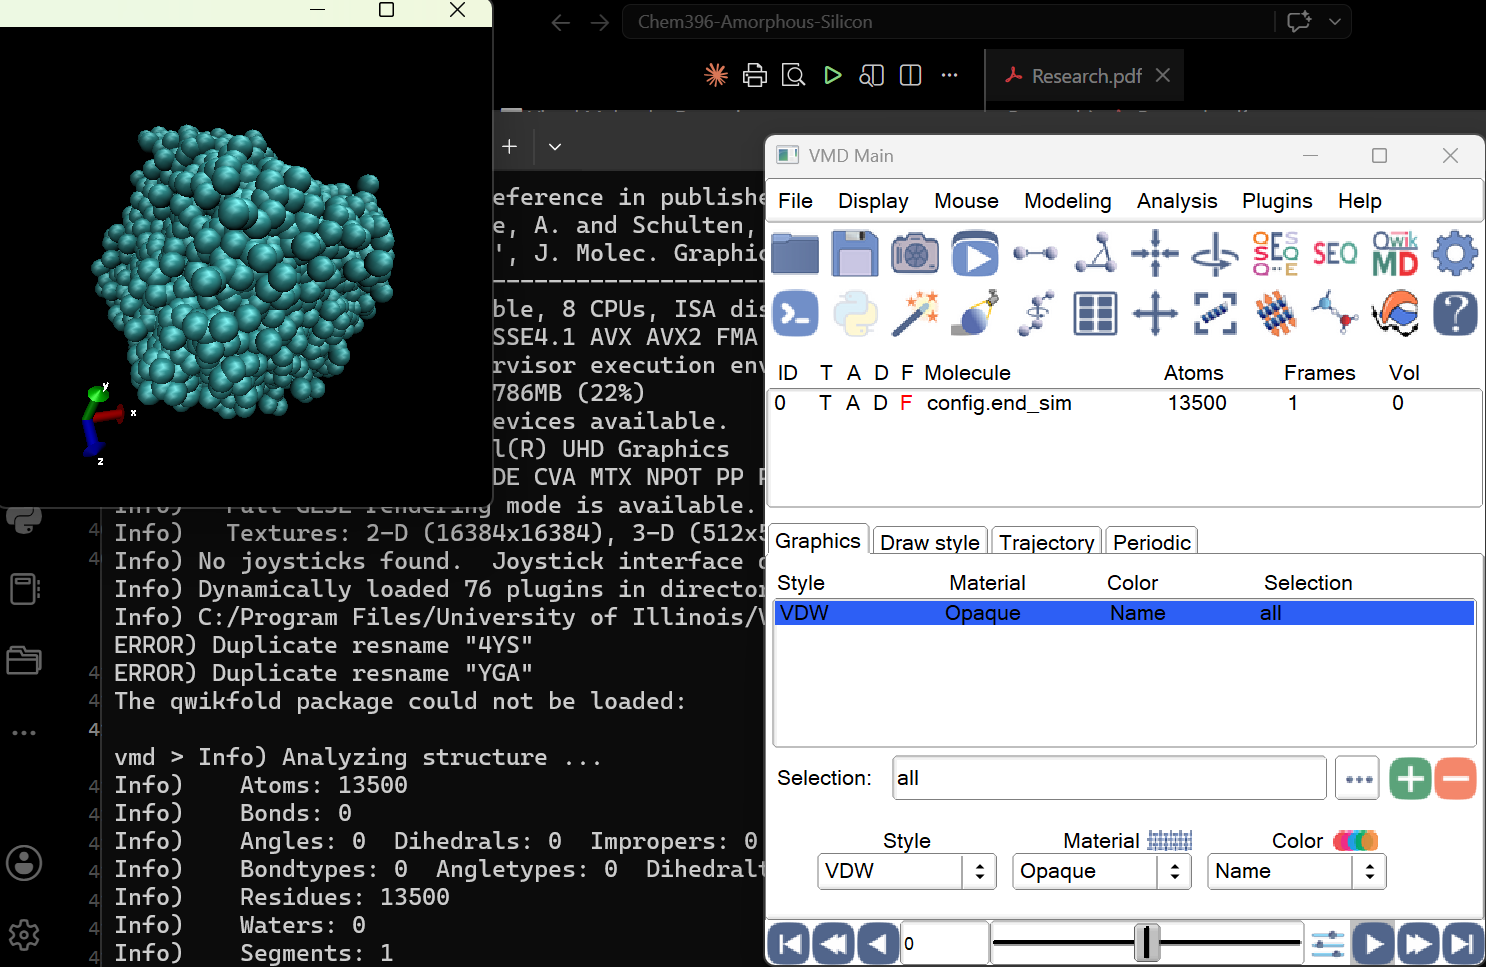
\includegraphics[width=0.8\textwidth]{VMDtestLJSub.png}
    \caption{Visualization of the Lennard-Jones melt simulation in VMD. The atoms are displayed as spheres, and the system has equilibrated into a disordered fluid state.}
    \label{fig:test_in_vmd}
\end{figure}


\subsection{Building LAMMPS with the Moment Tensor Potential}

The Lennard-Jones test used the standard LAMMPS installation already provided on Narval (loaded as a module). Simulating silicon with an MTP instead requires a custom build, because the mtp pair styles are not part of standard LAMMPS. The code was provided by Alliance technical support as an archive, `LMP\_MTP.tar.gz', placed in the home directory. It bundles the LAMMPS source, the MTP source files, and two build scripts: one for a CPU-only build (`build-lmp-mtp-cpu.sh') and one for the GPU (Kokkos) build (`build-lmp-mtp-gpu.sh').

\subsubsection{Debugging the CPU Build}
\marginpar{July 13, 2026}

\begin{table}[H]
\centering
\small
\begin{tabular}{p{0.30\textwidth}|p{0.28\textwidth}|p{0.34\textwidth}}
\toprule
Symptom & Cause & Fix \\
\midrule
Illegal instruction (core dumped) & Binary compiled for a CPU architecture incompatible with Narval's nodes & Add \texttt{-DCMAKE\_CXX\_FLAGS="-march=core-avx2"} \\
\hline
ML-MTP absent from \texttt{lmp -h} & Inverted conditional (\texttt{if [ ! -d ...]}) skipped the source copy & Correct the conditional logic by removing the `!' \\
\hline
Rebuild produced no new binary & Stale nested CMake caches with another user's paths baked in; \texttt{--fresh} resets only the top level & Delete \texttt{\_build} entirely before rebuilding \\
\bottomrule
\end{tabular}
\caption{CPU build faults in the supplied LAMMPS-MTP archive and their fixes.}
\label{tab:buildfaults-cpu}
\end{table}

After a clean rebuild, \texttt{lmp -h} listed \texttt{ML-MTP} with \texttt{mtp} and \texttt{mtp/extrapolation} available as pair styles. Validation was a 10{,}000-step, 13{,}500-atom Lennard-Jones melt submitted through SLURM, completing in 4~min 16~s of wall time with no dangerous neighbour-list builds.

\subsubsection{Debugging the GPU Build}
\marginpar{July 14, 2026}

\begin{table}[H]
\centering
\small
\begin{tabular}{p{0.30\textwidth}|p{0.28\textwidth}|p{0.34\textwidth}}
\toprule
Symptom & Cause & Fix \\
\midrule
\texttt{mtp/kk} styles absent & Script copies only \texttt{ML-MTP}; the \texttt{KOKKOS} folder was never copied & Copy it into \texttt{src/KOKKOS/} \\
\hline
Binary would not run on GPU & Kokkos CUDA backend not enabled & \texttt{kokkos-cuda} preset $+$ \texttt{-DKokkos\_ARCH\_AMPERE80=ON} (A100) \\
\hline
Compilation errors under NVIDIA compiler & \texttt{-march=core-avx2} inherited from the CPU script & Remove the flag \\
\hline
\texttt{GPU} package build failure & OpenCL-based \texttt{-DPKG\_GPU=ON}, redundant alongside Kokkos & Remove the option \\
\bottomrule
\end{tabular}
\caption{GPU (Kokkos) build faults and their fixes.}
\label{tab:buildfaults-gpu}
\end{table}

The GPU build then compiled with \texttt{mtp/kk} and \texttt{mtp/extrapolation/kk} present, and ran the same Lennard-Jones test on an A100 node in $15.6$~s against 4~min 16~s on CPU, a speedup of roughly $16\times$.

\subsection{Simulation Protocol for Amorphous Silicon}
Ata provided five silicon MTPs for this project, split into two groups. Two are melt-stable (levels 22 and 26), fitted explicitly to remain robust at the high temperatures of a melt. The other three are pruned potentials (\texttt{pruned\_1}, \texttt{pruned\_2}, \texttt{pruned\_3}), ordered by increasing computational cost and accuracy, but potentially unstable in a melt. The a-Si is produced by a melt-quench protocol:

\begin{enumerate}
    \item \textbf{Melt.} Heat a c-Si lattice to about 2500~K with a melt-stable potential, and save a snapshot.
    \item \textbf{Hold.} Hold the melt at temperature for 1~ns to erase memory of the crystal.
    \item \textbf{Hand off.} Reload the snapshot with a pruned potential; the atoms are unchanged, only the force model changes.
    \item \textbf{Quench.} Cool from the melt temperature to 300~K, fast enough that the liquid structure freezes in as a-Si rather than recrystallizing.
\end{enumerate}

\subsubsection{Atom Type Mapping}
\marginpar{July 21, 2026}
The potential file declares \texttt{species\_count = 2} without stating which type is which element. This was settled by two NVT runs with potential \texttt{22.almtp} on 216 atoms at 300~K in a fixed box of $4433$~\AA$^3$. Assigning the atoms to type 1 gave a stable run at a density of $2.27$~g/cm$^3$, close to the measured $2.33$~g/cm$^3$ for c-Si. Assigning them to type 2 gave a starting pressure of $-2.24\times10^{6}$~bar and the box collapsed within a few steps into a neighbour-list overflow. Type 1 is therefore silicon and type 2 oxygen, consistent with a potential trained on the Si/O/SiO$_2$ system.

\subsubsection{First Silicon Runs and Choice of Ensemble}
\label{sec:firstruns}
Both ensembles (NVT and NPT) were tested on a 216-atom diamond lattice ($3\times3\times3$ unit cells, $a=5.431$~\AA, periodic, \texttt{units metal}, 1~fs timestep). The intended workflow was NPT equilibration to find the box size the potential prefers, followed by NVT production at that fixed volume.

The protocol was subsequently fixed to NPT only, following Zongo et al.~\cite{zongo2025}, so the NVT stage was dropped. The runs below are retained here as a benchmark of the potentials and of parallel scaling.

The NPT test was run at 300~K and 0~bar and expanded the box from $4325$ to $4433$~\AA$^3$, corresponding to $a=5.476$~\AA. This is $0.8\%$ above the measured value of $5.431$~\AA, an overestimate consistent with the PBE\footnote{Perdew-Burke-Ernzerhof, the generalized gradient approximation exchange-correlation functional used to generate the MTP training data.}~\cite{pbe1996} reference data used to train the potential.

The NVT test was then performed with the lattice rebuilt at $a=5.476$~\AA{}, the volume stayed locked, the pressure settled to order $10^2$--$10^3$~bar rather than the several-thousand-bar swings seen under NPT, and the potential energy showed no drift.

\begin{table}[H]
\centering
\small
\begin{tabular}{l|l|r|r|r}
\toprule
Potential & Ensemble & Cores & Pair time (s) & Wall time \\
\midrule
\texttt{22.almtp}  & NVT & 1 & 1374.7 & 22:55 \\
\texttt{pruned\_1} & NVT & 8 & 12.6   & 00:14 \\
\midrule
\texttt{22.almtp}  & NPT & 1 & 1222.6 & 20:24 \\
\bottomrule
\end{tabular}
\caption{Cost of 5000 steps on 216 atoms. Force evaluation dominates throughout ($\geq 92\%$ of loop time) and no neighbour-list rebuilds occurred in any run.}
\label{tab:firstruns}
\end{table}

\paragraph{The two potentials prefer different volumes.}
An unexpected result came out of the NVT tests. With \texttt{22.almtp}, the pressure at a box volume of $4433$~\AA$^3$ fluctuated around zero, meaning the atoms sit at a spacing that potential is content with. With \texttt{pruned\_1.almtp} in the identical box, the pressure instead held steady at about $-12{,}400$~bar. A negative pressure means the atoms are pulling inward: this potential would prefer a smaller box than the one it has been given.

\subsubsection{Parallel Scaling}
\marginpar{July 22, 2026}
The single-core timings from the previous runs made the cooling stage impractical, so the next step was to find out how much of that cost could be removed.

The same 5000-step NVT run was repeated on 1, 4, and 8 cores of a single node. Running in parallel requires some changes to the submission script, such as launching LAMMPS through \texttt{srun} rather than calling it directly, so that SLURM starts one copy of the program per task and connects them through MPI.


\begin{table}[H]
\centering
\small
\begin{tabular}{l|l|r|r|r|r|r}
\toprule
Potential & Ensemble & Cores & Pair time (s) & Wall time & Speedup & APC\footnote{Atoms per core.} \\
\midrule
\texttt{22.almtp}  & NVT & 1 & 1374.7 & 22:55 & 1.0$\times$ & 216 \\
\texttt{22.almtp}  & NVT & 4 & 305.9  & 05:07 & 4.5$\times$ & 54 \\
\texttt{22.almtp}  & NVT & 8 & 153.8  & 02:43 & 8.4$\times$ & 27 \\
\bottomrule
\end{tabular}
\caption{Wall time for a 5000-step NVT run of 216 silicon atoms using \texttt{22.almtp}, on one node.}
\label{tab:scaling}
\end{table}

The scaling is close to linear up to 8 cores. The limit is nonetheless in sight: the time spent on communication between cores rose from $0.4\%$ of the total at 4 cores to $4\%$ at 8, and with only 27 atoms per core the workload is becoming too thin to divide further. Eight cores was therefore adopted as the default for systems of this size.

\begin{figure}[H]
    \centering
    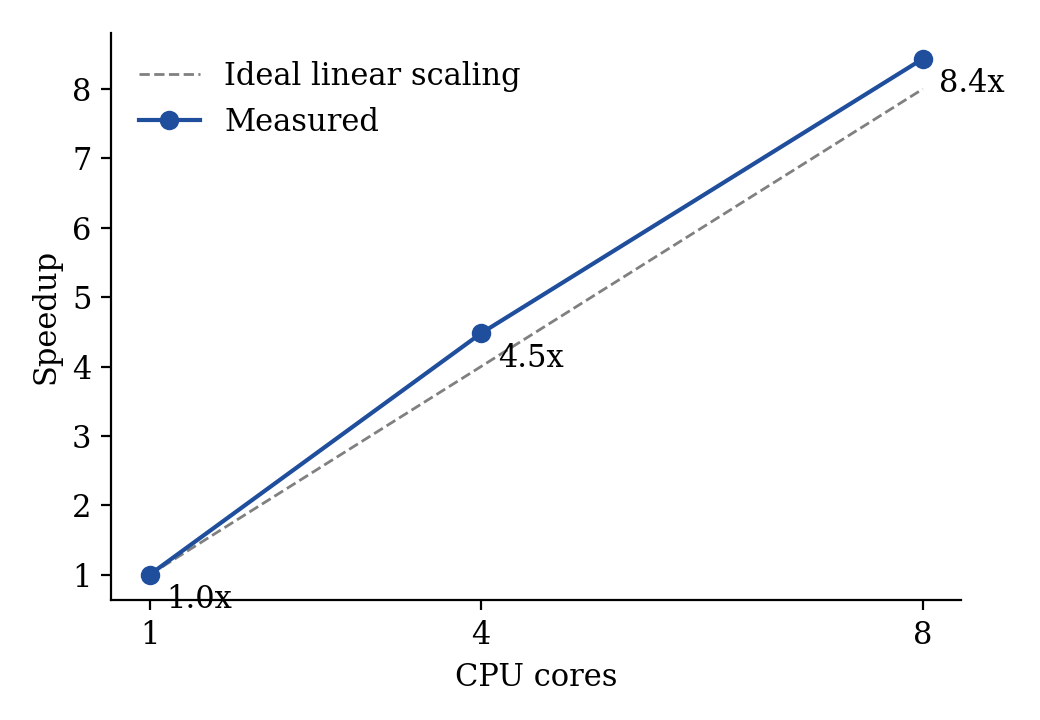
\includegraphics[width=0.6\textwidth]{../report/scaling.png}
    \caption{Parallel speedup of the 5000-step NVT run against the ideal linear case. Scaling is near-linear to 8 cores; the superlinear value at 4 cores likely reflects cache effects at small per-core atom counts.}
    \label{fig:scaling}
\end{figure}


\subsubsection{Setting the Cooling Rate}
\marginpar{July 23, 2026}
A question had to be settled before the melt could be run: how to impose a cooling rate in LAMMPS.

LAMMPS has no command that sets a cooling rate directly. Instead, \texttt{fix npt} takes a starting and a target temperature, and ramps linearly between them over the course of the \texttt{run} that follows. The rate is therefore implied by the length of that run rather than specified:
\begin{equation}
    \text{rate} = \frac{\Delta T}{N_{\text{steps}} \times \Delta t},
\end{equation}
where $\Delta t$ is the timestep and $\Delta T$ the difference in temperature. Using Zongo's cooling rate of 1~K/ps from 2500~K to 300~K, the temperature drop of 2200~K implies 2200~ps of simulated time, which at a 1~fs timestep is $2.2 \times 10^6$ steps.

An immediate consequence, which matters when a run has to be resumed, is that the ramp is defined relative to the current \texttt{run} command and not to any absolute timestep. Restarting a partially completed quench therefore requires the starting temperature and the remaining step count to be recomputed by hand from the point of interruption.

\subsubsection{Projected Cost}
Throughput on 8 cores follows directly from the 5000-step benchmarks of Table~\ref{tab:firstruns} and~\ref{tab:scaling}:
\begin{equation*}
    \texttt{22.almtp}: \; \frac{5000~\text{steps}}{163~\text{s}} = 30.7~\text{steps/s},
    \qquad
    \texttt{pruned\_1}: \; \frac{5000~\text{steps}}{14~\text{s}} = 357~\text{steps/s},
\end{equation*}
where $163$~s and $14$~s are the measured wall times ($2$:$43$ and $0$:$14$). The pruned potential is therefore $357/30.7 \approx 12$ times cheaper per step. At a 1~fs timestep, each stage of the protocol converts to a step count and a wall time as $t_{\text{wall}} = N_{\text{steps}} / r$:

\begin{table}[H]
\centering
\begin{tabular}{l|c|c|c|c}
\toprule
Stage & Potential & Simulated time & Steps & Estimated wall time \\
\midrule
Heating (300--2500~K) & \texttt{22.almtp} & 30~ps & $3.0 \times 10^4$ & 16~min \\
Hold at 2500~K & \texttt{22.almtp} & 1~ns & $1.0 \times 10^6$ & 9.1~h \\
Cooling (1~K/ps) & \texttt{pruned\_1} & 2.2~ns & $2.2 \times 10^6$ & 1.7~h \\
\midrule
Total & & 3.2~ns & $3.2 \times 10^6$ & 11~h \\
\bottomrule
\end{tabular}
\caption{Projected cost of the melt-quench protocol for 216 atoms on 8 cores, using the melt-stable potential for heating and the hold and \texttt{pruned\_1} for cooling. Cooling from 2500~K to 300~K at 1~K/ps fixes the cooling stage at 2200~ps.}
\label{tab:projected_cost}
\end{table}

The hold at 2500~K dominates despite involving less than half the steps of the cooling stage, purely because of the factor of twelve in cost per step. Whether the hold genuinely requires the melt-stable potential, or whether the switch to a pruned one can happen earlier, has been raised with the group. These figures also assume the cost per step stays as measured on a static 300~K crystal; a hot liquid rearranges continuously and will trigger neighbour-list rebuilds that the earlier runs did not (all benchmark runs recorded zero rebuilds), so the true cost will be somewhat higher.


% ===========================================================
%  4. RESULTS
% ===========================================================
\section{Results}
\subsection{Simulation of 216 Amorphous Silicon Atoms}

\subsubsection{Melt P22}
\marginpar{July 24, 2026}
The heating run melted successfully. The temperature reached the 2500~K target, and five signatures confirmed the crystal had become a liquid: 
\begin{itemize}
    \item \textbf{RDF.} Over the last 3~ps, a single broad peak at 2.45~\AA{} damping to $g(r)=1$ by 3.5~\AA. The first 2~ps show the diamond lattice instead: peaks at 2.37, 3.87, 4.54~\AA{} persisting undamped to 8~\AA{} with minima falling to zero between shells.
    \item \textbf{Coordination number.} Counted within a 3.15~\AA{} cutoff, the first minimum of the liquid $g(r)$. The first 2~ps give exactly 4.000 neighbours per atom with 100\% fourfold coordination, as the diamond lattice requires. The final 3~ps give a mean of 5.968, distributed over 3- to 8-fold environments and peaking at sixfold, the denser packing expected once directional covalent bonding is lost.
    \item \textbf{Mean square displacement.} Bounded below $1$~\AA$^2$ for the 25.5~ps, rising slowly from $0.08$ to $0.5$~\AA$^2$ as the thermal vibration amplitude grows with temperature, but never unbounded. At 25.6~ps it turns sharply and grows linearly to $111.4$~\AA$^2$ by the end of the ramp, a factor of 200 in 4.4~ps. Linear unbounded growth is the definitive signature of diffusion, and the transition coincides with the potential-energy jump and volume contraction in the thermodynamic output.
    \item \textbf{Tetrahedral order parameter.} The first 2~ps give $q = 0.9925$ with a standard deviation of $0.0058$, indistinguishable from the ideal value of 1 once thermal vibration is accounted for. The final 3~ps give $q = 0.4977$ with a spread of $0.2046$, a broad distribution reaching from 0 to 1. Roughly half the tetrahedral character is lost, and the collapse of a sharply peaked distribution into a broad one is the local-geometry counterpart of the loss of long-range order seen in $g(r)$.
    \item \textbf{Density.} The box volume averages $4500$~\AA$^3$ over the solid portion of the ramp and $4310$~\AA$^3$ after the transition, giving
    \begin{equation*}
        \rho = \frac{216 \times 28.0855}{6.022 \times 10^{23} \times 4310 \times 10^{-24}} = 2.337~\text{g/cm}^3
    \end{equation*}
    against $2.24$~g/cm$^3$ for the solid, a contraction of $4.2\%$. Silicon is anomalous in that the liquid is denser than the crystal, so a contraction on melting is itself a signature. The absolute values sit below the experimental $2.33$ and $2.57$~g/cm$^3$, consistent with the PBE overestimate of the lattice constant noted by Zongo et al.~\cite{zongo2025}
\end{itemize}
\begin{figure}[H]
    \centering
    \begin{subfigure}{0.48\textwidth}
        \centering
        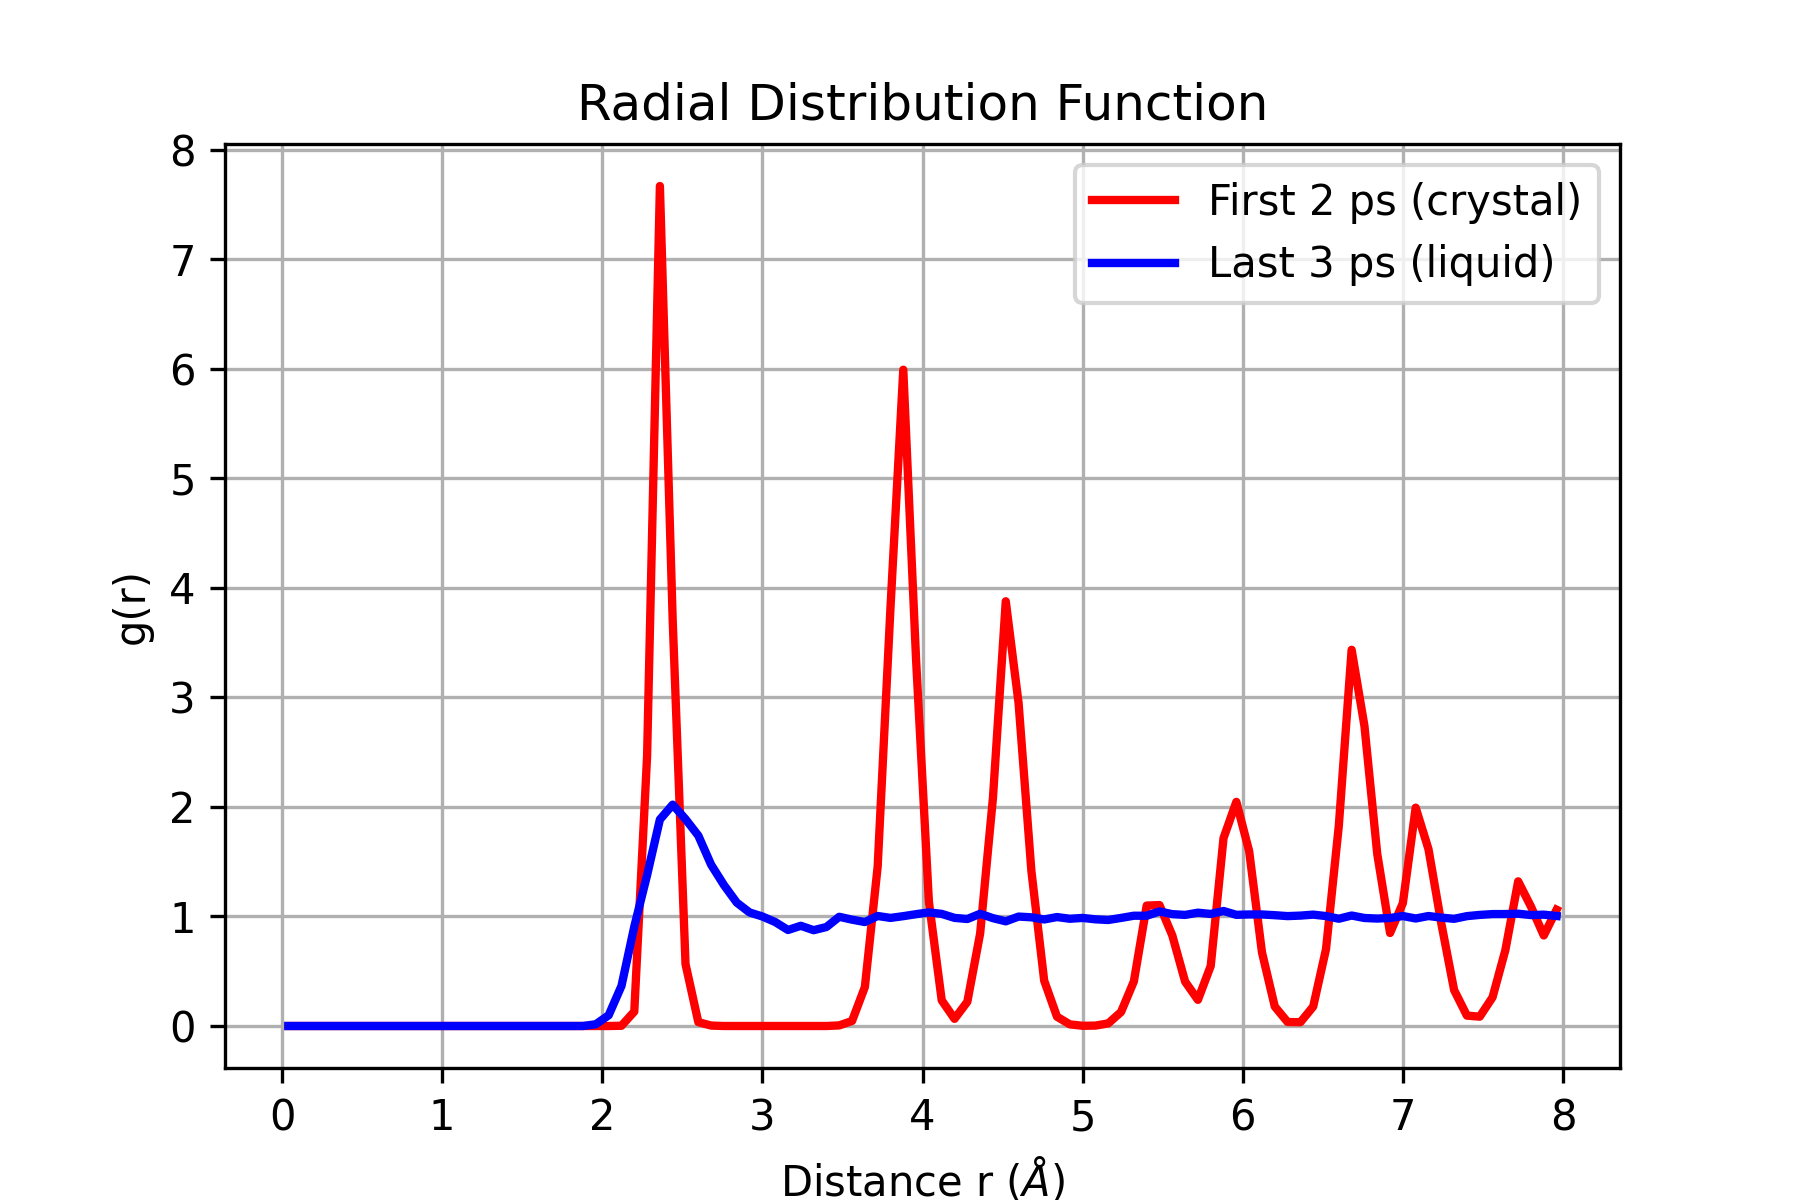
\includegraphics[width=\linewidth]{../python/radial_dist_fct/melt_P22_rdf_output.png}
        \caption{Radial distribution function}
        \label{fig:sfig1}
    \end{subfigure}
    \hfill
    \begin{subfigure}{0.48\textwidth}
        \centering
        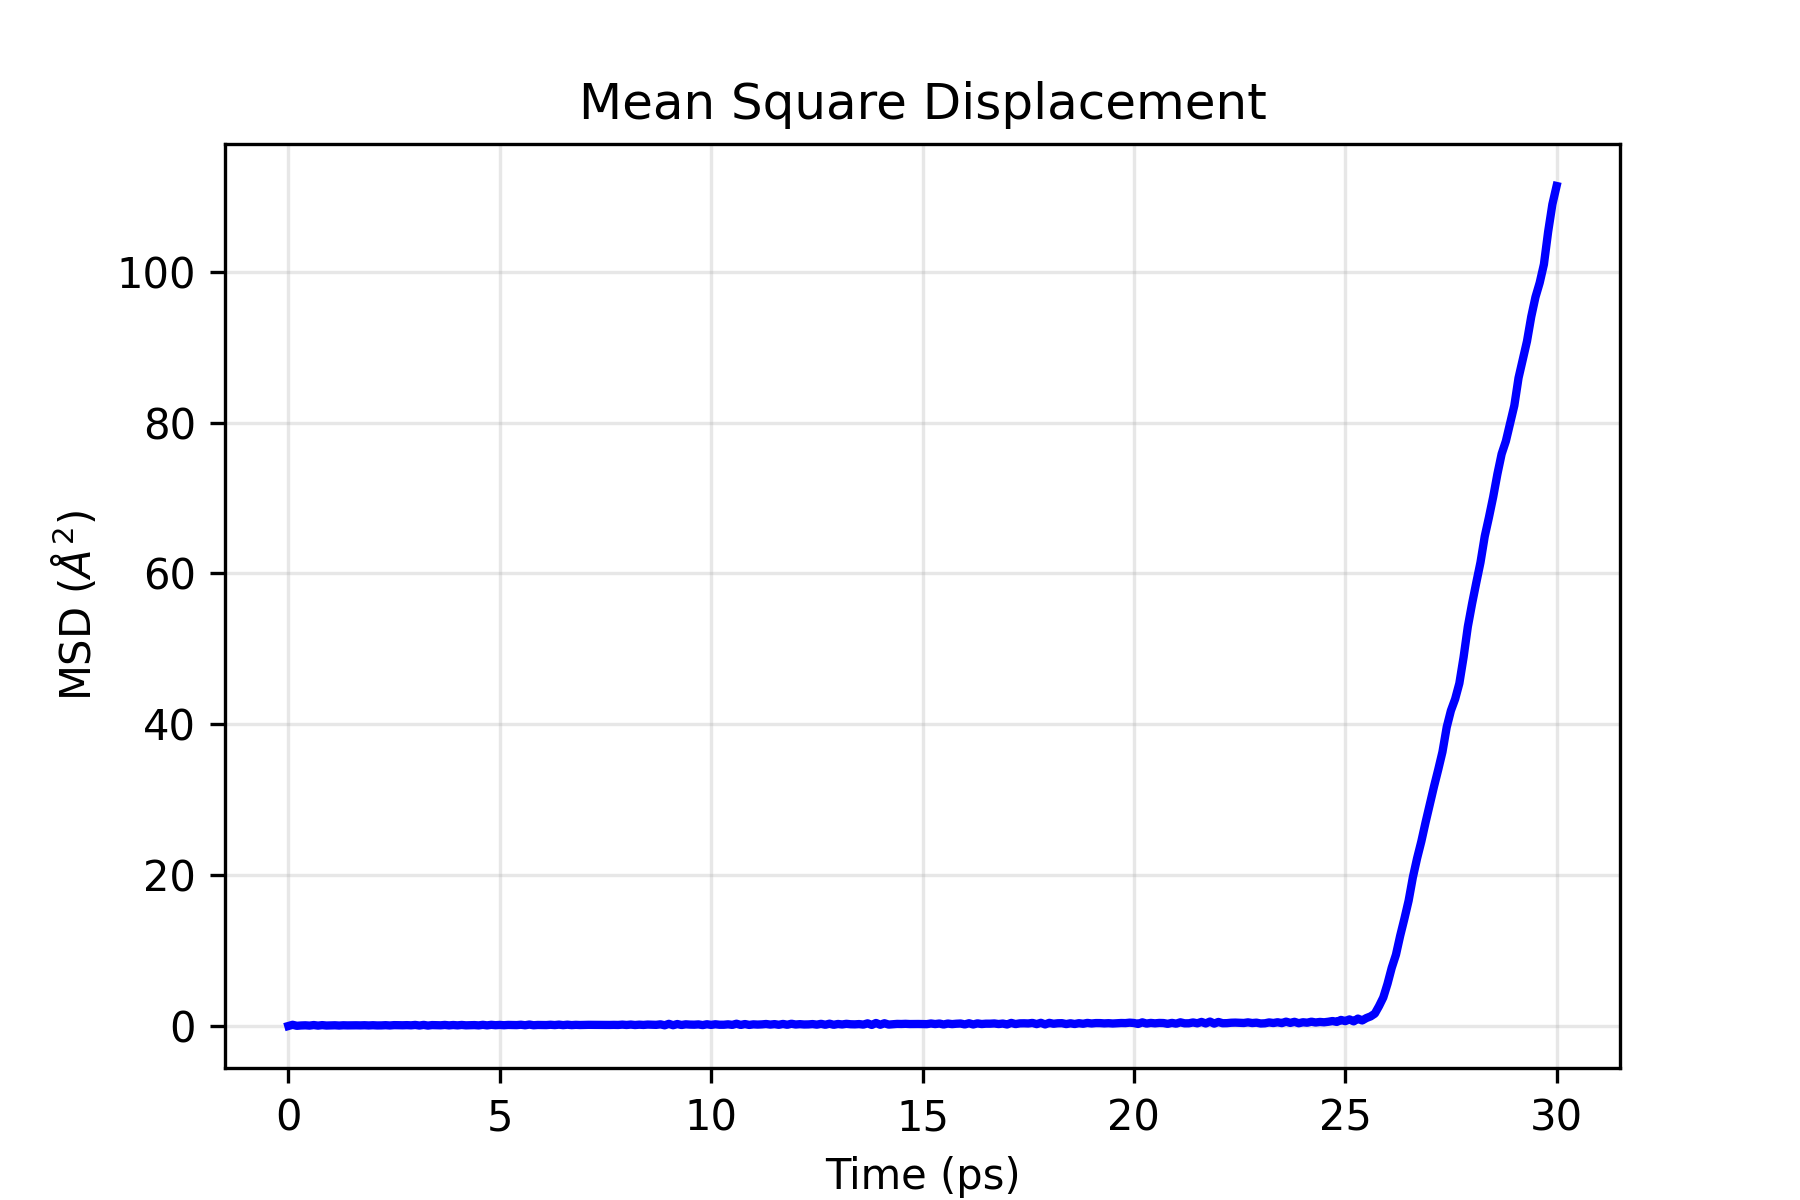
\includegraphics[width=\linewidth]{../python/msd/melt_P22_msd_output.png}
        \caption{Mean square displacement}
        \label{fig:sfig2}
    \end{subfigure}
    \\[1em]
    \begin{subfigure}{0.48\textwidth}
        \centering
        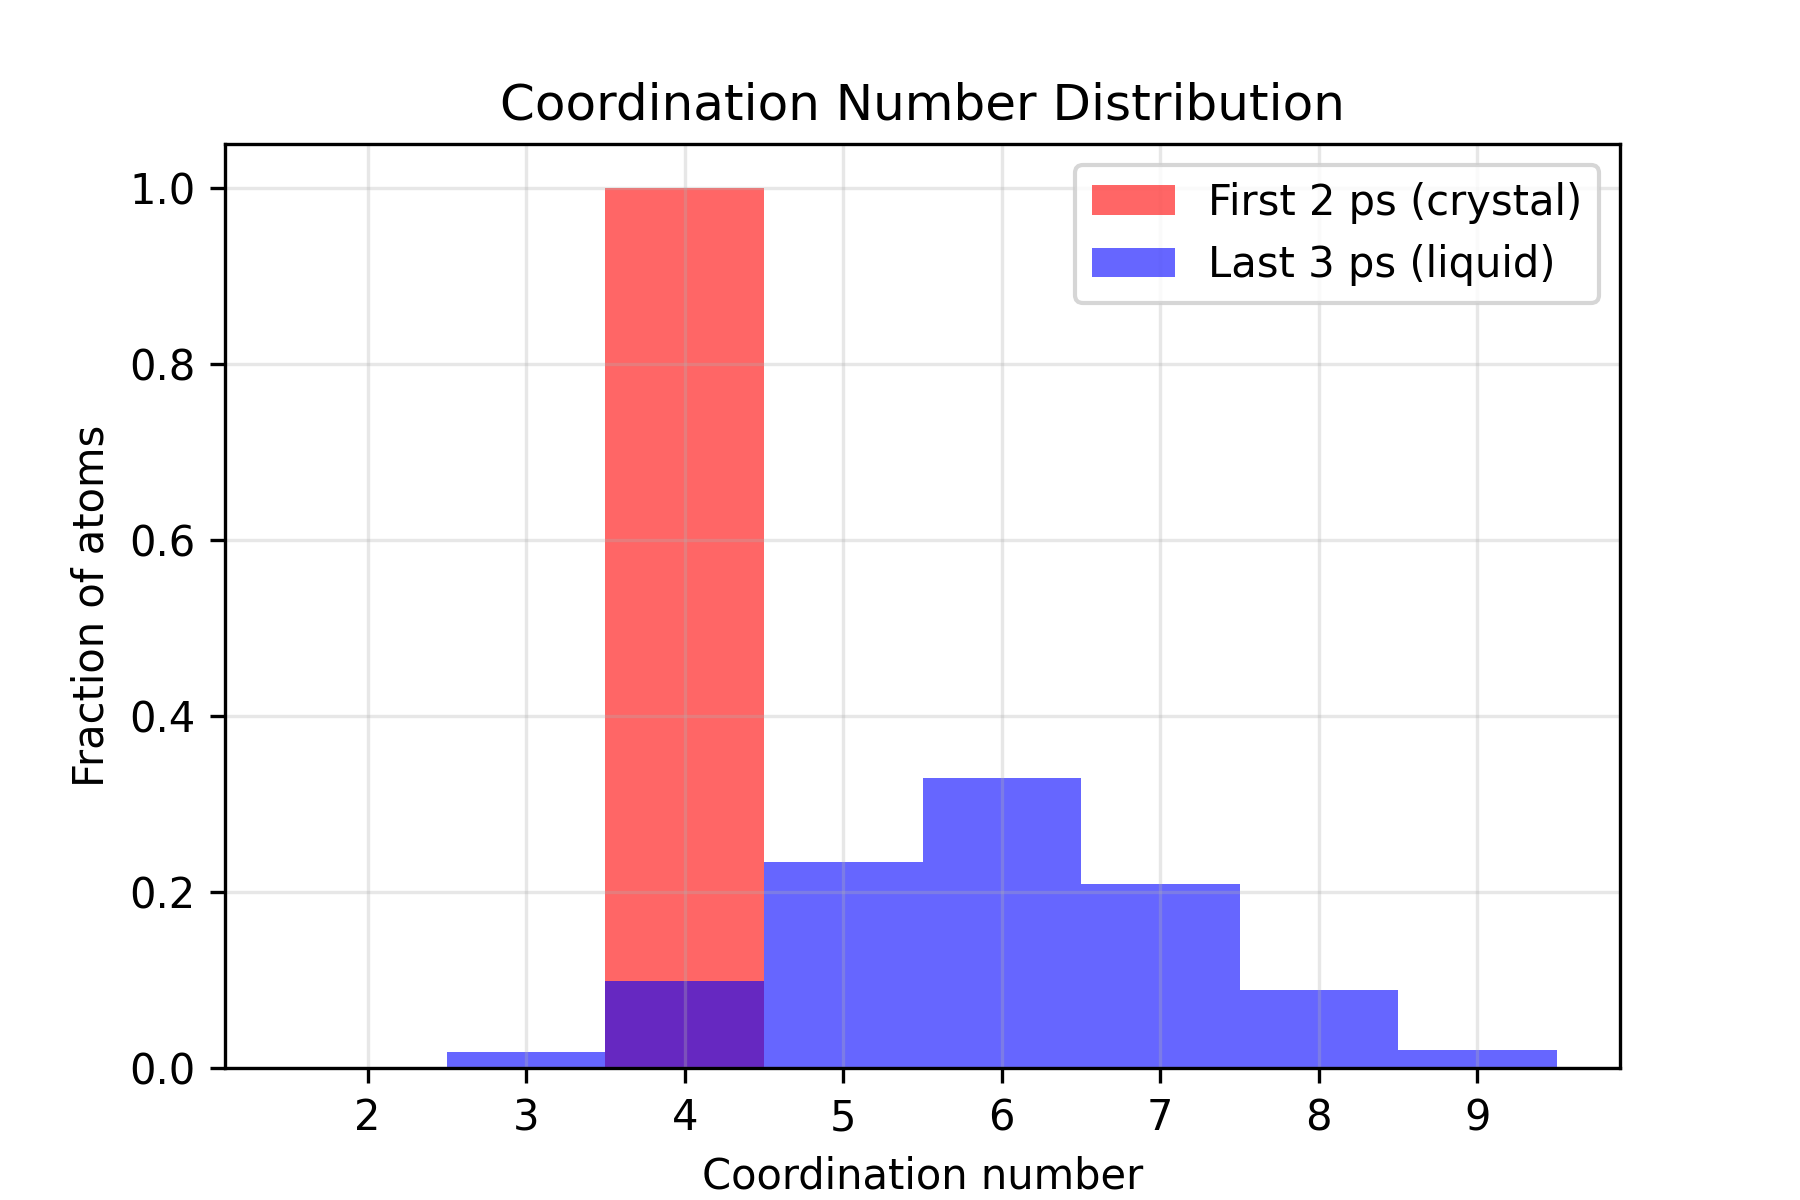
\includegraphics[width=\linewidth]{../python/coord_num/melt_P22_cn_output.png}
        \caption{Coordination number}
        \label{fig:sfig3}
    \end{subfigure}
    \hfill
    \begin{subfigure}{0.48\textwidth}
        \centering
        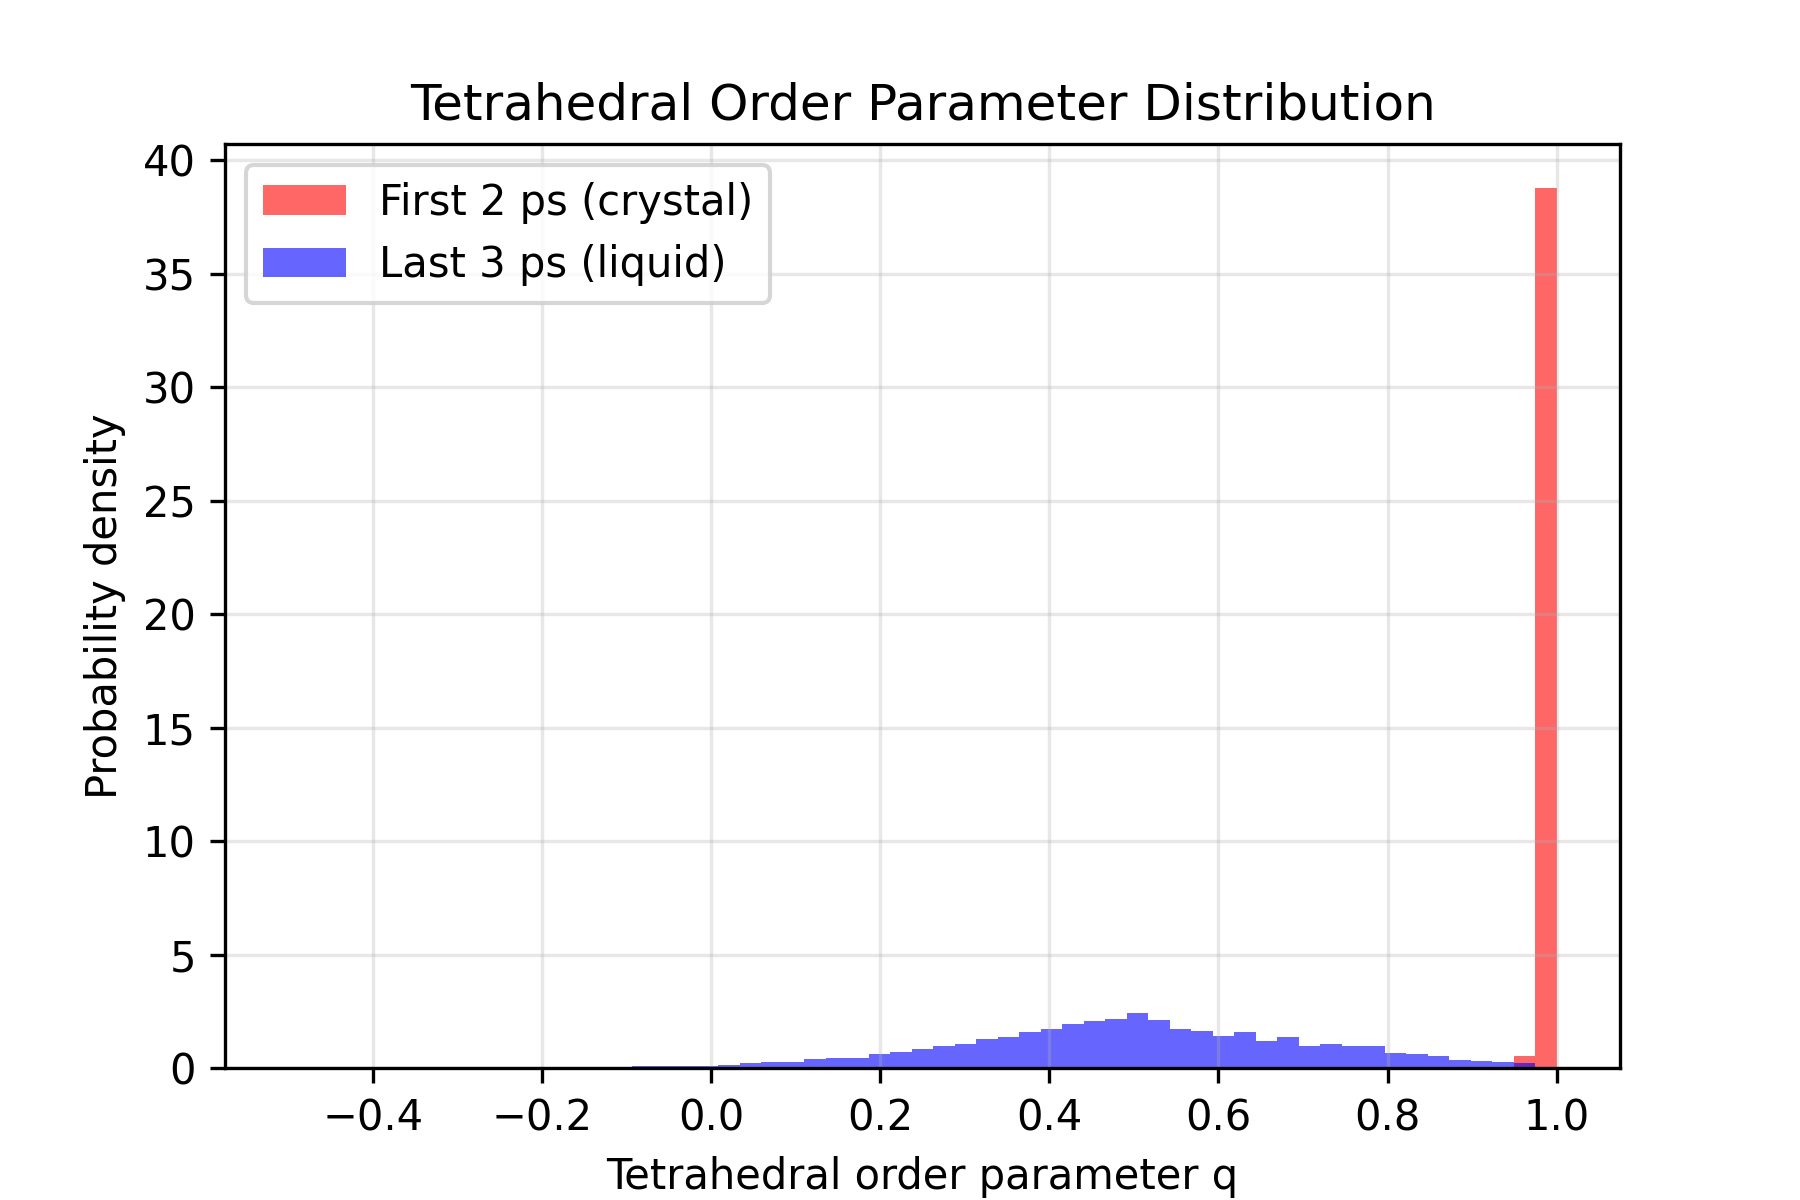
\includegraphics[width=\linewidth]{../python/top/melt_P22_top_output.png}
        \caption{Tetrahedral order parameter}
        \label{fig:sfig4}
    \end{subfigure}
    \caption{Structural and dynamical evidence for melting in the 216-atom system heated to 2500~K with \texttt{22.almtp}. Red curves and histograms are computed over the first 2~ps of the ramp, blue over the final 3~ps. (a) $g(r)$ collapses from sharp diamond-lattice shells persisting to 8~\AA{} into a single broad peak damping to unity by 3.5~\AA. (b) The MSD is bounded below $1$~\AA$^2$ until 25.5~ps, then grows linearly, confirming diffusion. (c) Coordination shifts from a delta function at fourfold to a broad distribution peaking at sixfold. (d) The tetrahedral order parameter falls from $0.9925$ to $0.4977$ and broadens by a factor of 35.}
    \label{fig:melt_signatures}
\end{figure}

Loading the trajectory into VMD showed the ordered diamond lattice visibly breaking apart into a disordered liquid over the course of the run.

\begin{figure}[H]
    \centering
    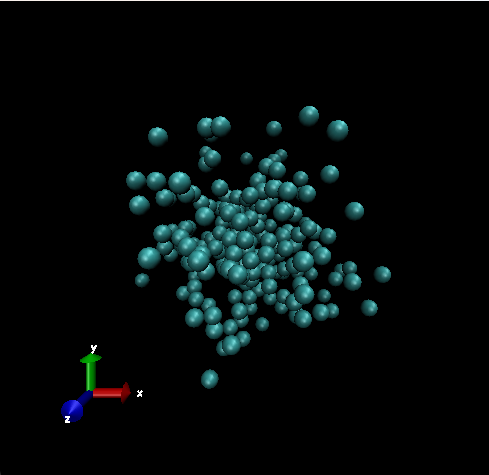
\includegraphics[width=0.5\textwidth]{melt_216_22almtp_2500K_final.png}
    \caption{Snapshot of the 216-atom system during the melt, visualized in VMD. The starting configuration is the ordered diamond lattice; over the 30~ps heating ramp to 2500~K it breaks down into a disordered liquid.}
    \label{fig:melt_vmd}
\end{figure}

\subsubsection{Hold P22}
\marginpar{July 28, 2026}
With a melted configuration in hand, the 1~ns hold at 2500~K was set up. Rather than rebuilding a lattice, this run continues directly from the melted state using \texttt{read\_data} on the saved configuration, with \texttt{fix npt} holding both the start and target temperature at 2500~K. Following the group's suggestion, the hold was run with the melt-stable potential and with all three pruned potentials for comparison.

The \texttt{22.almtp} hold ran to completion in 10~h 35~min on 8 cores. The temperature held around 2500~K throughout and the potential energy stayed stable near $-137{,}165$~eV with no drift, confirming the liquid is well behaved over the full nanosecond. Neighbour-list rebuilds numbered 30{,}215, as expected for a continuously diffusing liquid and in sharp contrast to the near-zero counts of the solid runs.

\subsubsection{Hold pruned\_1}
The same hold was repeated with \texttt{pruned\_1.almtp}. Crucially it did not become unstable: temperature and potential energy tracked the level-22 hold closely, with no blow-up despite the documentation's warning that pruned potentials may be unstable in melts. It finished $11.7\times$ faster.

\subsubsection{Hold pruned\_2}
The hold was also run with \texttt{pruned\_2.almtp}, the next level up in accuracy and cost. It too remained stable at 2500~K and sat between \texttt{pruned\_1} and the melt-stable potential in speed, $4.2\times$ faster than level 22, as expected from its intermediate cost.

\subsubsection{Melt P26}
The melt using \texttt{26.almtp} completed successfully, reaching 2500~K with the same signatures seen for \texttt{22.almtp}: violent pressure fluctuations and a jump in neighbour-list rebuilds (374 here against 400 for the level-22 melt). Level 26 was, however, markedly slower, consistent with its being the higher-level and more expensive potential. The same five structural and dynamical tests applied to the level-22 melt were repeated here:
 
\begin{itemize}
    \item \textbf{RDF.} Over the last 3~ps, a single broad peak at 2.44~\AA{} reaching $g(r) = 2.06$, with a shallow minimum of $0.90$ at 3.16~\AA{} and no structure beyond: $g(r)$ holds at unity out to the 8~\AA{} limit. The first 2~ps show the diamond lattice instead, with peaks at 2.37, 3.87 and 4.54~\AA{} persisting undamped to 8~\AA{} and minima falling to zero between shells.
    \item \textbf{Coordination number.} Counted within a 3.15~\AA{} cutoff, the first minimum of the liquid $g(r)$. The first 2~ps give exactly 4.000 neighbours per atom with 100\% fourfold coordination. The final 3~ps give a mean of 5.964, spread over 3- to 9-fold environments and peaking at sixfold (31.1\%).
    \item \textbf{Mean square displacement.} Bounded below $1$~\AA$^2$ for the first 25.6~ps, rising slowly from $0.09$ to $0.7$~\AA$^2$ as the thermal vibration amplitude grows with temperature. At 25.7~ps it turns sharply and grows linearly to $107.5$~\AA$^2$ by the end of the ramp.
    \item \textbf{Tetrahedral order parameter.} The first 2~ps give $q = 0.9923$ with a standard deviation of $0.0060$. The final 3~ps give $q = 0.4905$ with a spread of $0.2080$.
    \item \textbf{Density.} The box volume averages $4507$~\AA$^3$ over the solid portion of the ramp and $4326$~\AA$^3$ after the transition, giving
    \begin{equation*}
        \rho = \frac{216 \times 28.0855}{6.022 \times 10^{23} \times 4326 \times 10^{-24}} = 2.329~\text{g/cm}^3
    \end{equation*}
    against $2.235$~g/cm$^3$ for the solid, a contraction of $4.0\%$. This matches the $2.337$~g/cm$^3$ obtained with \texttt{22.almtp} to within $0.4\%$, and the contraction of $4.2\%$ seen there to within $0.2$ percentage points.
\end{itemize}
 
\begin{figure}[H]
    \centering
    \begin{subfigure}{0.48\textwidth}
        \centering
        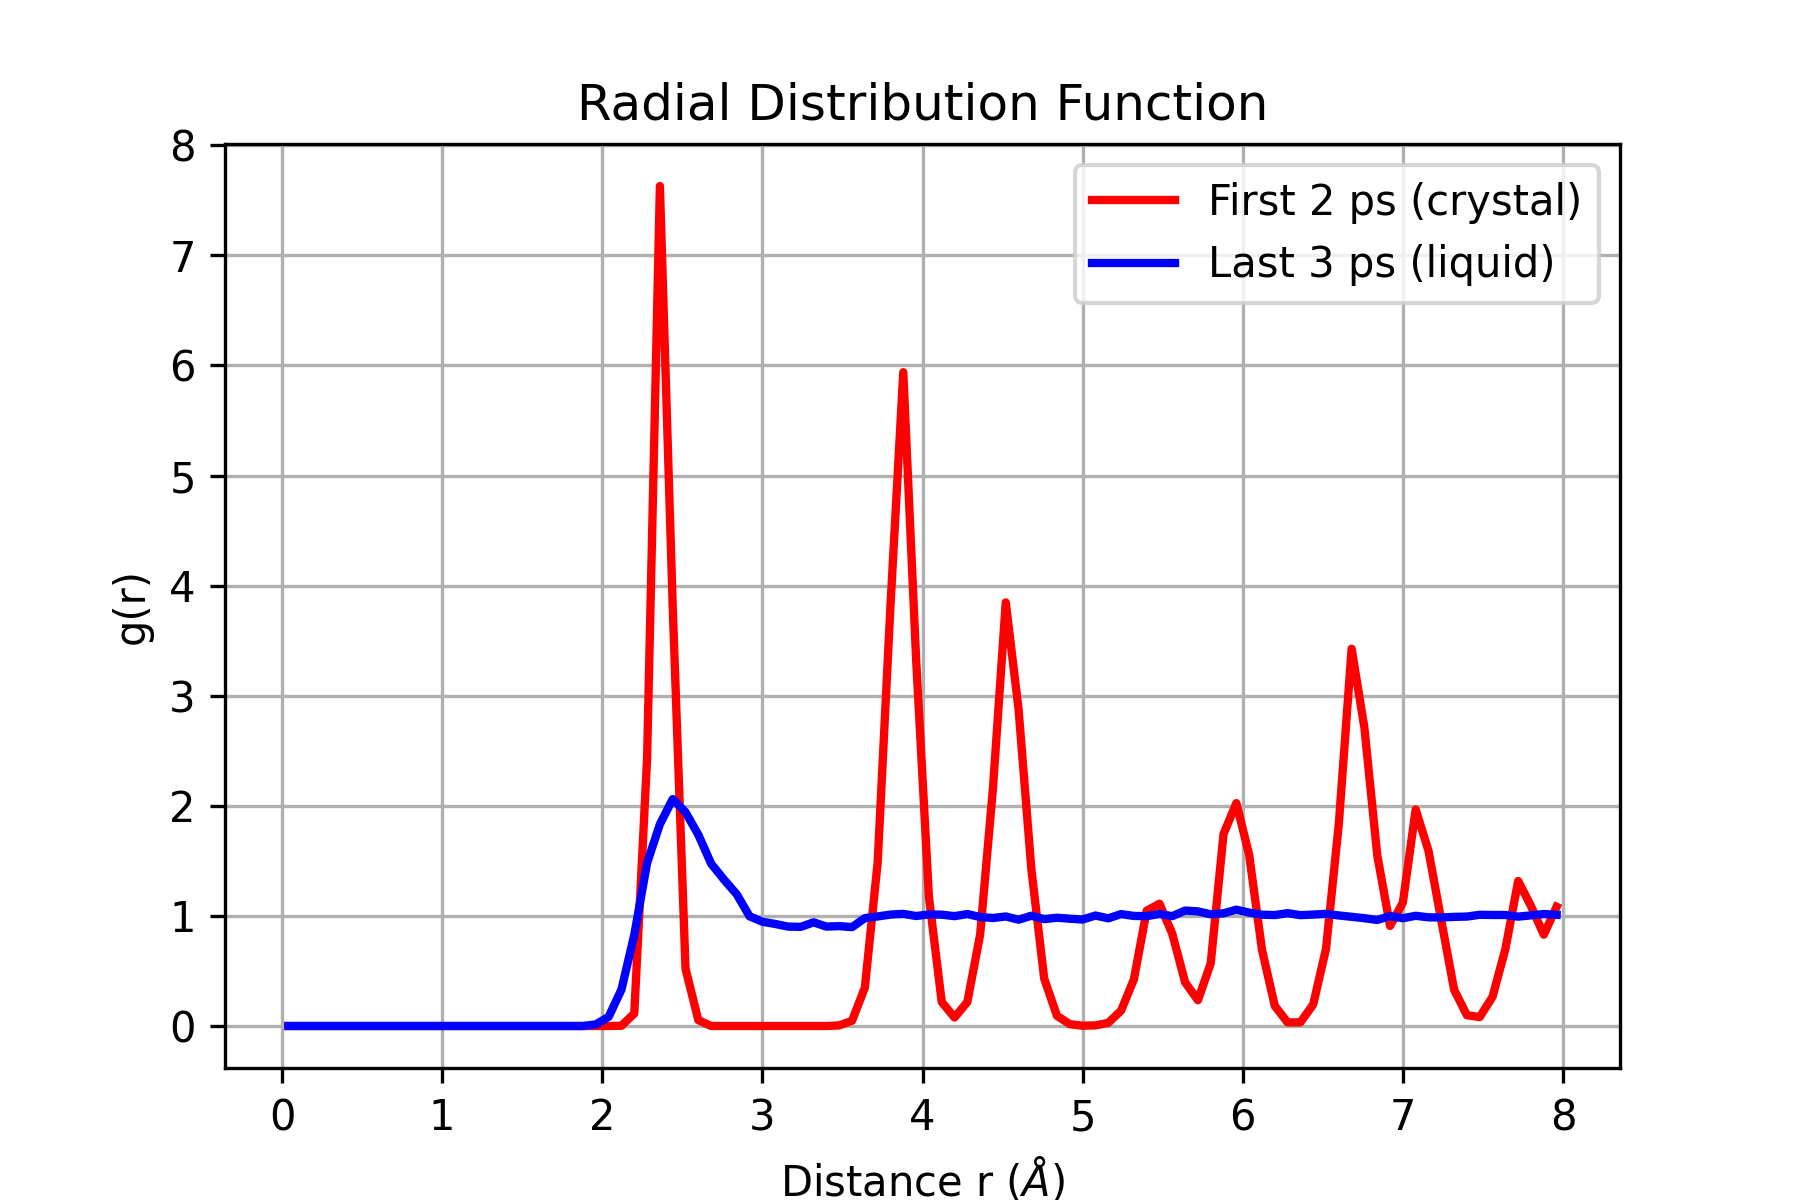
\includegraphics[width=\linewidth]{../python/radial_dist_fct/melt_P26_rdf_output.png}
        \caption{Radial distribution function}
        \label{fig:p26_rdf}
    \end{subfigure}
    \hfill
    \begin{subfigure}{0.48\textwidth}
        \centering
        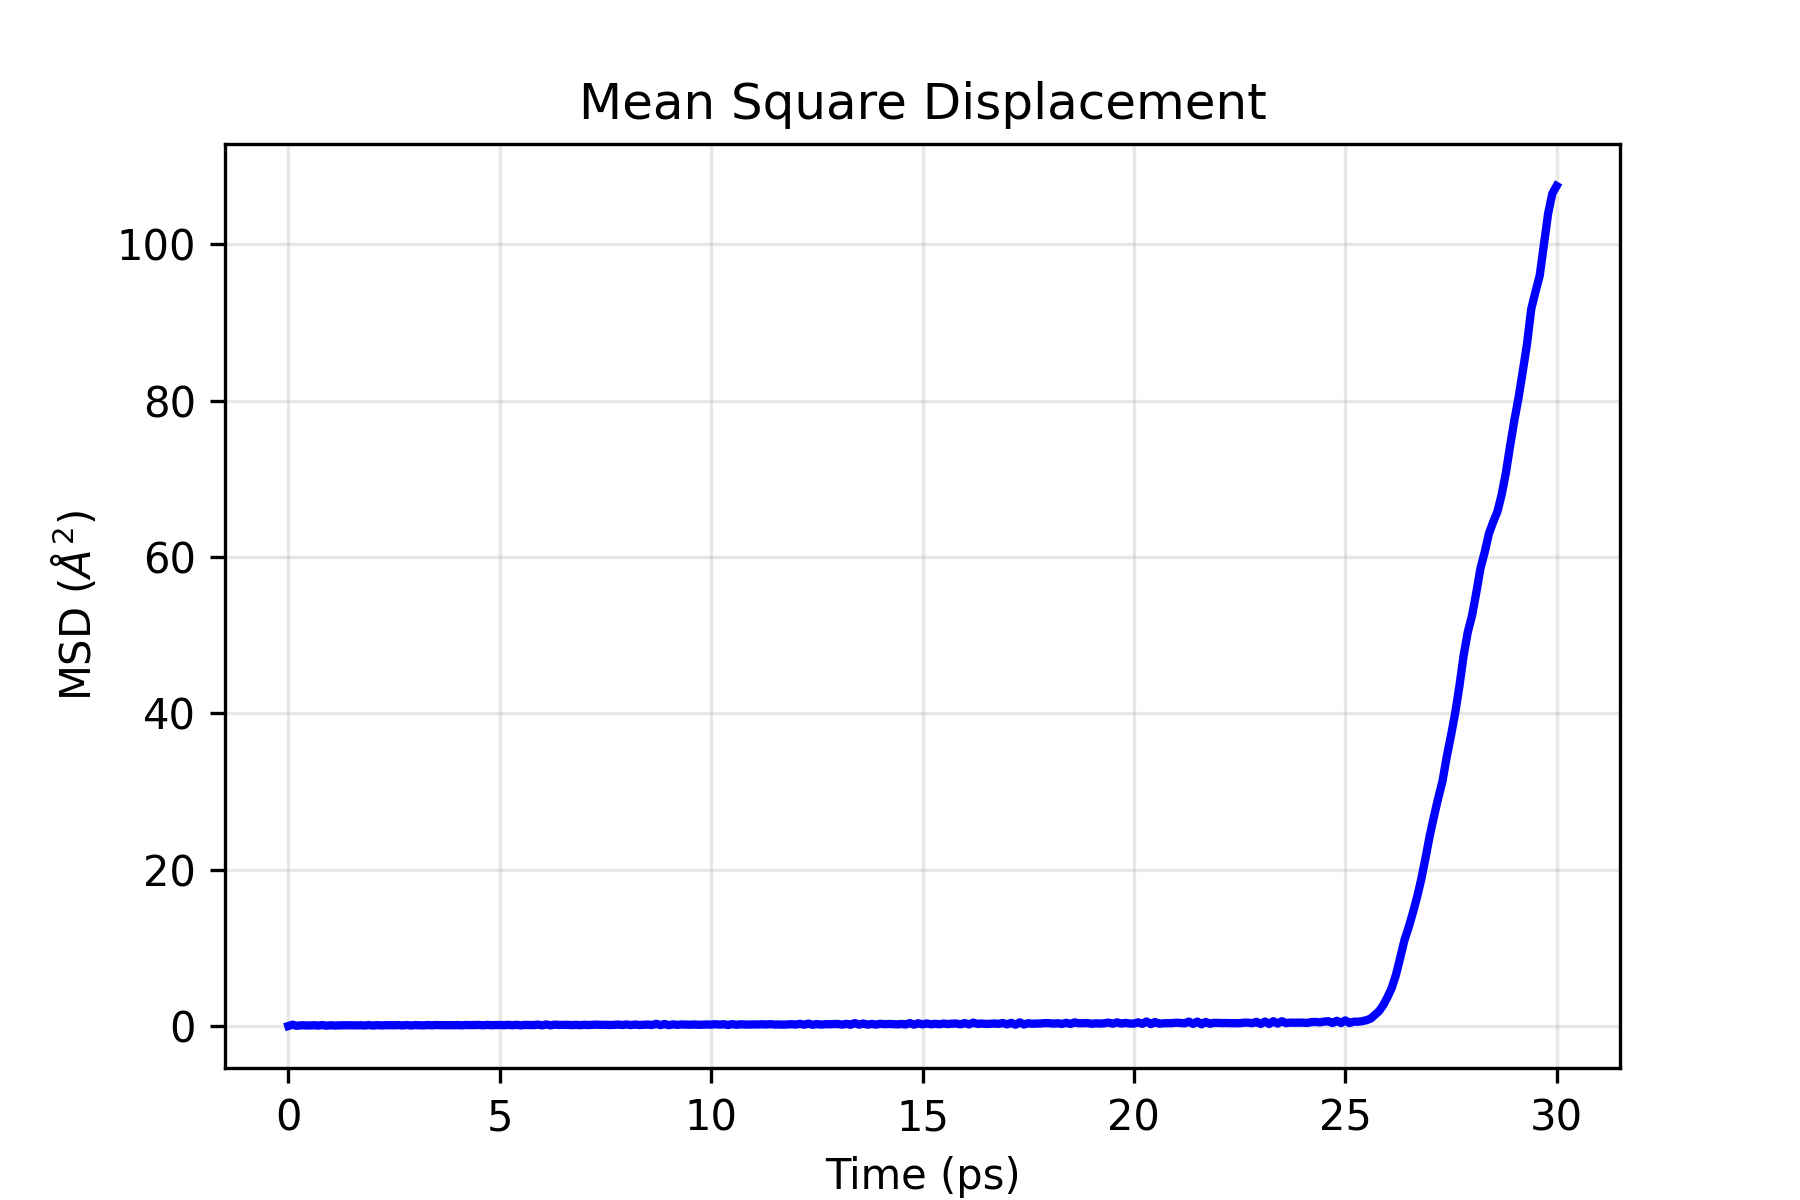
\includegraphics[width=\linewidth]{../python/msd/melt_P26_msd_output.png}
        \caption{Mean square displacement}
        \label{fig:p26_msd}
    \end{subfigure}
    \\[1em]
    \begin{subfigure}{0.48\textwidth}
        \centering
        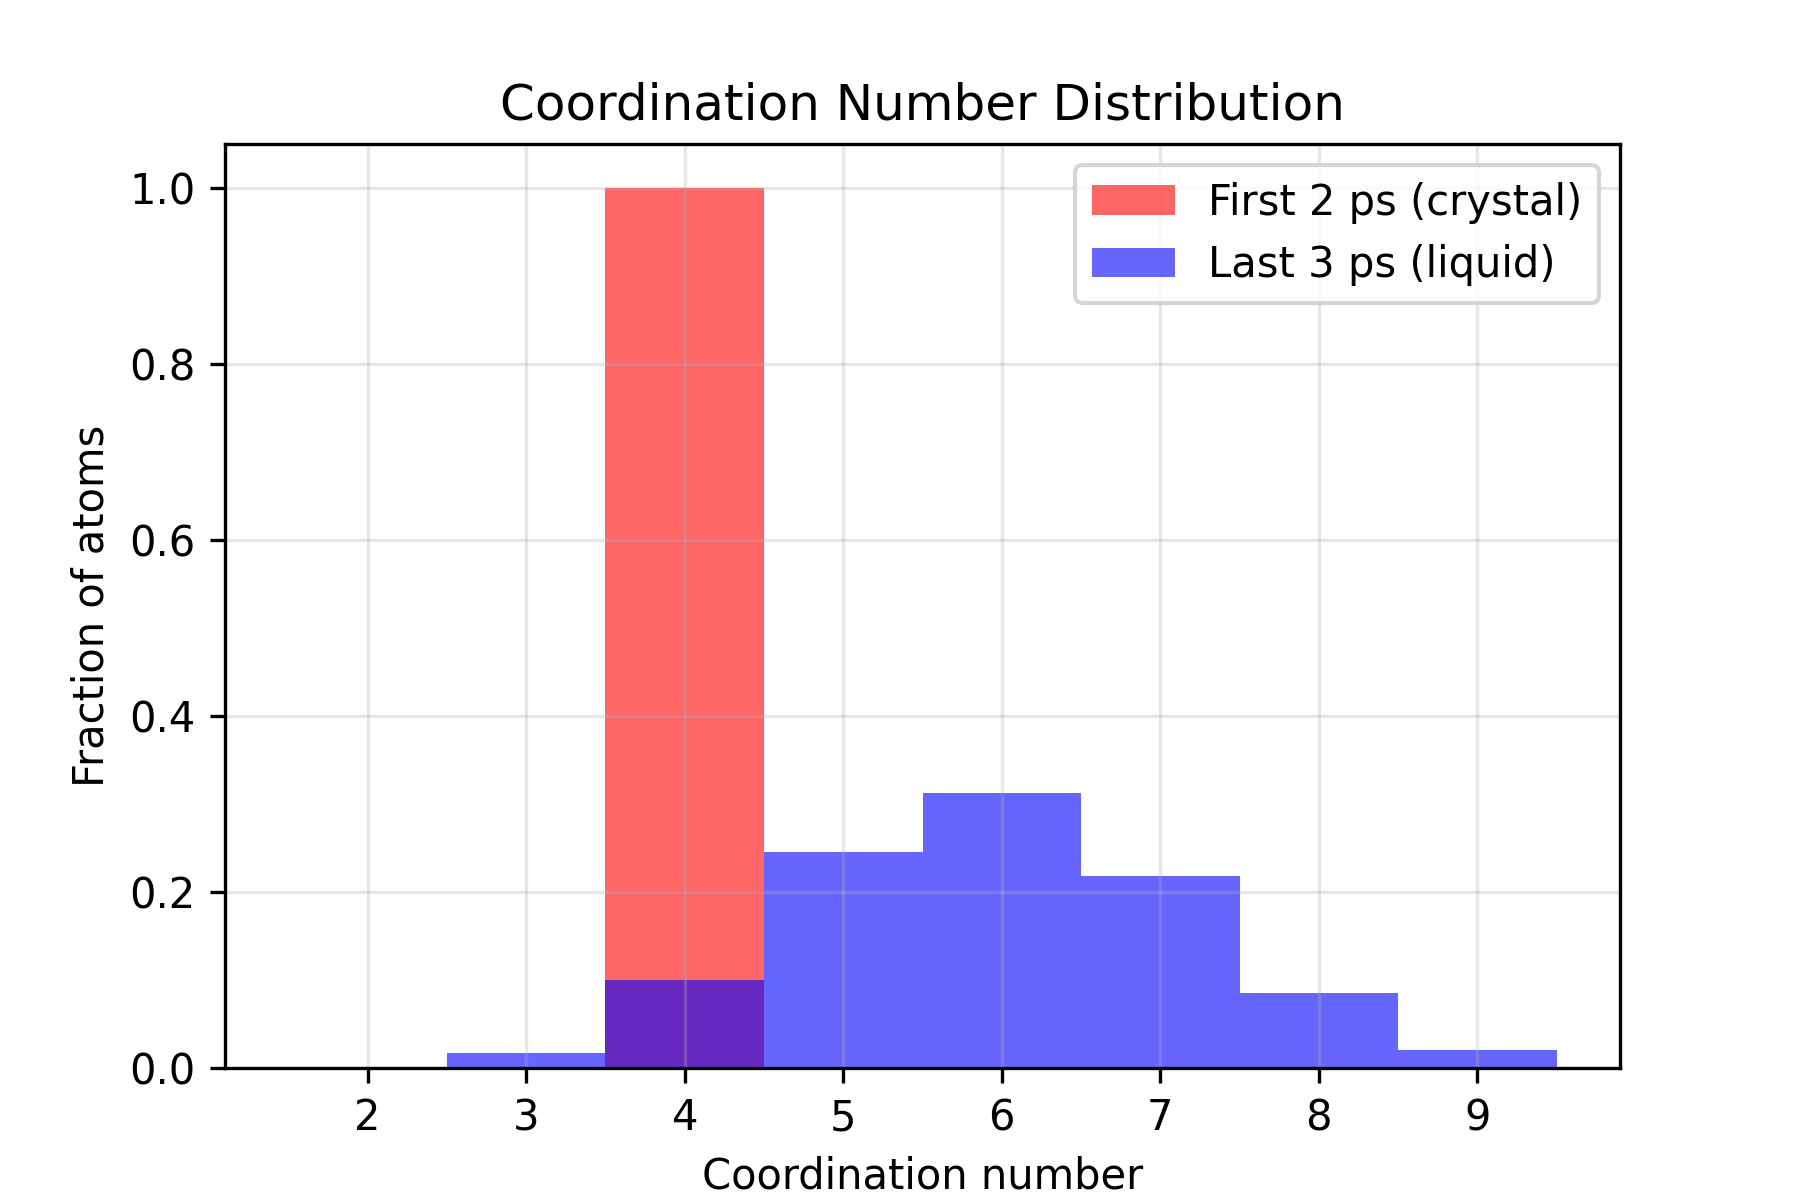
\includegraphics[width=\linewidth]{../python/coord_num/melt_P26_cn_output.png}
        \caption{Coordination number}
        \label{fig:p26_cn}
    \end{subfigure}
    \hfill
    \begin{subfigure}{0.48\textwidth}
        \centering
        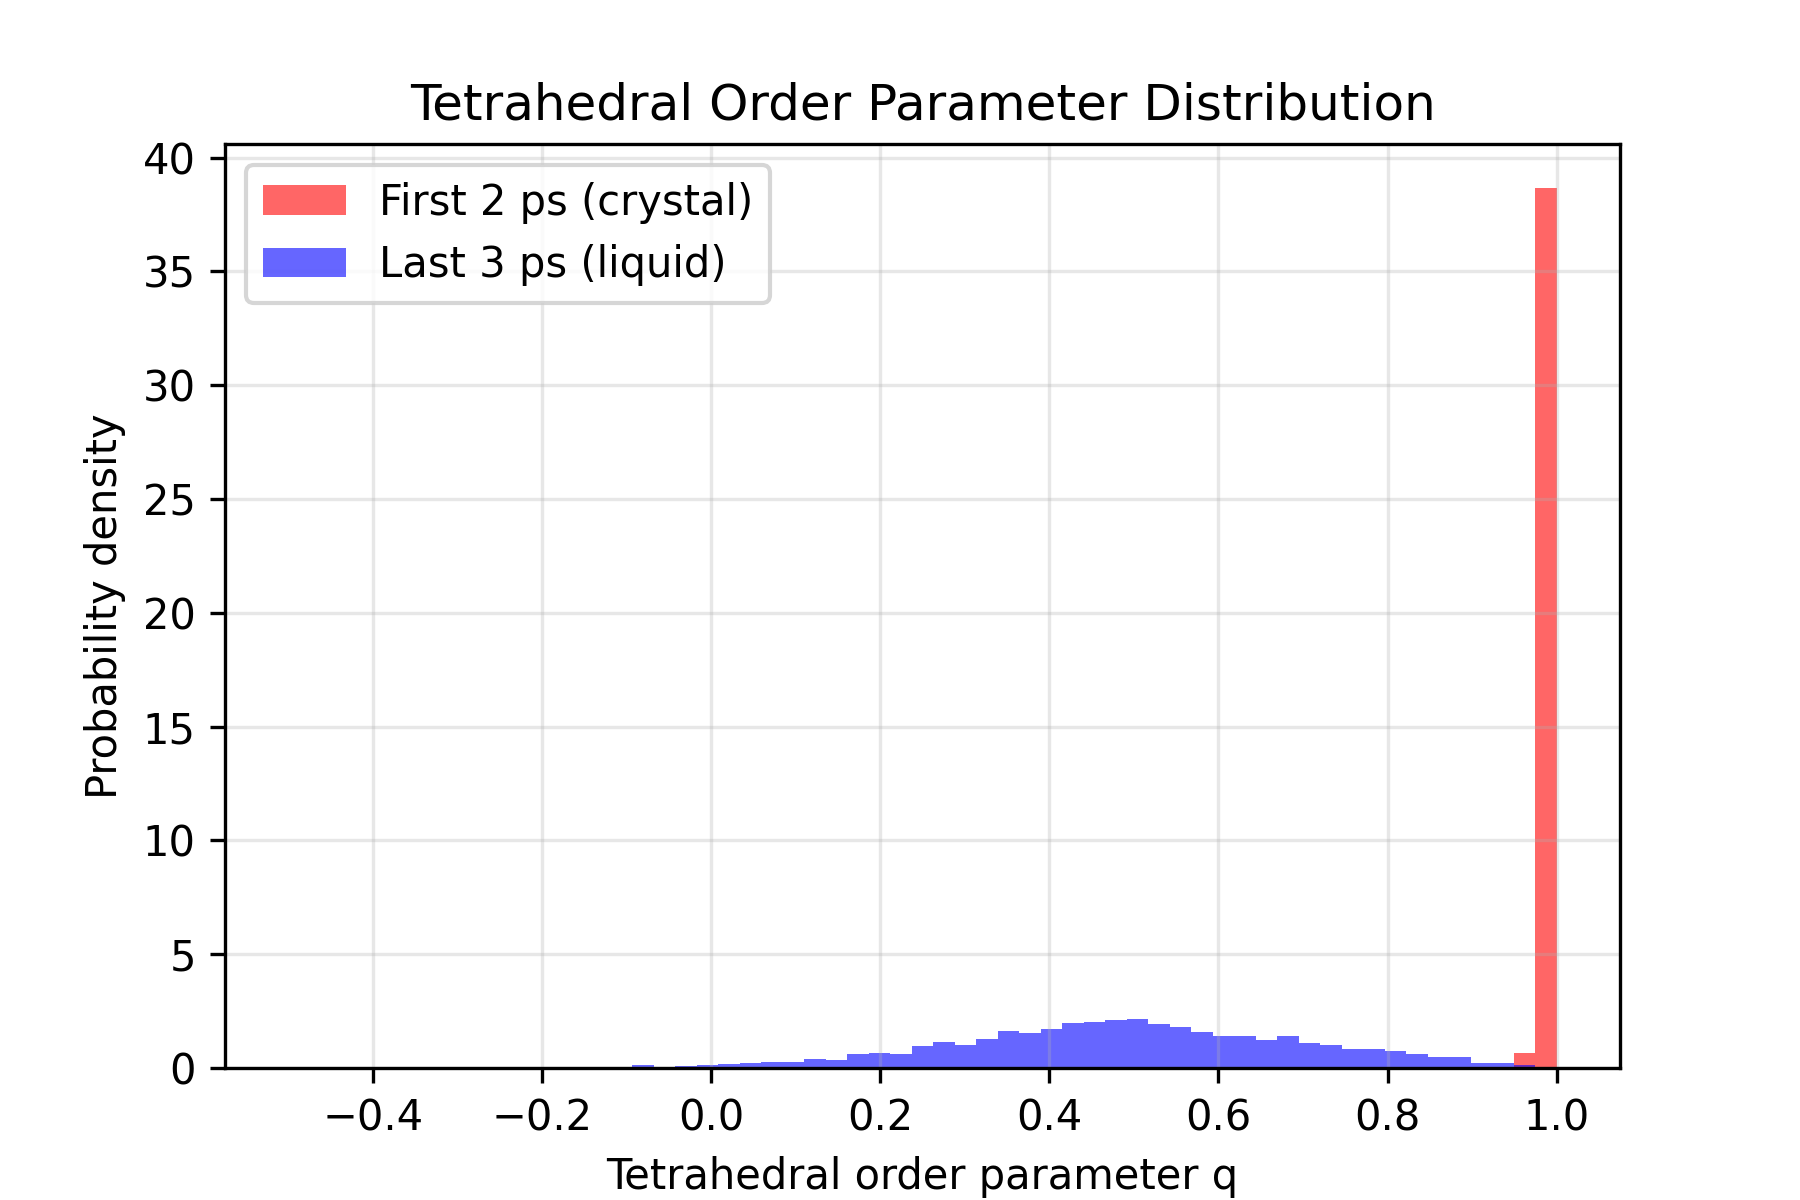
\includegraphics[width=\linewidth]{../python/top/melt_P26_top_output.png}
        \caption{Tetrahedral order parameter}
        \label{fig:p26_top}
    \end{subfigure}
    \caption{Structural and dynamical evidence for melting in the 216-atom system heated to 2500~K with \texttt{26.almtp}. Red curves and histograms are computed over the first 2~ps of the ramp, blue over the final 3~ps. (a) $g(r)$ collapses from sharp diamond-lattice shells persisting undamped to 8~\AA{} into a single broad peak at 2.44~\AA{} damping to unity by 3.5~\AA. (b) The MSD is bounded below $1$~\AA$^2$ until 25.6~ps, then grows linearly to $107.5$~\AA$^2$, confirming diffusion. (c) Coordination shifts from a delta function at fourfold to a broad distribution peaking at sixfold. (d) The tetrahedral order parameter falls from $0.9923$ to $0.4905$ and broadens by a factor of 35. Every quantity matches the level-22 melt of Fig.~\ref{fig:melt_signatures} to within $1.5\%$.}
    \label{fig:melt26_signatures}
\end{figure}
 
\paragraph{Comparison with the level-22 melt.}
The two melt-stable potentials produce the same liquid. The first peak of $g(r)$ falls at 2.44~\AA{} against 2.45~\AA, a difference of well under one histogram bin. The mean coordination number is 5.964 against 5.968, a difference of $0.07\%$. The melting transition begins at 25.7~ps against 25.6~ps, one dump frame apart. The density of the liquid is $2.329$ against $2.337$~g/cm$^3$ ($0.34\%$), obtained from a contraction on melting of $4.0\%$ against $4.2\%$. Neighbour-list rebuild counts, 374 against 400, are likewise indistinguishable. None of these differences is resolvable given the frame-to-frame scatter of a 216-atom cell.

One difference is reproducible rather than random. The tetrahedral order parameter of the level-26 liquid is lower than the level-22 value in both the melt ($0.4905$ against $0.4977$) and the hold ($0.4821$ against $0.4903$, Table~\ref{tab:hold_structural}), by $0.0072$ and $0.0082$ respectively. Two independent trajectories giving the same sign and essentially the same magnitude suggests a genuine systematic offset rather than scatter, but it amounts to under $2\%$ and is a factor of 25 below the standard deviation of the single-atom distribution in either run. It has no bearing on phase identification.

The cost difference is not marginal. Level 26 runs at 11.3~steps/s against 28.1 in the melt and 10.4 against 26.2 in the hold, a factor of $2.49$ and $2.53$. That the two ratios agree to $1.6\%$ across a temperature ramp and an isothermal run confirms the premium is a fixed per-force-evaluation cost rather than anything state-dependent. Since the two potentials return the same liquid, \texttt{22.almtp} is the correct choice for the melt and hold stages at 2500~K, and \texttt{26.almtp} was not carried into the quench.

\marginpar{July 29, 2026}
\subsubsection{Hold pruned\_3}
The final pruned variant, \texttt{pruned\_3.almtp}, also completed the full nanosecond without instability, in 6~h 31~min. Temperature held near 2500~K and the potential energy settled at $-137{,}161.5$~eV, matching the level-22 hold to within $0.002\%$. With 30{,}243 rebuilds and 94.47 neighbours per atom it is statistically indistinguishable from the reference trajectory in structure-agnostic terms. Its speedup over level 22 is only $1.6\times$, the smallest of the three pruned potentials, which is exactly what its position as the most expensive and most accurate pruned variant predicts. All three pruned potentials therefore survive a nanosecond in the liquid, and the cost ordering \texttt{pruned\_1} $<$ \texttt{pruned\_2} $<$ \texttt{pruned\_3} $<$ level 22 is reproduced cleanly by the timings.

\marginpar{July 30, 2026}
\subsubsection{Hold P26}
The hold was repeated with \texttt{26.almtp}, this time starting from the \texttt{26.almtp} melt so that melt and hold use the same potential. It was run for 400~ps rather than the full nanosecond; at 10.4~steps/s against 26.2 for level 22, a full nanosecond would have consumed the same wall time budget for no additional information. Indeed the two runs occupied almost identical wall time, 10:42:19 for 400{,}000 steps against 10:35:32 for $10^6$. It remained stable throughout, the potential energy settling at $-137{,}159.7$~eV against $-137{,}166.3$~eV for the level-22 hold (means over the last five printed steps), a difference of 0.03~eV/atom and well inside $k_BT = 0.22$~eV at 2500~K. The slowdown factor of $2.53$ tracks the melt ratio of $2.49$ almost exactly, so the level-26 premium is a fixed per-force-evaluation cost rather than anything state-dependent. Normalised to 1~ns it would take 26.8~h. Rebuilds (12{,}134) and neighbours per atom (93.6) are in line with every other run once scaled to the shorter trajectory.

\subsubsection{Benchmark Summary}

\begin{table}[H]
\centering
\small
\begin{tabular}{l|l|c|r|r|r|r}
\toprule
Run & Potential & Steps & Wall time & Steps/s & Rebuilds & Neighs/atom \\
\midrule
Melt (30~ps)  & \texttt{22.almtp}       & $3.0\times10^4$ & 0:17:47  & 28.1  & 400      & 91.0 \\
Melt (30~ps)  & \texttt{26.almtp}       & $3.0\times10^4$ & 0:44:13  & 11.3  & 374      & 92.5 \\
\midrule
Hold (1~ns)   & \texttt{22.almtp}       & $1.0\times10^6$ & 10:35:32 & 26.2  & 30{,}215 & 94.8 \\
Hold (0.4~ns) & \texttt{26.almtp}       & $4.0\times10^5$ & 10:42:19 & 10.4  & 12{,}134 & 93.6 \\
Hold (1~ns)   & \texttt{pruned\_1.almtp} & $1.0\times10^6$ & 0:54:24  & 307.2 & 30{,}200 & 91.2 \\
Hold (1~ns)   & \texttt{pruned\_2.almtp} & $1.0\times10^6$ & 2:30:32  & 110.7 & 30{,}164 & 94.8 \\
Hold (1~ns)   & \texttt{pruned\_3.almtp} & $1.0\times10^6$ & 6:31:03  & 42.6  & 30{,}243 & 94.5 \\
\bottomrule
\end{tabular}
\caption{Melt and hold runs for 216 atoms on 8 MPI tasks (1 OpenMP thread each, $\geq 98.7\%$ CPU use in every run). The \texttt{22.almtp} and pruned holds start from the \texttt{22.almtp} melted configuration; the \texttt{26.almtp} hold starts from the \texttt{26.almtp} melt and was run for 0.4~ns, so its throughput rather than its wall time is the comparable quantity. No run recorded any dangerous neighbour-list builds.}
\label{tab:melt_hold_bench}
\end{table}

Three points follow from Table~\ref{tab:melt_hold_bench}. First, the pruned potentials give a factor of $11.7$ (\texttt{pruned\_1}) and $4.2$ (\texttt{pruned\_2}) over the melt-stable potential at fixed system size and step count, with rebuild counts and average neighbour numbers essentially unchanged, so the speedup is a genuine reduction in force-evaluation cost and not an artefact of a differently behaved trajectory. Against \texttt{26.almtp} the same comparison gives $29.6$ and $10.7$. Second, the measured \texttt{22.almtp} hold cost of 10.6~h exceeds the 9.1~h projected in Table~\ref{tab:projected_cost} by about $16\%$, which is the penalty from the 30{,}215 neighbour-list rebuilds that the static 300~K benchmark did not incur, as anticipated. Third, the rebuild rate is invariant across all potentials at roughly $3.0\times10^{-2}$ rebuilds per step, as it must be, since it is set by the thermostat temperature and the neighbour skin rather than by the descriptor level.

\subsubsection{Structural Comparison of the Hold Trajectories}
\marginpar{August 3, 2026}

The benchmark timings of Table~\ref{tab:melt_hold_bench} establish that all five potentials complete a nanosecond in the liquid without instability, but they are structure-agnostic: matching wall times, rebuild counts and potential energies do not establish that the potentials produce the same liquid. This section applies the diagnostics of Section~\ref{sec:metrics} to the hold trajectories directly.

Unlike the melt, the hold is isothermal throughout, so there is no crystal-to-liquid contrast within a single run. The comparison is instead made across potentials, with \texttt{22.almtp} serving as the reference. All quantities are computed over the final 30~ps of each trajectory, by which point the liquid is fully equilibrated, using the same 3.15~\AA{} bond cutoff throughout.

\begin{table}[H]
\centering
\small
\begin{tabular}{l|c|c|c|c|c|c}
\toprule
Potential & $r_1$ (\AA) & $r_{\min}$ (\AA) & $\bar{n}$ & $q$ & $D$ ($10^{-8}$~m$^2$/s) & $\rho$ (g/cm$^3$) \\
\midrule
\texttt{22.almtp}        & 2.44 & 3.24 & 5.960 & 0.4903 & 3.70 & 2.32 \\
\texttt{26.almtp}        & 2.44 & 3.32 & 5.949 & 0.4821 & 5.26 & 2.31 \\
\texttt{pruned\_1.almtp} & 2.44 & 3.24 & 5.925 & 0.4966 & 4.79 & 2.30 \\
\texttt{pruned\_2.almtp} & 2.44 & 3.24 & 5.912 & 0.4975 & 4.08 & 2.29 \\
\texttt{pruned\_3.almtp} & 2.44 & 3.32 & 5.970 & 0.4852 & 4.46 & 2.31 \\
\bottomrule
\end{tabular}
\caption{Structural and dynamical properties of the liquid at 2500~K for each potential, computed over the final 30~ps of each hold. $r_1$ is the first peak of $g(r)$ and $r_{\min}$ the first minimum; the second peak is a shoulder of $g(r) \approx 1.02$ near 4~\AA{} and is too weak to locate reliably. $\bar{n}$ is the mean coordination number within a 3.15~\AA{} cutoff, $q$ the mean tetrahedral order parameter, $D$ the self-diffusion coefficient from the Einstein relation, and $\rho$ the density from the mean box volume. The \texttt{26.almtp} hold is 0.4~ns rather than 1~ns, so its dynamical statistics are correspondingly poorer.}
\label{tab:hold_structural}
\end{table}

\begin{figure}[H]
    \centering
    \begin{subfigure}{0.48\textwidth}
        \centering
        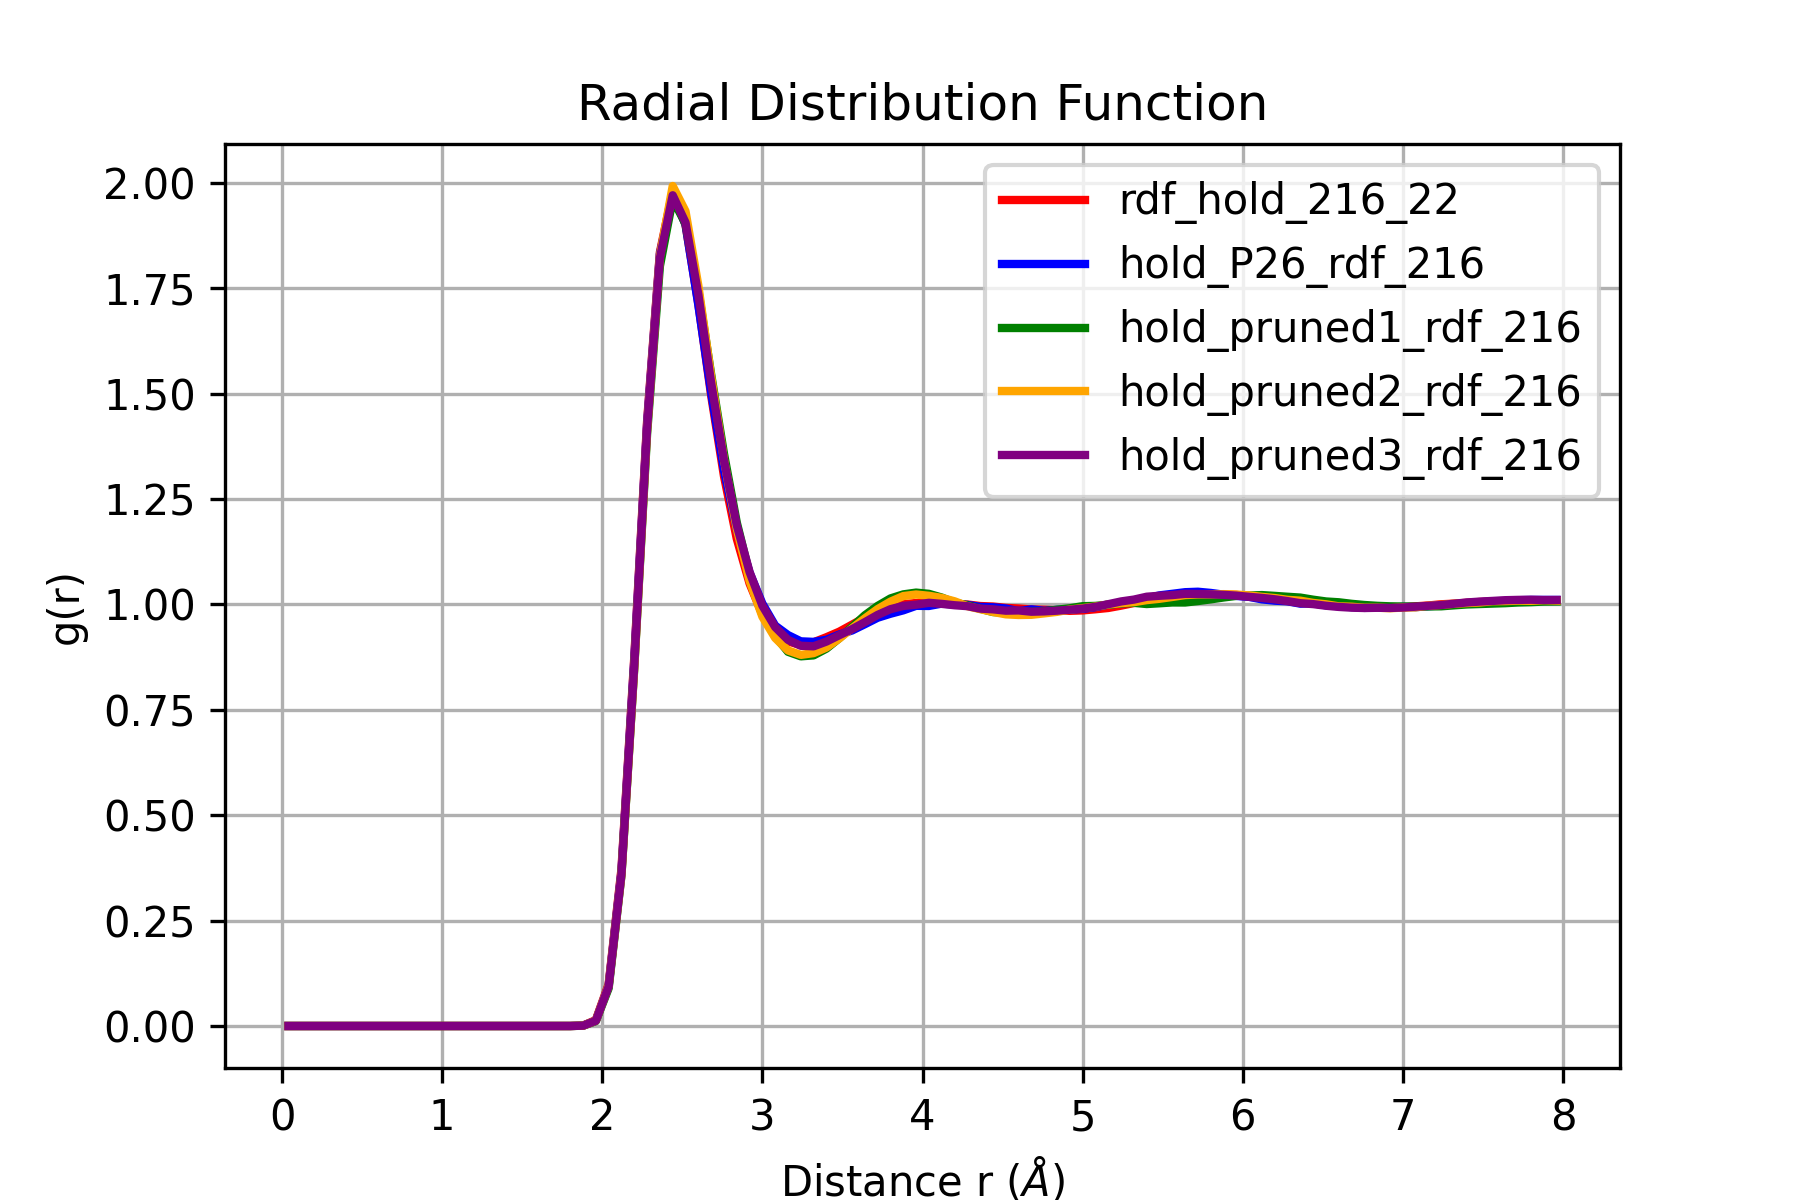
\includegraphics[width=\linewidth]{../python/radial_dist_fct/hold_all_rdf_output.png}
        \caption{Radial distribution function}
        \label{fig:hold_rdf}
    \end{subfigure}
    \hfill
    \begin{subfigure}{0.48\textwidth}
        \centering
        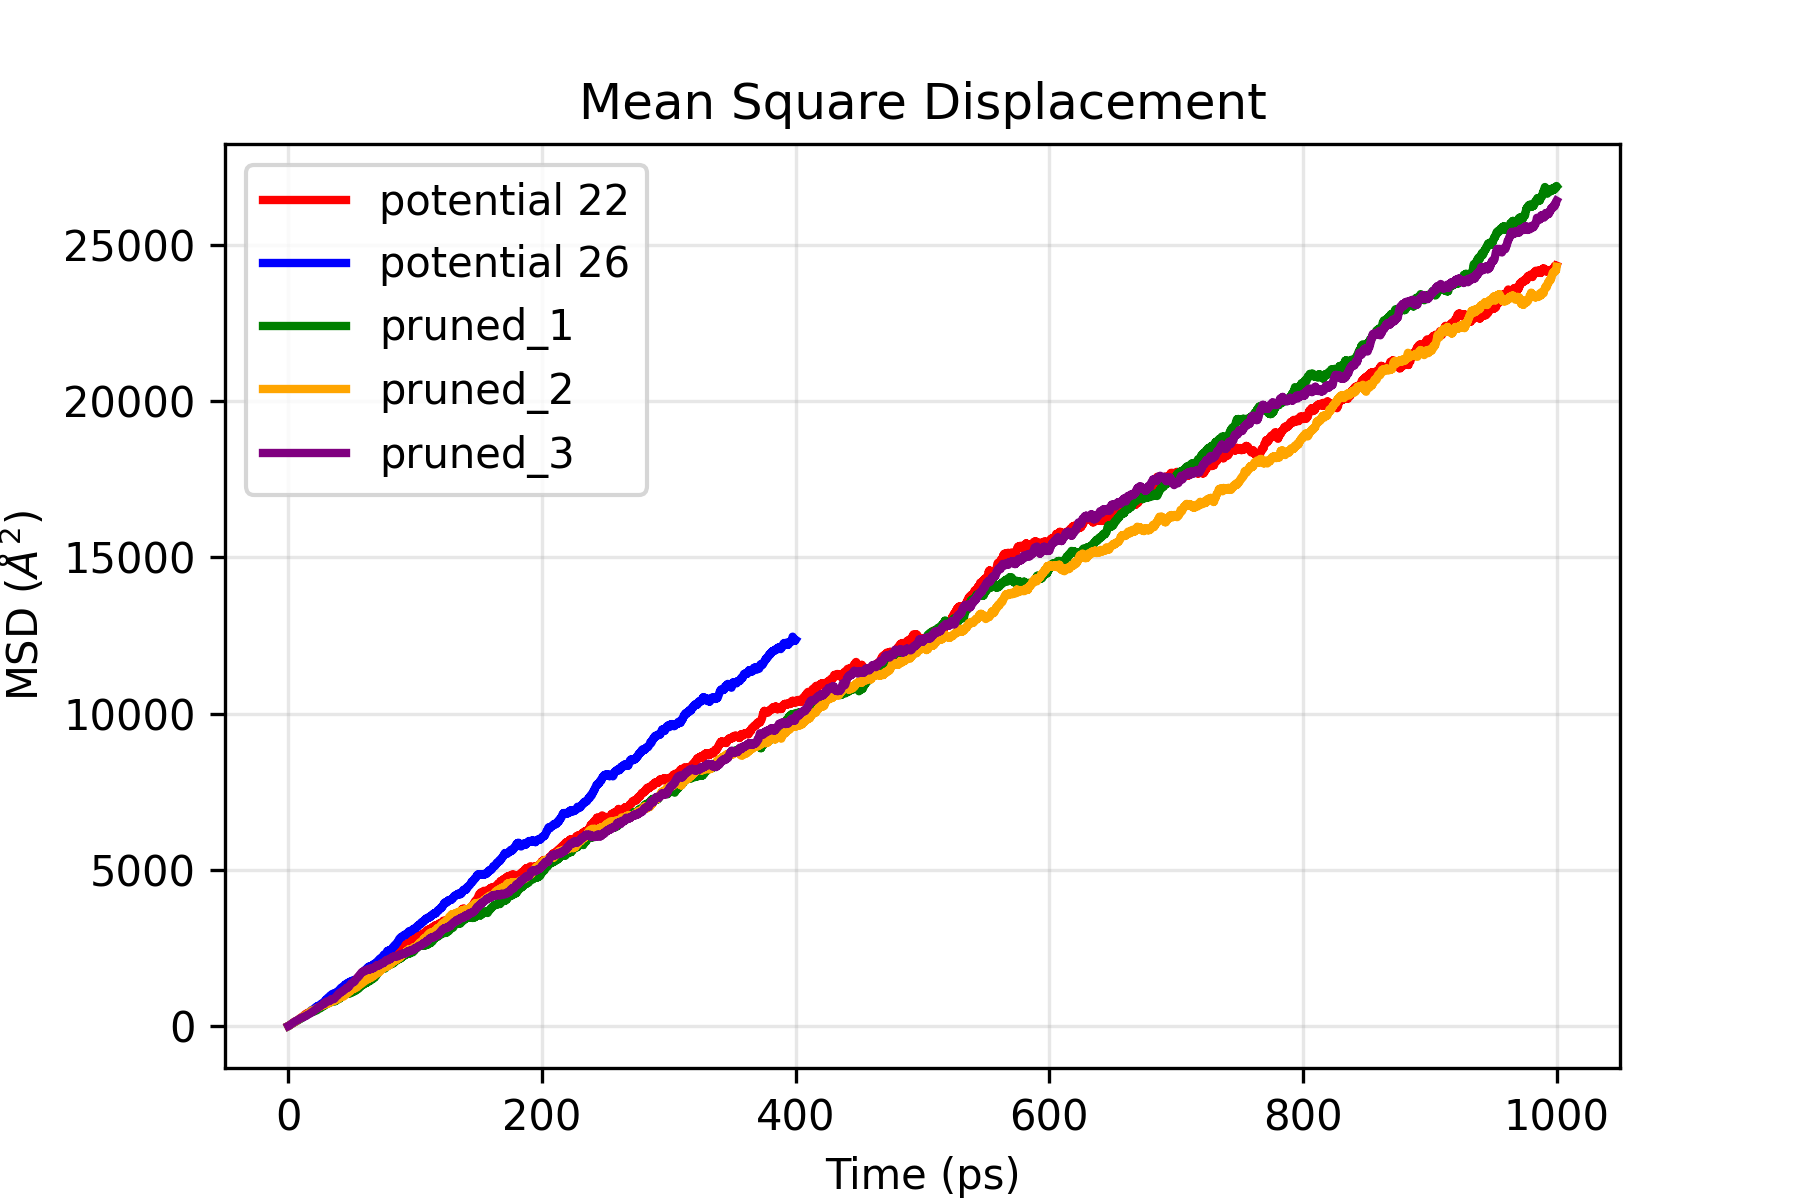
\includegraphics[width=\linewidth]{../python/msd/hold_all_msd_output.png}
        \caption{Mean square displacement}
        \label{fig:hold_msd}
    \end{subfigure}
    \\[1em]
    \begin{subfigure}{0.48\textwidth}
        \centering
        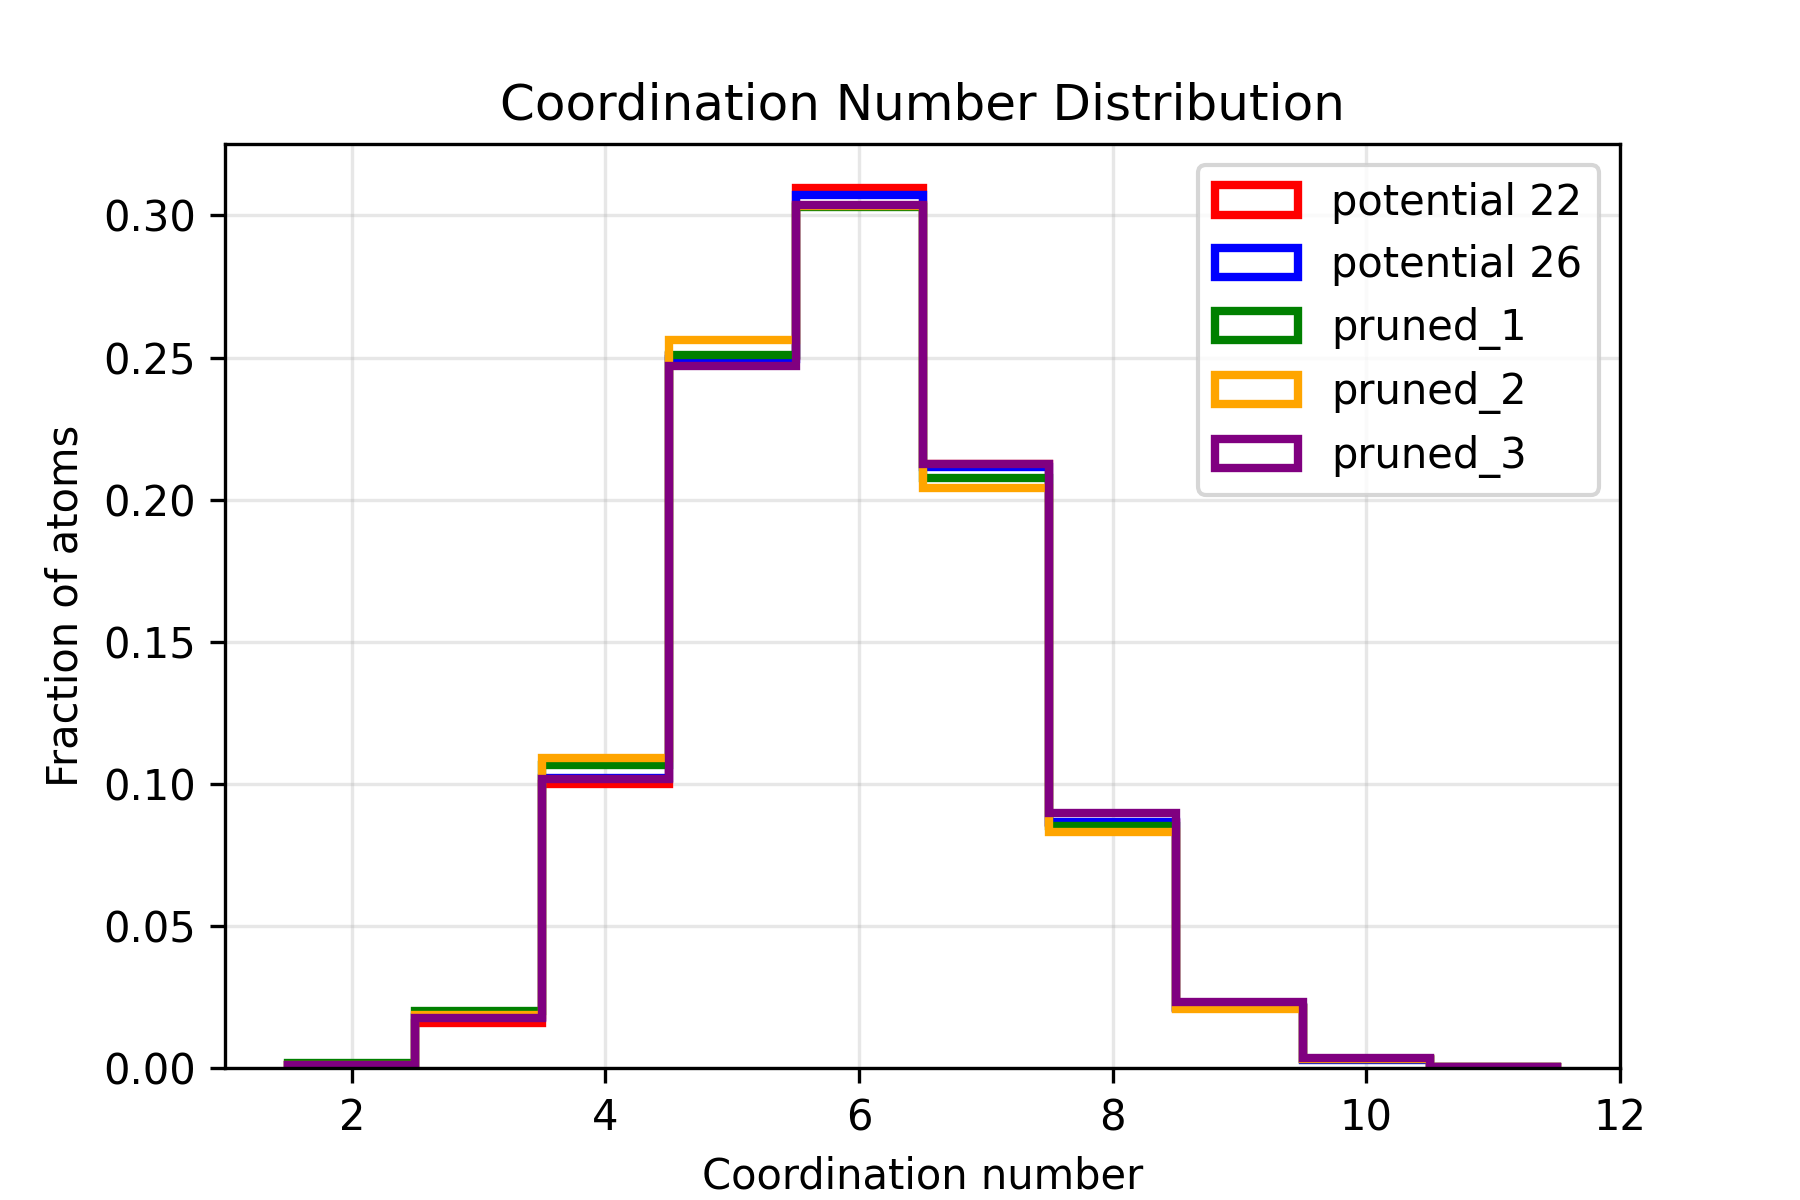
\includegraphics[width=\linewidth]{../python/coord_num/hold_all_cn_output.png}
        \caption{Coordination number}
        \label{fig:hold_cn}
    \end{subfigure}
    \hfill
    \begin{subfigure}{0.48\textwidth}
        \centering
        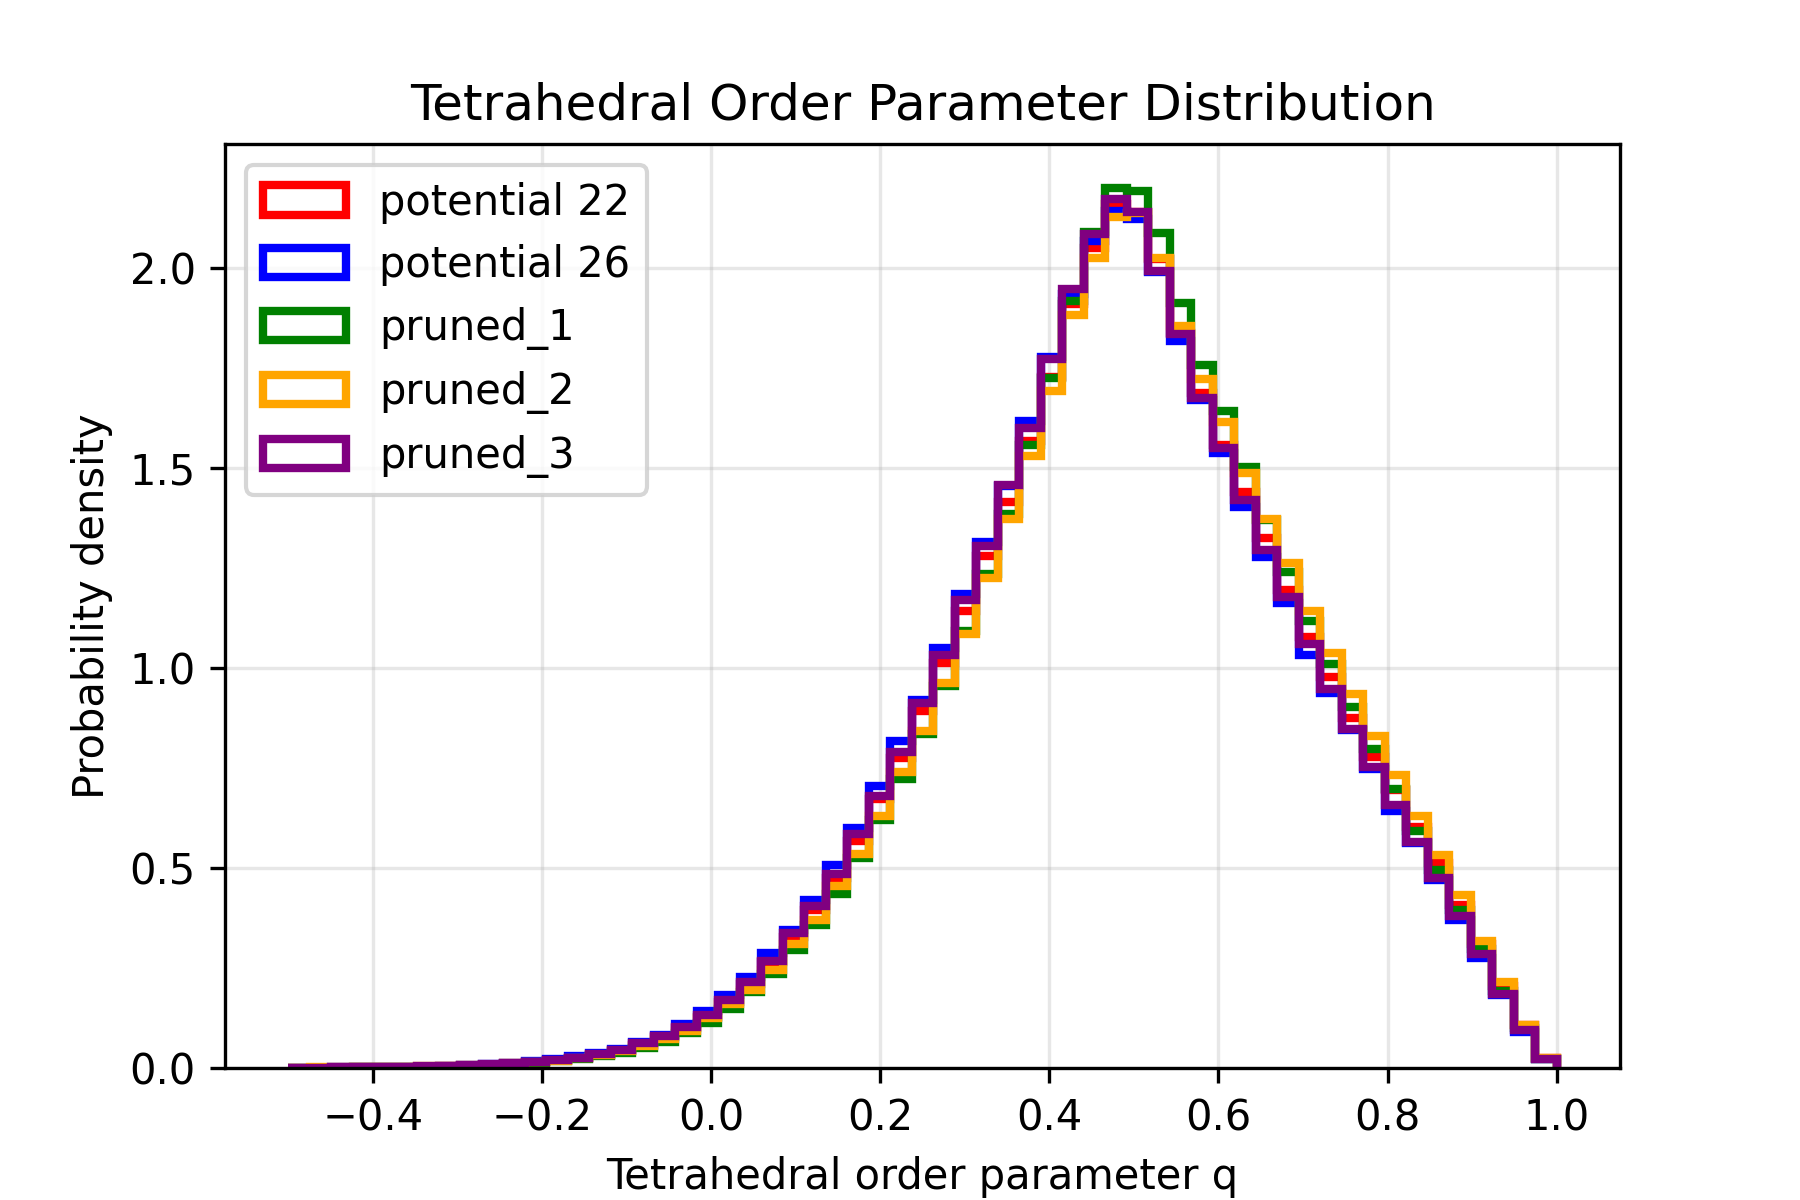
\includegraphics[width=\linewidth]{../python/top/hold_all_top_output.png}
        \caption{Tetrahedral order parameter}
        \label{fig:hold_top}
    \end{subfigure}
    \caption{All five hold trajectories at 2500~K, computed over the final 30~ps of each run. (a) The $g(r)$ curves are indistinguishable, sharing a first peak at 2.44~\AA{} and showing no structure beyond the first minimum. (b) The MSD is linear and unbounded for every potential, confirming a fully diffusive liquid; \texttt{26.almtp} is the only visible outlier and is also the only 0.4~ns run. (c) Coordination distributions overlay to within one percentage point at every coordination number. (d) The tetrahedral order parameter distributions are likewise indistinguishable, all peaking near $q = 0.5$.}
    \label{fig:hold_comparison}
\end{figure}

\paragraph{Do the pruned potentials reproduce the reference liquid?}
Yes, on every structural measure. The first peak of $g(r)$ falls at 2.44~\AA{} for all five potentials, the curves overlay to within the linewidth of Fig.~\ref{fig:hold_rdf}, and none shows structure beyond the first minimum. Mean coordination spans 5.912 to 5.970, a range of $1.0\%$, and the full distributions agree to within one percentage point at every coordination number. The tetrahedral order parameter spans 0.4821 to 0.4975, a range of $3.1\%$, with standard deviations identical to three decimal places.

Crucially the pruned potentials do not deviate systematically from the reference. \texttt{pruned\_3} gives the highest mean coordination of any potential, above both melt-stable ones, while \texttt{pruned\_2} gives the lowest; the ordering does not follow the pruning level. The small differences are therefore scatter rather than a monotonic degradation with descriptor reduction.

The dynamics are less tightly constrained. The self-diffusion coefficients span 3.70 to $5.26 \times 10^{-8}$~m$^2$/s, a spread of $42\%$, with \texttt{26.almtp} the outlier at the top. Two caveats apply. First, $D$ here is obtained from a single time origin rather than averaged over many, so its statistical uncertainty is far larger than that of the structural quantities. Second, the \texttt{26.almtp} hold is 0.4~ns against 1~ns for the others. The structural agreement is therefore the stronger result, and the diffusion spread should not be read as a physical difference between the potentials without a multiple-time-origin analysis.

\paragraph{Comparison with published liquid silicon.}
A direct comparison is limited by temperature. Zhao et al.~\cite{zhao2017} report the same tetrahedrality parameter for liquid silicon from \textit{ab initio} molecular dynamics, but their study concerns the metastable and supercooled liquid, spanning 1032 to 1800~K, whereas the present hold is at 2500~K, roughly 800~K above the melting point of 1687~K. Their $q_\text{tetra}$ falls between 0.52 and 0.68 over that range, increasing as the temperature is lowered. The value of $0.490 \pm 0.008$ obtained here sits just below their coldest-temperature values, which is the expected ordering: tetrahedral character is progressively lost as the liquid is superheated, so a strongly superheated liquid should return a lower $q$ than any point in their range. The agreement is therefore consistent in trend rather than quantitative, and no like-for-like comparison is available without repeating the hold nearer the melting point.

Zhao et al. report only $q_\text{tetra}$, the translational order parameter, the diffusion coefficient and the two-body excess entropy, so the first peak position and coordination number of the present liquid have no counterpart in that work.

\paragraph{Implication for the quench.}
The pruned potentials reproduce the reference liquid to within a few percent on every structural measure, so the hand-off in the melt-quench protocol is structurally justified: a configuration passed from the melt-stable potential to a pruned one at the start of the quench is not distinguishable from one the pruned potential would have generated itself. Combined with the $11.7\times$ speedup of \texttt{pruned\_1} in Table~\ref{tab:melt_hold_bench}, the cost saving is available at no measurable structural penalty in the liquid phase.

Whether the agreement survives the quench is a separate question. The potentials were shown in Section~\ref{sec:firstruns} to prefer different volumes in the solid, with \texttt{pruned\_1} holding a pressure of about $-12{,}400$~bar in a box where \texttt{22.almtp} sat at zero, so a divergence on cooling would not be surprising.


\subsection{Quench}
\marginpar{August 3, 2026}

Each liquid was cooled from 2500~K to 300~K at 1~K/ps under NPT at 0~bar ($2.2\times10^{6}$ steps at 1~fs), followed by a $1.5\times10^{5}$-step isothermal equilibration at 300~K. Each potential quenched its own hold configuration, so melt, hold and quench share a single force model within each run and the hand-off is not exercised here.

\begin{table}[H]
\centering
\small
\begin{tabular}{l|r|r|r|r}
\toprule
Potential & Total wall & 300~K block (steps/s) & Rebuilds & Neighs/atom \\
\midrule
\texttt{22.almtp}        & 24:34:31 & 29.2  & 73 & 93.31 \\
\texttt{pruned\_1.almtp} & 2:50:46  & 313.5 & 62 & 94.22 \\
\texttt{pruned\_2.almtp} & 6:31:05  & 106.9 & 18 & 92.56 \\
\texttt{pruned\_3.almtp} & \multicolumn{4}{c}{failed at step $2.94\times10^{5}$, see Section~\ref{sec:quench_fail}} \\
\bottomrule
\end{tabular}
\caption{Quench runs for 216 atoms on 8 MPI tasks. Rebuilds and neighbour counts are for the 300~K block only, since LAMMPS reports a single timing summary per \texttt{run} command. No dangerous builds in any run.}
\label{tab:quench_bench}
\end{table}

\begin{table}[H]
\centering
\small
\begin{tabular}{l|r|r|r|r}
\toprule
Potential & $T$ (K) & $E_{\text{pot}}$ (eV) & $V$ (\AA$^3$) & $\rho$ (g/cm$^3$) \\
\midrule
\texttt{22.almtp}        & 315.8 & $-137{,}279.75$ & 4482.4 & 2.247 \\
\texttt{pruned\_1.almtp} & 292.0 & $-137{,}276.65$ & 4397.9 & 2.291 \\
\texttt{pruned\_2.almtp} & 316.8 & $-137{,}279.86$ & 4477.9 & 2.250 \\
\bottomrule
\end{tabular}
\caption{Quenched state, averaged over the last five printed steps of the 300~K equilibration. The scatter in $T$ matches the $\pm17$~K expected from $\sqrt{2/3N}$ at $N=216$.}
\label{tab:quench_final}
\end{table}

Speedups fall relative to the liquid: \texttt{pruned\_1} gives $10.7\times$ and \texttt{pruned\_2} $3.7\times$ over \texttt{22.almtp}, against $11.7\times$ and $4.2\times$ in the hold. Pair time is $91.5\%$ of the loop for \texttt{22.almtp} but only $81.2\%$ for \texttt{pruned\_1}, with communication rising from $8.4\%$ to $13.2\%$; at 27 atoms per core the non-pair costs are close to fixed and cap the attainable speedup at $5.3\times$ regardless of descriptor level.

Potential energies agree to $0.015$~eV/atom, inside $k_BT = 0.026$~eV at 300~K. Densities do not. \texttt{22.almtp} and \texttt{pruned\_2} land within $0.1\%$ of each other, while \texttt{pruned\_1} settles $1.9\%$ denser. This is the divergence anticipated in Section~\ref{sec:firstruns}: in a box where \texttt{22.almtp} sat at zero pressure, \texttt{pruned\_1} held $-12{,}400$~bar, and given a free volume it takes a smaller one. The ordering also reverses between phases, since \texttt{pruned\_1} gives the lower density at 2500~K (Table~\ref{tab:hold_structural}) and the higher at 300~K. Its $2.291$~g/cm$^3$ is nonetheless the closest of the three to the experimental a-Si value of $2.28$~g/cm$^3$.

All three runs expand on freezing, by $3.1\%$, $0.4\%$ and $1.7\%$ for \texttt{22.almtp}, \texttt{pruned\_1} and \texttt{pruned\_2} respectively, which is the correct sign for silicon and an independent thermodynamic check that the quench produced a solid rather than an arrested liquid. These are computed against the liquid densities of Table~\ref{tab:hold_structural}, which are quoted to two decimal places, so the last digit of each expansion is uncertain; the \texttt{pruned\_1} value in particular is consistent with no measurable change.

\subsubsection{Failure of the \texttt{pruned\_3} Quench}
\label{sec:quench_fail}
The run terminated at step $2.94\times10^{5}$ of $2.35\times10^{6}$ with an I/O error on the dump write (\texttt{dump.cpp:543}), followed by \texttt{MPI\_ABORT}. The physics was sound at that point: the temperature was $2093$~K against the $2206$~K prescribed by the ramp, the potential energy stable at $-137{,}168$~eV, and the volume fluctuating around $4250$~\AA$^3$. Line 543 is the write path rather than the open, so the cause is a refused write rather than a missing file or directory.

The error returned is \texttt{EIO} rather than \texttt{EDQUOT}, and the scratch filesystem was at 351~MB of 20~TB and 129 of $10^{6}$ files at the time of the failure, so a quota limit is excluded and the cause is a transient fault on the shared Lustre filesystem. Restart files were being written every $10^{5}$ steps but were subsequently deleted, so the run could not be resumed and must be repeated from the equilibrated liquid. Two changes were made before resubmission: the restart interval was shortened to $5\times10^{4}$ steps, and the trajectory dump over the cooling ramp was thinned from every $10^{3}$ to every $10^{4}$ steps, since the structural analysis uses only the final 30~ps at 300~K. Projected from the hold throughput of 42.6~steps/s, a completed run takes approximately 15.3~h.

\subsubsection{Structural Characterisation of the Quenched Solid}
\label{sec:aSi_structure}
Not yet complete. The quenched configurations exist and are thermodynamically well behaved, but the diagnostics of Section~\ref{sec:metrics} have not been applied to them, so this report does not yet demonstrate that the melt-quench protocol produced amorphous silicon rather than a supercooled liquid or a partially recrystallised solid. The required analysis is set out in Section~\ref{sec:outstanding}.


% ===========================================================
%  5. DISCUSSION
% ===========================================================
\section{Discussion}

\subsection{Pruned Potentials Are Usable in the Melt}
The clearest result of this work is negative in the useful sense: the three pruned potentials did not fail where they were expected to. All three completed a full nanosecond at 2500~K with no blow-up, no dangerous neighbour-list builds, and potential energies matching the level-22 reference to within $0.002\%$. That is a stronger statement than stability alone, because the structural comparison of Section~\ref{tab:hold_structural} shows the resulting liquids are also the same liquid: mean coordination numbers agree to $1.0\%$, tetrahedral order parameters to $3.1\%$, and the $g(r)$ curves overlay within their linewidth.

Two features of that agreement matter more than its size. First, the residual differences do not order themselves by pruning level. \texttt{pruned\_3}, the most accurate variant, gives the highest mean coordination of any potential tested, above both melt-stable ones, while \texttt{pruned\_2} gives the lowest. A monotonic degradation with descriptor reduction would be the signature of systematic error; an unordered spread is the signature of sampling noise. Second, the one difference that does look systematic, the level-26 tetrahedral order parameter sitting consistently below level 22 in two independent trajectories, is small enough ($<2\%$) to be irrelevant for phase identification while still being visible, which suggests the analysis is sensitive enough to have caught a real systematic had one existed.

The practical consequence is that the hand-off step of the protocol is justified on structural grounds rather than assumed. It also raises the question of whether the melt-stable potential is needed at all for the hold, which would remove the single most expensive stage of the protocol (Table~\ref{tab:projected_cost}).

\subsection{The Agreement Does Not Survive the Quench}
The liquid-phase agreement is not evidence about the solid, and the quench results show why. At 300~K the three completed runs split into two groups by density: \texttt{22.almtp} and \texttt{pruned\_2} at $2.247$ and $2.250$~g/cm$^3$, and \texttt{pruned\_1} $1.9\%$ denser at $2.291$~g/cm$^3$.

This was predicted. The fixed-volume test of Section~\ref{sec:firstruns} found \texttt{pruned\_1} holding $-12{,}400$~bar in a box where \texttt{22.almtp} sat at zero pressure, meaning it wanted a smaller cell. Under NPT it takes one. The prediction is qualitative rather than quantitative, since a $-12{,}400$~bar tension in a crystal at a bulk modulus near 100~GPa would imply a volume deficit closer to $12\%$ than $1.9\%$, but the sign and the identity of the outlying potential are both correct.

The more interesting feature is that the ordering reverses between phases: \texttt{pruned\_1} is the \emph{least} dense potential at 2500~K and the \emph{most} dense at 300~K. Descriptor pruning therefore does not act as a uniform bias on the equation of state; whatever it removes matters differently in a sixfold-coordinated liquid than in a fourfold-coordinated network. This is exactly the regime where the potentials were never trained, since the Zongo et al.~\cite{zongo2025} training set contained no a-Si configurations at all, so transferability to the amorphous phase is an assumption under test rather than a given.

Worth noting is that the outlier is the run closest to experiment. The measured a-Si density is $2.28$~g/cm$^3$; \texttt{pruned\_1} returns $2.291$ and \texttt{22.almtp} returns $2.247$, $1.5\%$ low. Density alone cannot adjudicate which potential is better, since a correct density can coexist with a wrong network topology, but it does mean the divergence cannot be dismissed as pruned-potential error without the structural analysis to back it.

\subsection{Cost Is Bounded by Communication, Not by the Potential}
The measured speedups fall from $11.7\times$ in the liquid to $10.7\times$ in the quenched solid for \texttt{pruned\_1}, and from $4.2\times$ to $3.7\times$ for \texttt{pruned\_2}. The cause is visible in the LAMMPS timing breakdown rather than in the physics: pair evaluation accounts for $91.5\%$ of loop time under \texttt{22.almtp} but only $81.2\%$ under \texttt{pruned\_1}, with inter-process communication rising from $8.4\%$ to $13.2\%$ over the same comparison.

At 216 atoms on 8 MPI tasks there are 27 atoms per core, and the non-pair costs are essentially independent of which potential is in use. They therefore consume a growing share of a shrinking loop time. Applying Amdahl's law to the \texttt{pruned\_1} breakdown bounds any further gain at $5.3\times$ even for a potential of zero cost, which means the cheapest pruned variants are already near the ceiling this system size allows.

This is an argument for scaling up rather than a limitation of the potentials. The MTP cost scales linearly in atom count while the communication surface scales more slowly, so the fraction of time spent in pair evaluation should recover at larger sizes and the full pruned-potential speedup should become available. The 216-atom cell was chosen to match the smallest model of Zongo et al.~\cite{zongo2025}, and its $8$~\AA{} half-box limit already caps the accessible range of $g(r)$; both considerations point the same way.

\subsection{Limitations}
Three limitations bear on how far these results can be pushed.

The system is small. A 216-atom cell under periodic boundary conditions permits $g(r)$ only to half the box length, roughly $8$~\AA, which is barely past the range where a-Si oscillations decay. Ring statistics and any medium-range order measurement will be correspondingly poorly resolved, and the $\pm17$~K temperature fluctuation evident in Table~\ref{tab:quench_final} is the same finite-size effect appearing thermodynamically.

The dynamics are undersampled. Self-diffusion coefficients were extracted from a single time origin and span $42\%$ across potentials, against $1\%$ for the structural quantities. Nothing about the relative dynamics of the potentials should be inferred from Table~\ref{tab:hold_structural} without a multiple-time-origin analysis.

Each result is a single trajectory. There is no run-to-run scatter to compare the potential-to-potential scatter against, so the claim that residual differences are noise rests on their lack of ordering rather than on a measured error bar. Repeating one configuration at two or three seeds would settle this cheaply, since a \texttt{pruned\_1} hold costs under an hour.

\subsection{Outstanding Work}
\label{sec:outstanding}
The project has established a working toolchain and a benchmarked, validated set of potentials. It has not yet characterised the material those potentials produce. The following are required, in order:

\begin{enumerate}[nosep]
    \item \textbf{Structural analysis of the quenched configurations.} Apply $g(r)$, the coordination distribution, the MSD and the tetrahedral order parameter to the final 30~ps of each 300~K block. The decisive test is whether $g(r)$ retains a distinct second peak near $3.84$~\AA{} while losing the third: that, and not the first peak, is what separates an amorphous network from a frozen liquid. The MSD must plateau near $0.1$~\AA$^2$; if it remains linear the system is a supercooled liquid and the cooling rate needs revisiting.
    \item \textbf{Switch the coordination cutoff.} The 3.15~\AA{} cutoff used throughout was taken from the first minimum of the \emph{liquid} $g(r)$. For the amorphous solid the conventional value is 2.85~\AA~\cite{zongo2025}, and the fraction of three- and fivefold atoms under that cutoff is the coordination-defect concentration itself.
    \item \textbf{Reference energy for c-Si.} The excess energy per atom relative to crystalline silicon is the standard comparison against the experimental window of $0.135$ to $0.205$~eV/atom, and it cannot be computed without a c-Si run at 300~K under each potential. This is a short calculation and is currently the cheapest missing piece.
    \item \textbf{Ring statistics and crystallinity.} R.I.N.G.S~\cite{rings} under the King criterion, and the OVITO~\cite{ovito} diamond-structure modifier. Zongo et al. report that melt-quench MD traps crystalline grains where ARTn does not, so a non-zero crystallinity here would reproduce their finding rather than contradict it, and is arguably the most interesting single number the project can produce.
    \item \textbf{Completion of the \texttt{pruned\_3} quench}, and repetition of at least one quench at a second random seed to establish run-to-run scatter.
\end{enumerate}


% ===========================================================
%  6. CONCLUSION
% ===========================================================
\section{Conclusion}

A working LAMMPS-MTP toolchain was built and validated on Narval in both CPU and Kokkos GPU forms, the latter running a Lennard-Jones reference case roughly $16\times$ faster on an A100 node. Five silicon Moment Tensor Potentials were then benchmarked through a full melt-quench protocol on a 216-atom cell: heating to 2500~K, a nanosecond isothermal hold, and cooling to 300~K at 1~K/ps, all under NPT at zero pressure.

The central finding is that the three pruned potentials are usable in the melt, contrary to the expectation that they would be unstable there. All three survived a nanosecond in the liquid and reproduced the reference liquid structure to within $1.0\%$ in mean coordination and $3.1\%$ in tetrahedral order, with residual differences that do not order by pruning level and are therefore consistent with sampling noise. Since \texttt{pruned\_1} runs $11.7\times$ faster than the level-22 melt-stable potential, this makes the expensive stage of the protocol substantially cheaper than projected.

That agreement does not extend to the quenched solid, where the amorphous densities split by $1.9\%$ in the direction predicted by an earlier fixed-volume pressure test, with the ordering reversing relative to the liquid. Cost analysis further shows that at 216 atoms the attainable speedup is bounded near $5\times$ by inter-process communication rather than by the potential, which argues for larger cells rather than cheaper potentials as the next step.

The structural characterisation of the quenched configurations is the outstanding item, and until it is complete the report demonstrates a validated protocol rather than a validated material.

\clearpage
% ===========================================================
%  APPENDIX
% ===========================================================
\appendix

\section{A Plain-Language Note on DFT}
DFT is a way to compute how electrons behave in a material without solving the full, extremely hard quantum equation directly. Normally, describing a system of many electrons requires a huge mathematical object called a wavefunction that depends on the position of every electron at once, and this becomes impossible to handle as the number of electrons grows. DFT avoids this by working instead with the electron density $n(\mathbf{r})$, which simply describes how the electrons are spread out in space. Because it depends only on position in 3D, rather than on every electron individually, it is far cheaper to work with.

\section{Bond-Orientational Order Parameters}
\label{BOO}
\begin{definition}[Steinhardt Bond-Orientational Order Parameters]
    The Steinhardt parameters $q_\ell$ score the shape of an atom's local neighbourhood. They discard how far the neighbours are and look only at the directions they sit in, returning a single number that says how symmetric that arrangement is.
\end{definition}

Point a unit vector $\vec{r}_{ij}$ at each neighbour $j$ of atom $i$ and average those directions against the spherical harmonics $Y_{\ell m}$:
\begin{equation}
    q_{\ell m}(i) = \frac{\sum_{j}\sigma(r_{ij})\,Y_{\ell m}(\vec{r}_{ij})}{\sum_{j}\sigma(r_{ij})},
    \qquad
    q_{\ell}(i) = \sqrt{ \frac{4\pi}{2\ell + 1} \sum_{m = -\ell}^{\ell} \left| q_{\ell m}(i) \right|^{2} }.
    \label{eq:steinhardt}
\end{equation}
The $Y_{\ell m}$ are the functions that give atomic orbitals their shapes: $\ell$ fixes the lobe pattern on a sphere ($\ell = 0$ spherical, $\ell = 1$ the dumbbell, $\ell = 2$ the cloverleaf) and $m$ labels the orientations of that pattern\footnote{A hydrogen wavefunction factorizes as $\psi = R_{n\ell}(r)Y_{\ell m}(\theta,\varphi)$: the radial part $R$ describes how the amplitude falls off with distance, the angular part $Y$ describes the shape. Steinhardt keeps only the angular part, which is why distance drops out. For each $\ell$ there are $2\ell+1$ independent orientations, the same counting that gives three $p$ orbitals and five $d$ orbitals.}.

The weight $\sigma(r_{ij})$ sets how much each neighbour counts, with the denominator normalizing the average. The simplest choice is an indicator, $1$ inside a cutoff and $0$ outside, but an atom vibrating near the cutoff is then repeatedly counted and dropped, and $q_\ell$ jumps each time. Allowing $\sigma$ to decay smoothly through intermediate values gives such atoms a fractional weight and removes the discontinuity, as does a Voronoi face-area weighting\footnote{Space is divided so that every point belongs to its nearest atom. Two atoms count as neighbours when their cells share a face, and $\sigma$ is taken as the area of that face: a large shared face means a strongly neighbouring atom, a sliver means a marginal one. This removes the cutoff parameter entirely~\cite{mickel2013}.}.

The second equation collapses the $2\ell+1$ complex numbers $q_{\ell m}$ into one real number. Rotating the coordinate axes shuffles them among themselves but leaves the sum of their squares untouched, exactly as rotating a vector changes $v_x, v_y, v_z$ while preserving $|\vec{v}|$. Since the orientation of the simulation box is arbitrary, only $q_\ell$ carries physical meaning.

The phases are then distinguished by cancellation. For $\ell \geq 1$ every lobe pattern averages to zero over the sphere, so it is positive on some regions and negative on others, much as $\sin x$ has humps above and below the axis. Randomly scattered neighbours therefore contribute with mixed signs and largely cancel, whereas neighbours sitting at the special positions of a lattice can land on lobes of matching sign and reinforce. Computed directly from the ideal tetrahedral geometry, diamond-cubic c-Si gives $q_4 = 0.509$ and $q_6 = 0.628$; liquid silicon collapses toward zero with a broad spread and no sharp peak.

Reference values are tabulated for fcc, hcp, bcc, and icosahedral clusters~\cite{steinhardt1983}. No diamond entry appears there, and the omission is not an oversight: $q_4$ and $q_6$ cannot distinguish a tetrahedral environment from bcc, since the bcc motif is two point-symmetric tetrahedra and even-$\ell$ harmonics are blind to inversion. A second problem compounds this at small neighbour counts. Randomly oriented neighbours do not give $q_\ell = 0$ but roughly $1/\sqrt{N_b}$, since the cross terms cancel while the diagonal terms survive; with only four neighbours the random value is $q_4 \approx 0.49$, effectively indistinguishable from the ideal tetrahedral $0.509$. Tetrahedral silicon is therefore the worst case for these parameters, which is why the tetrahedral order parameter of Section~\ref{TOP} is used in this project instead.

\section{Command References}
\subsection{PuTTY}
\subsubsection{Navigating and editing files (Linux)}
\begin{description}[nosep, leftmargin=2em]
    \item[\texttt{cd /path/desired}] \# Move into your desired folder.
    \item[ls] \# List files in the current folder.
    \item[ls -l] \# List files with details (size, permissions, owner, etc.).
    \item[ls -a] \# List all files, including hidden ones.
    \item[\texttt{mkdir <foldername>}] \# Create a new folder.
    \item[\texttt{nano <filename>}] \# Open a file in a simple text editor.
    \item[\texttt{vim <filename>}] \# Open a file in the vim text editor.
    \item[\texttt{rm -rf <foldername>}] \# Delete a folder and all its contents, without asking for confirmation. No undo, check the path first.
    \item[\texttt{rm -f <filename>}] \# Delete a file.
    \item[\texttt{cp -r <source> <destination>}] \# Copy a folder and its contents.
    \item[\texttt{cat <filename>}] \# Print a file's contents to the terminal.
    \item[\texttt{head -5 <filename> / tail -30 <filename>}] \# Show the first 5 / last 30 lines of a file.
    \item[\texttt{grep -in "error" <filename>}] \# Search a file for a word (case-insensitive) and show matching lines with line numbers.
    \item[\texttt{cat > <filename> << 'EOF' ... EOF}] \# Write everything between the markers into a file (creates or overwrites it).
    \item[\texttt{bash <scriptname> 2>\&1 | tee <logname>}] \# Starts a new bash shell session to read and execute the commands in a script file. Merges errors into normal output. Shows output on screen and save it to a log file you name.
    \item[\texttt{mv <filename> <new\_filename>}] \# Rename a file.
    \item[\texttt{diskusage\_report}] \# Shows your current disk usage and quota. Accepts \texttt{--scratch}, \texttt{--home}, \texttt{--project} and \texttt{--nearline} to restrict the output to one filesystem. Both a size quota and a file-count quota are reported, and either can halt a running job.
\end{description}

\subsubsection{Build Environment Commands}
\begin{description}[nosep, leftmargin=2em]
    \item[\texttt{module load gcc openmpi flexiblas cmake fftw eigen voro++ cuda}] \# Activates the software environment needed for compilation: \texttt{gcc} (the C/C++ compiler), \texttt{openmpi} (the MPI parallel communication library), \texttt{flexiblas} (linear algebra), \texttt{cmake} (the build-configuration tool), \texttt{fftw} (fast Fourier transforms), \texttt{eigen} (matrix mathematics), \texttt{voro++} (Voronoi analysis), and \texttt{cuda} (the NVIDIA GPU toolkit, needed only for the GPU build). On Narval, none of these are available until explicitly loaded.
    \item[\texttt{bash ./build-lmp-mtp-gpu.sh}] \# Executes the build script in a bash shell. The script clones the MTP repository if absent, copies the MTP source files into the LAMMPS source tree, configures the build with CMake, compiles, and installs the executable.
\end{description}

\subsubsection{Job Submission Commands}
\begin{description}[nosep, leftmargin=2em]
    \item[\texttt{sbatch <script.sh>}] \# Submits a batch script to the queue.\footnote{Note that there should be different script.sh for GPU and CPU builds.}
    \item[\texttt{salloc --account=ctb-simine --gres=gpu:1 --cpus-per-task=8 --mem=16G --time=1:00:00}] \# Example of a simple interactive allocation for GPU build.
    \item[\texttt{salloc --account=ctb-simine --cpus-per-task=8 --mem=16G --time=1:00:00}] \# Example of a simple interactive allocation for CPU build.
    \item[\texttt{scancel <job\_id>}] \# Cancels a pending or running job.
    \item[\texttt{tail slurm-<job\_id>.out}] \# Shows the last 10 lines of the job's output file, useful for checking progress or errors.
\end{description}

For the full list of SLURM commands used to submit, monitor, and cancel jobs, see the accompanying reference sheet \texttt{SlurmCheatSheet.pdf}, distributed alongside this report.

With \texttt{salloc}, resource flags are typed directly on the command line because there is no script. With \texttt{sbatch}, the same flags are written inside the script as \texttt{\#SBATCH} lines, so the command is simply \texttt{sbatch <script.sh>} with no flags needed.

Note that a GPU functions as a co-processor. A host CPU always runs the main program and delegates the computationally intensive kernels to the GPU, which is why GPU allocations request both CPU cores and a GPU.

\subsubsection{CMake Options Used in the Build Scripts}
\begin{description}[nosep, leftmargin=2em]
    \item[\texttt{--fresh}] \# Discards the top-level CMake cache so the configuration restarts from scratch. Note: nested sub-project caches are NOT reset, which is why deleting \texttt{\_build} entirely was required.
    \item[\texttt{-DPKG\_ML-MTP=ON}] \# Compiles the MTP pair styles into LAMMPS.
    \item[\texttt{-DPKG\_KOKKOS=ON}] \# Compiles the Kokkos package (portable CPU/GPU parallelism).
    \item[\texttt{-DKokkos\_ENABLE\_CUDA=ON}] \# Enables the NVIDIA GPU backend of Kokkos.
    \item[\texttt{-DKokkos\_ARCH\_AMPERE80=ON}] \# Optimizes the GPU code for A100 (Ampere) GPUs.
    \item[\texttt{-DCMAKE\_CXX\_FLAGS="-march=core-avx2"}] \# Compiles CPU code for the AVX2 instruction set matching Narval's processors (CPU build only; incompatible with the CUDA compiler).
\end{description}

\subsubsection{Running LAMMPS}
\begin{description}[nosep, leftmargin=2em]
    \item[\texttt{lmp -in <input\_file.in>}] \# Run LAMMPS with a given input script.
    \item[\texttt{lmp\_mpi -in <input\_file.melt>}] \# Run the MPI (parallel) LAMMPS build.
\end{description}

\subsection{Tk Console}
\subsubsection{Navigating to the files}
\begin{description}
    \item[\texttt{cd /path/desired}] \# Move into your desired folder.
    \item[ls] \# List files in the current folder.
\end{description}

\subsubsection{Loading a single configuration (data file)}
\begin{description}
    \item[\texttt{topo readlammpsdata <config.end\_sim> atomic}] \# Reads a LAMMPS data file written with atom\_style atomic and loads it as a new molecule
\end{description}

\subsubsection{Loading a full trajectory (many frames)}
\begin{description}
    \item[\texttt{mol new <dump.lammpstrj> type lammpstrj waitfor all}] \# Loads a LAMMPS trajectory, importing every frame so the run can be animated
\end{description}

\subsubsection{Drawing the simulation box}
\begin{description}
    \item[pbc box] \# Draws the periodic simulation cell around the atoms
\end{description}

\subsection{Input Script}
\label{InputScript}
LAMMPS reads an input script line by line, in order, so commands must appear before anything that depends on them: the unit system and lattice are defined first, then the box is created, then atoms are placed, then the potential and settings are assigned, and only then is \texttt{run} issued. Anything set after \texttt{run} is ignored for that run. Blank lines and lines beginning with \# are ignored, and the file extension (\texttt{.in}, \texttt{.melt}, \texttt{.lmp}) is only a naming convention.
\begin{description}
    \item[\texttt{units <unit\_system>}] \# Sets the unit system (either `lj' or `metal'). With `lj', all quantities are dimensionless and expressed in terms of the Lennard-Jones parameters $\sigma$ and $\epsilon$. With `metal', quantities carry physical units: distances in Angstroms, energies in eV, temperatures in kelvin, and time in picoseconds.
    \item[atom\_style atomic] \# Specifies that each atom carries only a position, velocity, and type, with no bonds or charges. This is the simplest atom style and is appropriate for LJ fluids and metals.
    \item[\texttt{lattice <lattice\_type> <density>}] \# Defines a lattice type (could be face-centred-cubic lattice by typing `fcc' or diamond lattice by typing `diamond') at reduced number density (i.e. `$0.8442$'). This sets the scaffold of points on which atoms will later be placed, but creates no atoms itself.
    \item[dimension 3] \# Sets the dimensionality of the simulation to 3D.
    \item[boundary p p p] \# Sets periodic boundary conditions in all three dimensions.
    \item[\texttt{read\_data <filename>}] \# Reads a LAMMPS data file containing a complete atomic configuration, including box size, atom positions, and velocities. This is an alternative to creating a lattice and populating it with atoms.
    \item[\texttt{read\_restart <filename>}] \# Reads a binary restart file written by \texttt{restart} and resumes a run from the exact state it captured, including fix internals that \texttt{read\_data} does not preserve. Note that a temperature ramp is defined relative to the \texttt{run} command that follows, so a resumed quench needs its start temperature and remaining step count recomputed by hand.
    \item[region box block 0 15 0 15 0 15 units lattice] \# Defines a cubic region named box, spanning $0$ to $15$ lattice units along each axis.
    \item[create\_box 1 box] \# Creates the simulation box from that region, with space for a single atom type.
    \item[\texttt{create\_atoms 1 region <region\_name>}] \# Populates the named region (e.g. `box') with type-1 atoms on the lattice points defined earlier. For example, a $15^3$ fcc region with four atoms per unit cell yields $13{,}500$ atoms, while a $3^3$ diamond region with eight atoms per unit cell yields $216$.
    \item[mass 1 1.0] \# Assigns a reduced mass of $1.0$ to atom type 1.
    \item[velocity all create <temperature> <seed> loop geom] \# Assigns random initial velocities to all atoms corresponding to the specified temperature (dimensionless in `lj' units, kelvin in `metal' units). The integer seed makes the run reproducible. `loop geom' ensures the total momentum is zero, so the system does not drift.
    \item[pair\_style lj/cut 2.5] \# Selects the Lennard-Jones potential with a cutoff of $2.5$ (reduced units); interactions beyond this distance are neglected to reduce cost.
    \item[pair\_style mtp <model\_file>] \# Selects the Moment Tensor Potential, loading the trained model from the specified file. This is used for silicon simulations.
    \item[pair\_coeff 1 1 1.0 1.0 2.5] \# Sets the interaction parameters between type-1 atoms: $\epsilon = 1.0$, $\sigma = 1.0$, and cutoff $2.5$.
    \item[neighbor 0.3 bin] \# When LAMMPS looks up which atoms are close enough to interact, it keeps a list of nearby neighbours. This adds a small $0.3$ buffer (a ``skin'') around each atom's cutoff so that atoms drifting slightly closer are already on the list. Without the buffer, the list would have to be rebuilt every single step, which is slow.
    \item[neigh\_modify delay 5 every 1] \# Controls neighbour-list rebuild frequency: wait at least 5 steps, then check every step.
    \item[\texttt{compute myRDF all rdf <hist\_bins> 1 1 1 2}] \# Calculates the radial distribution function g(r) and coordination number for a group of atoms. With hist\_bins (i.e. 100) used to split the distance between 0.0 and the cutoff distance. Higher values yield smoother curves but require more memory. Whilst `1 1' and `1 2' Computes the g(r) between type 1 atoms and type 1 atoms and between type 1 and type 2 respectively.
    \item[\texttt{fix <ID> <group> <integrator>}] \# Applies a time-integration scheme to a group of atoms. The first argument is a user-chosen ID naming this fix (commonly just `1'); the second is the group of atoms it applies to (`all' means every atom in the simulation). The integrator is either `nve' (constant number, volume, and energy), `nvt' (constant number, volume, and temperature), or `npt' (constant number, pressure, and temperature, where the box is allowed to change size).
    \item[\texttt{fix <ID> <group> ave/time <timesteps> <num\_of\_samples> <Avg\_calculations\_timesteps> c\_myRDF[*] <filename.txt> mode vector}] \# Samples c\_myRDF[*] (the full global array from compute rdf, with [*] pulling every column) every 10 timesteps, accumulates 100 such samples per block (1000 timesteps), treats each input as a histogram-bin vector via mode vector, and writes the resulting average to file every 1000 timesteps.
    \item[\texttt{fix <ID> <group> npt temp <T\_start> <T\_stop> <T\_damp> iso <P\_start> <P\_stop> <P\_damp>}] \# Runs the NPT ensemble with concrete values. The three numbers after `temp' are the starting temperature, the target temperature, and the damping constant\footnote{The damping constant controls how quickly the thermostat pulls the system back to the target, in picoseconds.}. The three after `iso'\footnote{The box is rescaled equally in all three directions.} are the same for pressure. When the start and stop temperatures differ, as in \texttt{temp 300.0 2500.0 0.1}, LAMMPS ramps linearly between them over the run, which is how heating and cooling rates are set.
    \item[\texttt{unfix <ID>}] \# Removes a previously defined fix, identified by the ID given when it was created. Necessary when one stage of a run must be replaced by another, since fixes otherwise remain active for every subsequent \texttt{run} command. In a quench, the ramping thermostat is removed with \texttt{unfix} before a second \texttt{fix npt} holds the system at the final temperature.
    \item[thermo\_style custom step temp press vol pe] \# Chooses which quantities are printed in the thermodynamic output. `custom' means the list is user-specified: here the timestep number, temperature, pressure, box volume, and potential energy. Tracking `vol' is essential in NPT runs, where the box size changes and must be monitored for convergence.
    \item[thermo 5] \# Prints thermodynamic output\footnote{Thermodynamic output includes properties like temperature, pressure, and energy.} every 5 timesteps.
    \item[dump 1 all atom 100 dump.lammpstrj] \# Writes the atomic positions to a trajectory file every 100 timesteps, in a format readable by VMD.
    \item[run 10000] \# Runs the simulation for $10{,}000$ timesteps.
    \item[\texttt{restart <steps> <file1> <file2>}] \# writes a binary snapshot of the full simulation state (positions, velocities, box, fix internals) every \texttt{<steps>} steps, alternating between the two filenames so the latest and one fallback are always on disk. Not for analysis; its only use is \texttt{read\_restart} to resume a run killed before completion.
    \item[write\_data <filename>] \# Writes the final atomic configuration to a file for later analysis or restart.
\end{description}

\subsection{Job Submission Script}
\label{JSS}
\begin{description}
    \item[--account=ctb-simine] \# Charges the job to the research group's compute allocation.
    \item[--ntasks=1] \# Requests a single processor core.
    \item[--mem=4G] \# Requests 4 GB of memory for the job.
    \item[--time=0:15:00] \# Sets a wall-clock limit of 15 minutes, after which the job is terminated.
    \item[module load ...] \# Loads the required software environment: the compiler, MPI library, and the specific LAMMPS build.
    \item[export PATH=...] \# Points the shell to the custom-built LAMMPS executable instead of the system-wide module version.
    \item[lmp -in test.in] \# Executes LAMMPS using the prepared input script.
    \item[lmp -k on g 1 -sf kk -pk kokkos newton on neigh half -in test.in] \# Executes the GPU build of LAMMPS with Kokkos and MTP support, specifying GPU usage and neighbour-list options.
\end{description}
Example job submission script for the Lennard-Jones melt test using the CPU build of LAMMPS with MTP support:\\
\noindent\rule{\textwidth}{0.4pt}
\begin{verbatim}
#!/bin/bash
#SBATCH --account=ctb-simine
#SBATCH --time=0:15:00
#SBATCH --ntasks=1
#SBATCH --mem=4G

module load gcc openmpi flexiblas fftw eigen voro++
export PATH=$HOME/software/lammps-mtp-cpu/bin:$PATH

lmp -in test.in
\end{verbatim}
\noindent\rule{\textwidth}{0.4pt}\\
Example job submission script for the same test using the GPU build. Note the four differences from the CPU script: the \texttt{--gres=gpu:1} line requesting a GPU, the \texttt{cuda} module added to the load line, the \texttt{PATH} pointing to the GPU build (\texttt{lammps-mtp-gpu}), and the Kokkos flags (\texttt{-k on g 1 -sf kk ...}) on the \texttt{lmp} command that activate GPU execution:\\
\noindent\rule{\textwidth}{0.4pt}
\begin{verbatim}
#!/bin/bash
#SBATCH --account=ctb-simine
#SBATCH --time=0:15:00
#SBATCH --ntasks=1
#SBATCH --cpus-per-task=1
#SBATCH --gres=gpu:1
#SBATCH --mem=8G

module load gcc openmpi flexiblas fftw eigen voro++ cuda
export PATH=$HOME/software/lammps-mtp-gpu/bin:$PATH

lmp -k on g 1 -sf kk -pk kokkos newton on neigh half -in test.in
\end{verbatim}
\noindent\rule{\textwidth}{0.4pt}\\

Lines beginning with \#SBATCH are resource requests to the scheduler, not commands.

The `cuda' module loads the NVIDIA GPU toolkit, required for the GPU build.

\section{Further Viewing and References}
\noindent The following items provide supplementary background for this report:
\begin{itemize}
    \item Exciting-World. ``Science | Molecular Dynamics Simulation | The New Class of Moment Tensor Potentials.'' \textit{YouTube}, 18 May 2022. \url{https://www.youtube.com/watch?v=dg5-FfXiSp8}.
    \item LANGUAGE ARTICULATION. ``Embedded Atom Model Based Potential.'' \textit{YouTube}, 22 May 2022. \url{https://www.youtube.com/watch?v=6g16sVRvVQ4}.
    \item C Patel Metallurgy \& Chemistry [IISc Bangalore]. ``Zachariasen Rules of Glass Formation.'' \textit{YouTube}, 19 May 2021. \url{https://www.youtube.com/watch?v=IfYtaD0eMno}.
    \item Digital Research Alliance of Canada. ``LAMMPS.'' \url{https://docs.alliancecan.ca/wiki/LAMMPS}.
    \item Madanchi and Simine. ``MAPping Dynamic Heterogeneity in Supercooled Glass-formers'' (dataset). \url{https://aip.figshare.com/collections/MAPping_Dynamic_Heterogeneity_in_Supercooled_Glass-formers/8291884}.
    \item Slurm Cheat Sheet for Interactive Jobs. \url{https://slurm.schedmd.com/pdfs/summary.pdf}.
    \item LAMMPS documentation. \url{https://docs.lammps.org/Manual.pdf}.
    \item Steinhardt parameters. \url{https://www.youtube.com/watch?v=ou0uKgK35lE}.
\end{itemize}

\section{Bibliography}
\begin{thebibliography}{99}

% ---- Entries below marked VERIFY are reconstructed from the reading list
% ---- and must be checked against the PDFs before submission.

\bibitem{zongo2025} % VERIFY volume, page, DOI
    K. Zongo, L. K. Béland and N. Mousseau, ``Amorphous silicon models
    generated with the activation-relaxation technique nouveau and a moment
    tensor potential,'' \textit{Phys. Rev. B} (2025).

\bibitem{zongo2024} % VERIFY authors, journal, volume, page, DOI
    K. Zongo et al., ``A unified moment tensor potential for silicon, oxygen
    and silica,'' (2024).

\bibitem{madanchi2024} % VERIFY volume, page, DOI
    A. Madanchi et al., ``Simulations of disordered matter in 3D with the
    morphological autoregressive protocol (MAP) and convolutional neural
    networks,'' \textit{ACS Phys. Chem. Au} (2024).

\bibitem{madanchi2026} % VERIFY journal, volume, page, DOI
    A. Madanchi and L. Simine, ``MAPping dynamic heterogeneity in supercooled
    glass-formers,'' (2026).

\bibitem{meng2026} % VERIFY authors, journal, volume, page, DOI
    Y. Meng et al., ``Kokkos-accelerated moment tensor potentials in LAMMPS,''
    (2026).

\bibitem{kilgour2020} % VERIFY authors, journal, volume, page, DOI
    M. Kilgour et al., ``Generating disordered structures with autoregressive
    neural networks,'' (2020).

\bibitem{rosset2025} % VERIFY journal, volume, page, DOI
    L. Rosset, D. A. Drabold and V. L. Deringer, ``Paracrystallinity in
    amorphous silicon,'' (2025).

% ---- Entries below are complete.

\bibitem{shapeev2016} A. V. Shapeev, ``Moment tensor potentials: a class of
    systematically improvable interatomic potentials,'' \textit{Multiscale
    Model. Simul.} \textbf{14}, 1153--1173 (2016).
    \url{https://doi.org/10.1137/15M1054183}

\bibitem{zachariasen1932} W. H. Zachariasen, ``The atomic arrangement in
    glass,'' \textit{J. Am. Chem. Soc.} \textbf{54}, 3841--3851 (1932).
    \url{https://doi.org/10.1021/ja01349a006}

\bibitem{www1985} F. Wooten, K. Winer and D. Weaire, ``Computer generation of
    structural models of amorphous Si and Ge,'' \textit{Phys. Rev. Lett.}
    \textbf{54}, 1392--1395 (1985).
    \url{https://doi.org/10.1103/PhysRevLett.54.1392}

\bibitem{treacy2012} M. M. J. Treacy and K. B. Borisenko, ``The local structure
    of amorphous silicon,'' \textit{Science} \textbf{335}, 950--953 (2012).
    \url{https://doi.org/10.1126/science.1214780}

\bibitem{deringer2018} V. L. Deringer, N. Bernstein, A. P. Bartók, M. J. Cliffe,
    R. N. Kerber, L. E. Marbella, C. P. Grey, S. R. Elliott and G. Csányi,
    ``Realistic atomistic structure of amorphous silicon from machine-learning-driven
    molecular dynamics,'' \textit{J. Phys. Chem. Lett.} \textbf{9}, 2879--2885
    (2018). \url{https://doi.org/10.1021/acs.jpclett.8b00902}

\bibitem{barkema1996} G. T. Barkema and N. Mousseau, ``Event-based relaxation of
    continuous disordered systems,'' \textit{Phys. Rev. Lett.} \textbf{77},
    4358--4361 (1996). \url{https://doi.org/10.1103/PhysRevLett.77.4358}

\bibitem{hohenberg1964} P. Hohenberg and W. Kohn, ``Inhomogeneous electron gas,''
    \textit{Phys. Rev.} \textbf{136}, B864--B871 (1964).
    \url{https://doi.org/10.1103/PhysRev.136.B864}

\bibitem{kohn1965} W. Kohn and L. J. Sham, ``Self-consistent equations including
    exchange and correlation effects,'' \textit{Phys. Rev.} \textbf{140},
    A1133--A1138 (1965). \url{https://doi.org/10.1103/PhysRev.140.A1133}

\bibitem{pbe1996} J. P. Perdew, K. Burke and M. Ernzerhof, ``Generalized gradient
    approximation made simple,'' \textit{Phys. Rev. Lett.} \textbf{77},
    3865--3868 (1996). \url{https://doi.org/10.1103/PhysRevLett.77.3865}

\bibitem{sw1985} F. H. Stillinger and T. A. Weber, ``Computer simulation of local
    order in condensed phases of silicon,'' \textit{Phys. Rev. B} \textbf{31},
    5262--5271 (1985). \url{https://doi.org/10.1103/PhysRevB.31.5262}

\bibitem{tersoff1988} J. Tersoff, ``New empirical approach for the structure and
    energy of covalent systems,'' \textit{Phys. Rev. B} \textbf{37}, 6991--7000
    (1988). \url{https://doi.org/10.1103/PhysRevB.37.6991}

\bibitem{daw1984} M. S. Daw and M. I. Baskes, ``Embedded-atom method: Derivation
    and application to impurities, surfaces, and other defects in metals,''
    \textit{Phys. Rev. B} \textbf{29}, 6443--6453 (1984).
    \url{https://doi.org/10.1103/PhysRevB.29.6443}

\bibitem{plimpton1995} S. Plimpton, ``Fast parallel algorithms for short-range
    molecular dynamics,'' \textit{J. Comput. Phys.} \textbf{117}, 1--19 (1995).
    \url{https://doi.org/10.1006/jcph.1995.1039}

\bibitem{thompson2022} A. P. Thompson, H. M. Aktulga, R. Berger, D. S. Bolintineanu,
    W. M. Brown, P. S. Crozier, P. J. in 't Veld, A. Kohlmeyer, S. G. Moore,
    T. D. Nguyen, R. Shan, M. J. Stevens, J. Tranchida, C. Trott and S. J. Plimpton,
    ``LAMMPS: a flexible simulation tool for particle-based materials modeling at
    the atomic, meso, and continuum scales,'' \textit{Comput. Phys. Commun.}
    \textbf{271}, 108171 (2022).
    \url{https://doi.org/10.1016/j.cpc.2021.108171}

\bibitem{vmd1996} W. Humphrey, A. Dalke and K. Schulten, ``VMD: Visual molecular
    dynamics,'' \textit{J. Mol. Graph.} \textbf{14}, 33--38 (1996).
    \url{https://doi.org/10.1016/0263-7855(96)00018-5}

\bibitem{ovito} A. Stukowski, ``Visualization and analysis of atomistic simulation
    data with OVITO -- the Open Visualization Tool,'' \textit{Modelling Simul.
    Mater. Sci. Eng.} \textbf{18}, 015012 (2010).
    \url{https://doi.org/10.1088/0965-0393/18/1/015012}

\bibitem{rings} S. Le Roux and P. Jund, ``Ring statistics analysis of topological
    networks: New approach and application to amorphous GeS$_2$ and SiO$_2$
    systems,'' \textit{Comput. Mater. Sci.} \textbf{49}, 70--83 (2010).
    \url{https://doi.org/10.1016/j.commatsci.2010.04.023}

\bibitem{chau1998} P.-L. Chau and A. J. Hardwick, ``A new order parameter for
    tetrahedral configurations,'' \textit{Mol. Phys.} \textbf{93}, 511--518 (1998).
    \url{https://doi.org/10.1080/002689798169195}

\bibitem{errington2001} J. R. Errington and P. G. Debenedetti, ``Relationship
    between structural order and the anomalies of liquid water,'' \textit{Nature}
    \textbf{409}, 318--321 (2001). \url{https://doi.org/10.1038/35053024}

\bibitem{zhao2017} G. Zhao, J. L. Yan, Y. J. Yu, M. C. Ding, X. G. Zhao and
    H. Y. Wang, ``Relationship between structural order and water-like anomalies
    in metastable liquid silicon: \textit{Ab initio} molecular dynamics,''
    \textit{Sci. Rep.} \textbf{7}, 39952 (2017).
    \url{https://doi.org/10.1038/srep39952}

\bibitem{steinhardt1983} P. J. Steinhardt, D. R. Nelson and M. Ronchetti,
    ``Bond-orientational order in liquids and glasses,'' \textit{Phys. Rev. B}
    \textbf{28}, 784--805 (1983). \url{https://doi.org/10.1103/PhysRevB.28.784}

\bibitem{mickel2013} W. Mickel, S. C. Kapfer, G. E. Schröder-Turk and K. Mecke,
    ``Shortcomings of the bond orientational order parameters for the analysis of
    disordered particulate matter,'' \textit{J. Chem. Phys.} \textbf{138}, 044501
    (2013). \url{https://doi.org/10.1063/1.4774084}

\end{thebibliography}

\end{document}